% !TEX program = xelatex
% 华东师范大学硕士专业学位论文 (MEM)
% 基于DMAIC的普惠金融公司服务质量改进研究——以P公司为例

\documentclass[openany]{ecnumasterpro}

\usepackage{fancyvrb}
  \fvset{formatcom=\color{blue},frame=single,rulecolor=\color{red}}
\usepackage{float}
\usepackage{booktabs}
\usepackage{multirow}
\usepackage{mathtools}
\usepackage{setspace}
\usepackage{enumitem}
\setlist{itemsep=0.05\baselineskip,itemindent=0em,partopsep=0pt,parsep=0ex,topsep=0.1\baselineskip}
\usepackage{longtable}
\usepackage{tabularx}
\usepackage{makecell}
\usepackage{pdflscape}
\usepackage{listings}

\lstset{
  basicstyle=\ttfamily\small,
  breaklines=true,
  frame=single,
  showstringspaces=false,
  numbers=none,
  columns=flexible,
  extendedchars=true
}

\usepackage[xetex,colorlinks,breaklinks]{hyperref}
\hypersetup{bookmarksnumbered,colorlinks=true,linkcolor=black,citecolor=black,urlcolor=black}

\graphicspath{{./}{figures/}}

%%%%% 自定义命令
\newcommand{\R}{\mathbb{R}}
\newcommand{\dis}{\displaystyle}
\newcommand{\beq}{\begin{equation}}
\newcommand{\eeq}{\end{equation}}

\begin{document}
\let\cleardoublepage\clearpage

%%%%% ===== 中文封面信息 =====
\graduateyear{2026}
\class{F832}
\ctitle{\uline{基于DMAIC的普惠金融公司}\hspace{0.25em}\uline{服务质量改进研究}\\[0.25em]
\uline{——以P公司为例}}
\def\cctitle{基于DMAIC的普惠金融公司服务质量改进研究——以P公司为例}
\caffil{上海国际首席技术官学院}
\cmajor{工程管理硕士}
\cdirection{工程管理}
\csupervisor{XXXX \, 教授}
\cauthor{车晶}
\studentid{XXXXXXXXX}
\cdate{2026 年 6 月}

%%%%% ===== 英文封面信息 =====
\etitle{\uline{Research on Service Quality Improvement of Inclusive Finance Company Based on DMAIC: A Case Study of P Company}}
\eaffil{\shortstack[l]{Shanghai International Chief\\Technology Officer College}}
\emajor{Master of Engineering Management}
\edirection{Engineering Management}
\esupervisor{Prof. XXXX}
\eauthor{Che Jing}
\edate{June, 2026}

%%%%% ===== 生成封面 =====
\newgeometry{top=2.0cm,bottom=2.0cm,left=2.5cm,right=2.5cm}
{ \renewcommand{\baselinestretch}{1.6} \makecover }
\clearpage{\pagestyle{empty}\cleardoublepage}

%%%%% ===== 原创性声明与著作权使用声明 =====
\include{Declaration}
\clearpage{\pagestyle{empty}\cleardoublepage}

%%%%% ===== 答辩委员会成员 =====
%%%% ===== 答辩委员会成员
\thispagestyle{empty}
\pdfbookmark[0]{答辩委员会}{Committee}
\vspace*{2em}


%%%%% ***** 根据需要注释掉其中一个即可 ***** %%%%%

%%%% === 博士 ===========================================================
%\makeatletter
%\begin{center}\STSong\zihao{3}
% \underline{\ \@cauthor\ } 博士学位论文答辩委员会专家签名单
%\end{center}
%\makeatother
%
%\begin{center}\zihao{4}
%\renewcommand{\arraystretch}{1.4}
%  \begin{tabular}{|c|c|c|c|c|} \hline
%   ~~~~姓~名~~~~ & ~~职~称~~
%   & \hspace{5em}单~位\hspace{5em} & ~~~~签~名~~~~ & ~~备~注~~\\\hline
%         XXX    &   教授    &  XXXXX大学数学科学学院  && 主席  \\ \hline
%         XXX    &   教授    &  XXXXX大学数学科学学院  &&       \\ \hline
%         XXX    &   教授    &  XXXXX大学数学科学学院  &&       \\ \hline
%         XXX    &   教授    &  XXXXX大学数学科学学院  &&       \\ \hline
%         XXX    &   教授    &  XXXXX大学数学科学学院  &&       \\ \hline
%  \end{tabular}
%\end{center}
%%%% ====================================================================


%%% === 硕士 ===========================================================
\makeatletter
\begin{center}\STSong\zihao{3}
 \underline{\ \@cauthor\ } 硕士学位论文答辩委员会成员名单
\end{center}
\makeatother

\begin{center}\zihao{4}
\renewcommand{\arraystretch}{1.4}
  \begin{tabular}{|c|c|c|c|} \hline
   ~~~~~姓~名~~~~~ & ~~~~~职~称~~~~~
   & \hspace{6em}单~位\hspace{6em} & ~~~备~注~~~\\\hline
         XXX    &   教授    &  XXXXX大学数学科学学院  & 主席  \\ \hline
         XXX    &   教授    &  XXXXX大学数学科学学院  &       \\ \hline
         XXX    &   教授    &  XXXXX大学数学科学学院  &       \\ \hline
                &           &                   &       \\ \hline
                &           &                   &       \\ \hline
  \end{tabular}
\end{center}
%%% ====================================================================

\clearpage{\pagestyle{empty}\cleardoublepage}

\frontmatter
\restoregeometry

%%%%% ===== 中文摘要 =====
\centerline{\zihao{-3}\heiti 中文摘要}

\vspace{1em}

普惠金融的深入推进推动小微贷款行业快速发展，但服务质量参差不齐已成为制约行业健康发展的突出瓶颈。P公司作为经地方金融监管部门批准的普惠金融公司，同样面临客户满意度持续低迷、投诉处理效率偏低、业务流程一次通过率不高等服务质量问题。如何运用系统化方法精准诊断服务质量短板并实施有效改进，是P公司亟需解决的现实命题。

本研究以DMAIC方法论为主线，构建了适用于小微贷款场景的服务质量改进框架。在界定（Define）阶段，识别关键质量特性并确立改进目标；在测量（Measure）阶段，基于SERVQUAL经典五维度扩展为包含便利性、透明性与产品适配的八维度评价模型，设计Likert 5级问卷，回收有效问卷486份（Cronbach's $\alpha$ = 0.916，KMO = 0.894），信效度良好；在分析（Analyze）阶段，综合运用SERVQUAL差距分析与重要性—绩效分析（IPA），发现透明性维度感知—期望差距最大（$-$1.70），IPA优先改进区包含6项关键指标；进一步通过层次分析法（AHP）对5位行业专家进行结构化判断（CR = 0.038，一致性良好），量化确定改进优先级；在改进（Improve）阶段，据此制定并实施5项针对性改进方案；在控制（Control）阶段，建立关键指标监控机制以固化改进成果。

试点结果表明：客户综合满意度由3.12提升至3.85，投诉闭环率由62\%提升至88\%，业务一次通过率由62\%提升至78\%，平均处理时长由12个工作日缩短至7.5个工作日，各项服务质量指标均有明显提升。研究表明，DMAIC方法适用于小微贷款服务质量改进，所构建的八维评价模型对小微信贷场景具有较好的适用性，为同类机构提供了可借鉴的改进路径。

\vspace{1em}
\noindent{\zihao{4}\heiti 关键词：}服务质量；DMAIC；小微贷款；SERVQUAL；普惠金融；IPA；层次分析法

\clearpage{\pagestyle{empty}\cleardoublepage}

%%%%% ===== 英文摘要 =====
\centerline{\zihao{3}\bfseries ABSTRACT}

\vspace{1em}

The deepening of financial inclusion has driven rapid growth in the micro-loan industry, yet uneven service quality has emerged as a critical bottleneck constraining the sector\textquotesingle s healthy development. As a licensed micro-loan institution, P Company faces persistent service quality challenges, including low customer satisfaction, inefficient complaint handling, and suboptimal first-pass rates in business processes. The pressing question confronting P Company is how to systematically diagnose service quality deficiencies and implement effective improvements.

This study adopts the DMAIC methodology as its central framework and constructs a service quality improvement model tailored to the micro-loan context. In the Define phase, critical-to-quality characteristics were identified and improvement objectives established. In the Measure phase, the classic five-dimensional SERVQUAL model was extended to an eight-dimensional evaluation framework incorporating convenience, transparency, and product suitability. A Likert 5-point questionnaire was designed and administered, yielding 486 valid responses with strong reliability and validity (Cronbach\textquotesingle s $\alpha$ = 0.916, KMO = 0.894). In the Analyze phase, SERVQUAL gap analysis combined with Importance-Performance Analysis (IPA) revealed that the transparency dimension exhibited the largest perception-expectation gap ($-$1.70), with six key indicators falling within the IPA priority improvement zone. The Analytic Hierarchy Process (AHP) was then applied to structure the judgments of five industry experts (CR = 0.038, indicating satisfactory consistency), quantitatively determining improvement priorities. In the Improve phase, five targeted improvement initiatives were designed and implemented accordingly. In the Control phase, a key indicator monitoring mechanism was established to sustain the improvement outcomes.

Post-implementation results demonstrate substantial improvements across all service quality metrics: overall customer satisfaction rose from 3.12 to 3.85, the complaint closure rate increased from 62\% to 88\%, the first-pass rate improved from 62\% to 78\%, and average processing time was reduced from 12 working days to 7.5 working days. The findings confirm that the DMAIC methodology is applicable to micro-loan service quality improvement, and that the eight-dimensional evaluation model developed in this study possesses strong contextual suitability for micro-credit scenarios, offering a replicable improvement pathway for similar institutions.

\vspace{1em}
\noindent\textbf{\zihao{4} Keywords:} service quality; DMAIC; micro-loan; SERVQUAL; financial inclusion; IPA; AHP

\clearpage{\pagestyle{empty}\cleardoublepage}

%%%%% ===== 生成目录 =====
\setcounter{tocdepth}{1}
\phantomsection\pdfbookmark[0]{目录}{ccontents}
\tableofcontents
\clearpage{\pagestyle{empty}\cleardoublepage}

{\let\oldnumberline\numberline
\renewcommand{\numberline}{图~\oldnumberline}
\listoffigures}
\clearpage{\pagestyle{empty}\cleardoublepage}

{\let\oldnumberline\numberline
\renewcommand{\numberline}{表~\oldnumberline}
\listoftables}
\clearpage{\pagestyle{empty}\cleardoublepage}

%%%%%% ===== 正文部分 =====
\linespread{1.4}\selectfont\zihao{-4}
\mainmatter
\chapter{第1章 绪论}

\section{1.1 研究背景}

小微企业是国民经济的重要组成部分，全国现有约1.2亿户小微市场主体，贡献了50\%以上的税收、60\%以上的GDP和80\%以上的城镇就业\cite{ref1}。然而，小微企业的融资约束问题长期存在，据测算融资缺口约3.8万亿元，融资难、融资贵始终是制约小微主体发展的重要障碍\cite{ref2}。在此背景下，国家将普惠金融上升为核心发展战略，持续推动金融机构加大对小微企业的信贷投放力度。崔惠玉等的研究表明，财政资金的引导作用对地方政府促进小微企业创新具有显著效果\cite{ref4}。王贤彬等的实证研究表明，普惠小微信贷供给对小微企业进入市场具有显著的促进作用，足见金融服务可及性对小微经济活力的基础性影响\cite{ref2}。\par

数字金融的快速发展为缓解小微企业融资约束提供了新的技术路径。Yao和Yang的研究发现，数字金融通过降低信息不对称和交易成本，能够有效缓解中小企业的融资约束\cite{ref6}。祝树金和朱捷尧进一步指出，数字普惠金融不仅扩大了服务覆盖面，还能够推动中小微企业在全球价值链中向上攀升\cite{ref7}。在政策驱动和技术赋能的双重作用下，我国普惠金融领域涌现出一批持牌小微贷款服务机构，行业参与主体涵盖互联网银行、消费金融公司、小额贷款公司和地方性普惠金融平台等多种业态。P公司作为经地方金融监管部门批准的普惠金融公司，并不具备银行牌照，其业务模式专注于为个体工商户和小微企业主提供经营性贷款服务，依托基于大数据的风控模型和半自动化的审批流程，截至研究开展时已积累活跃客户约3,200户，年度业务量约1,860笔，在产品可得性和客群覆盖面上已取得阶段性成果（数据来源：P公司内部业务系统数据）。\par

然而，数字金融在提高覆盖面的同时，也加剧了服务过程中的体验矛盾。行业调研表明，在同类小微贷款服务机构中，产品同质化趋势明显，资金成本与利率水平日趋趋同，客户留存率越来越依赖于服务过程中的体验感知。不同于传统银行依靠物理网点和客户经理长期关系维护的服务模式，普惠金融公司面向的是分散且信息不对称程度高的小微客群，客户在首次接触即面临贷款咨询、材料准备、资质审核、合同签订等多个交互触点，任一个环节的体验断裂都可能导致客户流失。对于小微群体而言，客户对贷款服务的期望已从"能否借到钱"转向"借钱过程是否透明、高效、有温度"。在这一转变中，服务质量成为普惠金融机构差异化竞争的关键维度\cite{ref9}。P公司在快速扩张阶段，服务流程的短板逐步暴露：客户满意度初步测评仅为3.12/5.0（满分为5.0），投诉量年累计约1,024件，投诉有效解决率约为62\%，平均办理时长约为12个工作日，材料一次通过率约为62\%（即首轮提交的贷款申请材料无需补正的客户占比），反映出服务质量与客户期望之间的明显落差。这些现象表明，小微贷款服务质量的改进已不再是锦上添花的辅助动作，而是直接影响客户留存、品牌声誉和风险控制能力的核心管理议题。换言之，服务质量改进是P公司小微贷款业务增长和风险控制的共同抓手。\par

\section{1.2 研究问题提出}

P公司自成立以来，其小微贷款业务流程经历了从线下人工审批向线上化半自动审批的转型。然而，调研数据显示，当前服务流程仍存在若干突出问题。首先，从受理客户的贷款申请到最终放款，办理时长在5至25个工作日之间波动，不同客户经理处理同一类业务的时效差异显著，远超行业标杆机构3至5个工作日的水准。其次，客户提交的贷款申请材料补正率高达28\%，约三成客户在首轮提交后被告知材料不全或信息有误，需要反复往返沟通，不仅延长了办理周期，还加剧了客户的焦虑和不满情绪。第三，客服系统月均接收投诉约85件，涉及客户经理响应延迟、审批进度不透明、还款提醒方式不当等高频问题，其中关于审批进度不透明的投诉占比最大，反映出信息不对称在服务交互中的突出影响。综合来看，客户满意度初测仅为3.12/5.0，处于"基本满意"的下沿，远未达到服务质量管理的行业目标水平。\par

上述痛点反映了小微贷款服务质量管理的三个深层矛盾。其一，服务环节众多、参与角色复杂，贷前咨询、资料审核、风险审批、合同签署、贷后管理等环节之间缺乏统一的服务质量标准，难以系统性地测量和准确定位真实短板。其二，已识别的质量问题往往停留于经验判断层面，管理者依赖直觉分配改进资源，缺少系统性的根因分析工具和方法论支撑，导致改进方向模糊、资源投入分散。其三，已有的改进方案多为一次性的专项行动，缺乏闭环控制和持续监测机制，改进效果难以长期固化和持续优化。汪勇等的研究指出，数字金融场景中的信息不对称依然是制约服务质量的深层根本因素\cite{ref10}。张小敏关于线上贷款流程优化的研究则表明，服务流程碎片化和管理标准缺失是导致客户体验断裂的关键原因\cite{ref11}。上述学术论断与P公司的实践痛点在本质上高度吻合。\par

从工程管理的视角审视，小微贷款服务质量问题本质上是一个可定义、可测量、可分析、可改进和可控制的管理过程变量，而非单纯依靠增加客服投入即可解决的服务态度问题。P公司的服务质量困境呼唤一套兼具系统性和工程化特征的方法论框架，以实现从经验式管理向数据驱动式管理的范式转换。基于上述对P公司服务痛点的诊断和文献参照，本文提出以下四个研究问题：\par

研究问题1：如何构建适用于小微贷款业务场景的服务质量评价模型，系统测量P公司服务质量的表现水平与结构特征？\par

研究问题2：在量化评价的基础上，P公司小微贷款服务质量的核心短板是什么？其深层根因是什么？\par

研究问题3：针对识别的核心短板及其根因，如何设计一套工程化、可落地的服务质量改进方案？\par

研究问题4：如何建立持续监测与控制机制，确保服务质量改进效果能够长期巩固，形成"评价—改进—控制"的管理闭环？\par

上述四个问题构成了一条从问题定位到效果固化的完整问题链：测量服务质量水平（问题1）带动短板与根因的识别（问题2），进而驱动工程化改进方案的设计（问题3），最终建立持续控制的闭环机制（问题4）。这条问题链的逻辑落点始终指向同一个核心命题：服务质量改进是P公司业务增长与风险控制的交汇枢纽。\par

\section{1.3 研究意义}

本研究的理论意义体现在以下两个方面。第一，将服务质量评价理论引入小微贷款这一细分金融服务场景，对SERVQUAL经典模型进行针对性的维度改良，在保留可靠性、响应性、保证性、移情性和有形性五个经典维度的基础上，新增便利性、透明性和产品适配三个维度，构建了包含八个维度的服务质量评价框架，丰富了服务质量理论在普惠金融领域的应用证据。第二，将IPA重要性—绩效分析矩阵与AHP层次分析法进行组合赋权，嵌入DMAIC改进方法的测量与分析阶段，形成了"评价测量—优先级排序—根因追溯"的工程化分析路径，在一定程度上弥补了现有研究中服务质量评价与改进策略之间衔接不足的缺口\cite{ref12}。韩莉等的助贷研究综述指出，当前学术界对金融科技服务质量的系统性优化缺乏方法论探索\cite{ref9}，本研究的理论努力正是对这一研究空白的回应。\par

在实践层面，本研究以P公司为具体案例，产出可直接操作的服务质量诊断方案、改进方案和持续控制机制。对于P公司而言，这意味着能够将客户满意度从3.12分提升至可量化的目标水平，将投诉量从年均1,024件控制在可接受的区间内，将材料补正率从28\%降低至行业合理水平，同时将投诉有效解决率从62\%提升至行业优秀水准，在材料一次通过率维持稳定的前提下实现服务质量的全面升级。对于同类普惠金融服务机构，本研究所构建的DMAIC服务质量改进模式提供了"诊断—测量—改进—控制"的全链路方法论参照，具有较强的可迁移性和实践推广价值。Lu等的研究表明，数字普惠金融对中小企业融资约束的缓解效果在很大程度上取决于服务交付过程中的客户体验质量\cite{ref13}。因此，提升服务质量本身就是深化普惠金融效用的实践逻辑。服务质量改进作为P公司小微贷款业务增长与风险控制的核心交汇点，贯穿本文始终。\par

\section{1.4 研究内容、方法与技术路线}

本文的研究内容围绕前述四个研究问题展开，形成七项递进式任务。（1）P公司服务质量现状诊断：基于业务系统数据提取、客户投诉记录文本分析和内部半结构化访谈，全面扫描服务流程中的质量薄弱环节。（2）SERVQUAL改良服务质量评价模型的构建：在经典五维模型基础上扩展至八个维度，以适应小微贷款服务的信息不对称特征和多角色协同特征\cite{ref14}。（3）基于改良模型的P公司服务质量测量与数据分析：通过面向活跃客户的问卷调研获取各维度的期望值与感知值数据，计算服务质量差距分数。（4）IPA四象限矩阵与AHP组合赋权分析：以IPA识别各服务维度的改进紧迫性，以AHP确定各维度的相对重要权重，定量锁定服务质量的核心短板\cite{ref15}。（5）DMAIC方法框架下的根因分析与改进方案设计：运用鱼骨图、因果矩阵和帕累托分析等质量管理工具，定位短板的深层原因并产出工程化改进方案和试点验证计划\cite{ref12}。（6）改进方案的实施保障体系设计：包括组织架构调整、考核制度配套和信息系统支撑三个层面。（7）持续控制机制的设计与服务质量的闭环管理方案：建立关键质量指标的监测面板和定期评审机制。上述研究任务以DMAIC方法论为逻辑主轴，严格按照"定义—测量—分析—改进—控制"五阶段依次推进，确保从问题界定到效果固化的全流程闭环。\par

在研究方法层面，本文采用以案例研究为核心、问卷调研与统计分析为辅助的混合研究方法，遵循Yin（2018）提出的案例研究设计方法论\cite{ref16}。具体而言：（1）以P公司为单一案例研究对象，通过业务系统数据提取、半结构化访谈、客户投诉文本分析三种途径获取覆盖服务全流程的一手资料。（2）以SERVQUAL改良八维模型为理论原型，设计面向P公司小微贷款客户的服务质量调查问卷，每个维度下设3至5个测量题项，采用李克特五级量表分别采集客户对各项服务属性的期望值与实际感知值。（3）使用SPSS 26.0软件对问卷数据进行信效度分析，以Cronbach's $\alpha$系数检验内部一致性信度，以探索性因子分析验证问卷的结构效度，确保测量工具的科学性和数据采集质量。（4）以IPA四象限分析法为框架，以各维度重要性均值和绩效均值为坐标原点，将八个服务维度映射到四个象限中，同时利用AHP方法邀请P公司管理层和行业专家进行维度两两比较判断和权重计算，形成组合赋权的短板识别图谱。（5）以DMAIC为核心方法论框架，在"定义"阶段明确改进范围与目标指标，在"测量"阶段完成数据采集和当前绩效基线建立，在"分析"阶段使用鱼骨图和因果矩阵进行根因追溯，在"改进"阶段针对根因产出具体的可执行方案及验证计划，在"控制"阶段设计SPC控制图和定期审计机制以确保改进效果的长期维持\cite{ref12}。技术路线如图1-4所示。\par

\begin{figure}[htbp]
  \centering
  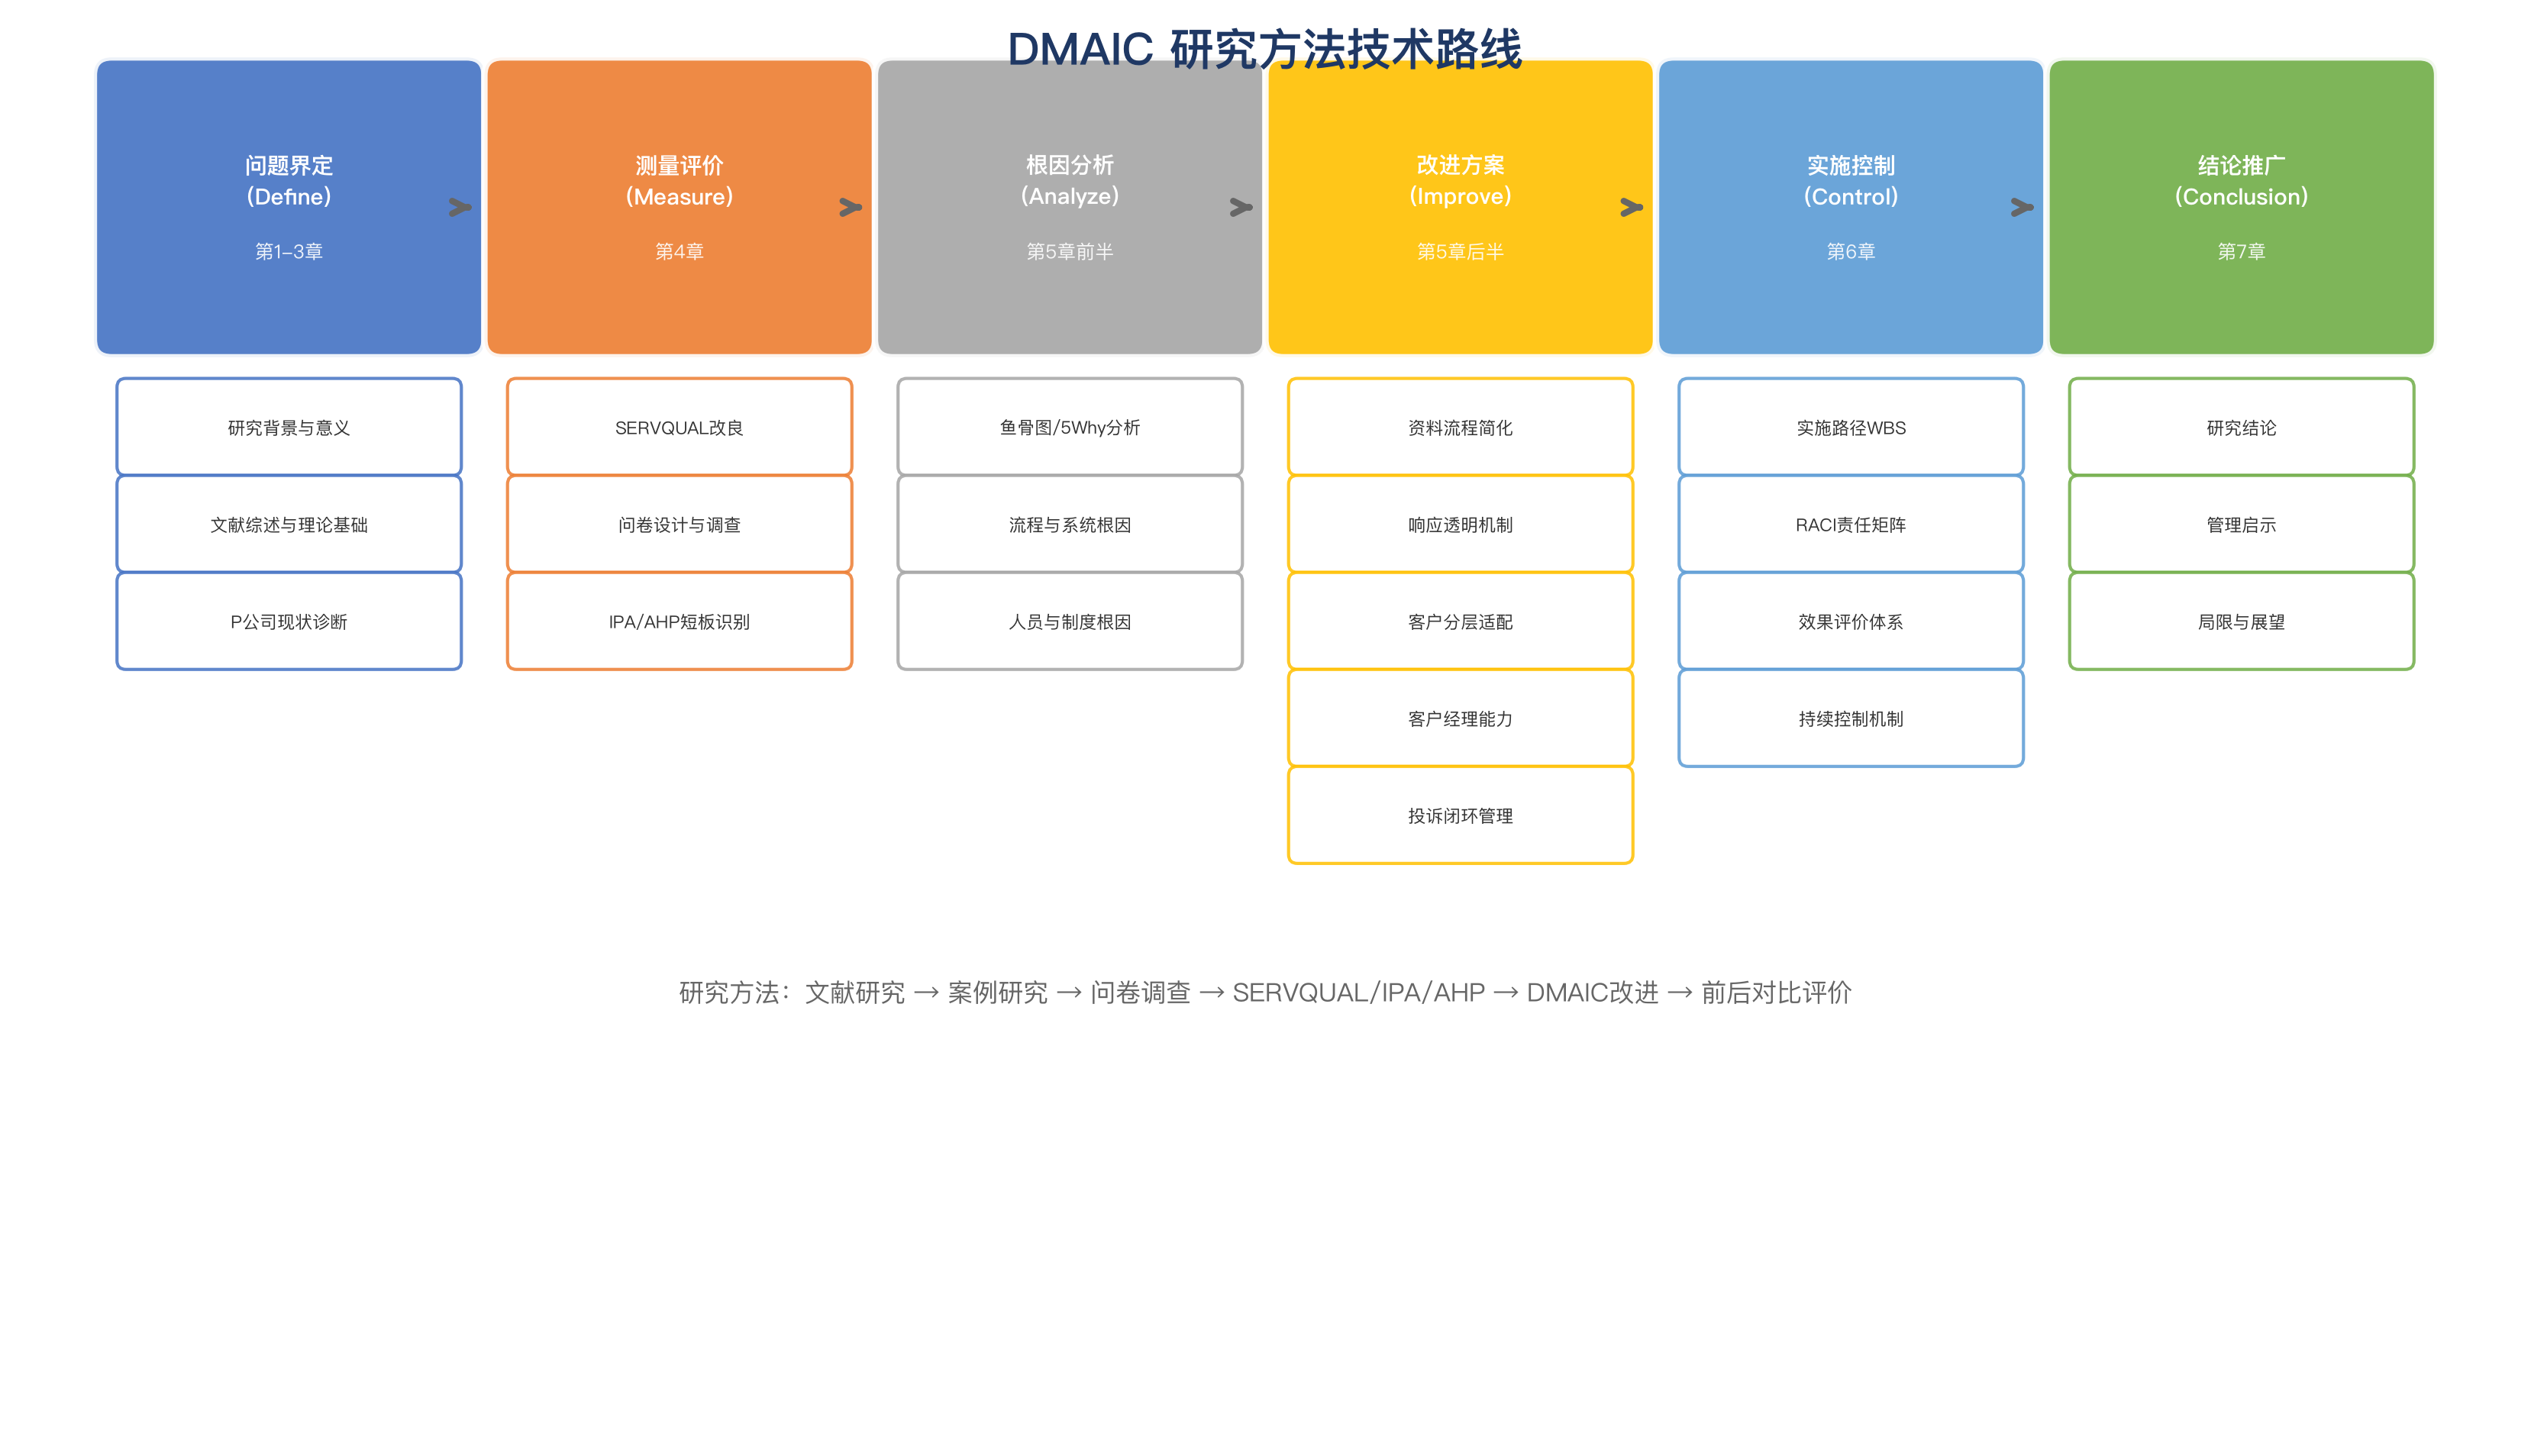
\includegraphics[width=0.85\textwidth]{figures/图1-4_技术路线图.png}
  \caption{本文技术路线图}
  \label{fig:1-4}
\end{figure}

\section{1.5 研究贡献与论文结构}

本研究的主要贡献可归纳为以下四个方面。第一，将服务质量评价研究引入小微贷款这一细分金融服务场景，在经典SERVQUAL五维模型的基础上进行场景化改良，增加了便利性、透明性和产品适配三个维度，形成适用于小微贷款服务特征的八维评价框架，回应了该场景中信息不对称程度高、多角色协同复杂的独特特征，在现有文献中较少被系统探讨。第二，构建了IPA四象限与AHP层次分析的组合赋权方法，以重要性—绩效交叉定位初步识别关键短板维度，以AHP定量权重修正经验判断可能带来的偏差，为小微贷款服务质量的短板识别提供了兼具可视化优势和定量化精度的方法工具。第三，将DMAIC闭环方法论应用于普惠金融服务质量改进领域，使质量评价与改进方案形成有机衔接，避免了传统研究中评价活动与改进活动互相割裂的局限\cite{ref12}。第四，设计了包含组织保障、制度保障和系统保障的三层实施保障体系，以及基于SPC统计过程控制思想的持续监测机制，使服务质量的改进效果具备可长期维持的工程化基础，超越了单一项目式改进的短期局限。\par

本文共分为七章，结构安排如下。第1章（绪论）阐述研究背景、研究问题、研究意义、研究内容与方法、研究贡献、论文结构以及研究局限。第2章（文献综述与理论基础）系统梳理普惠金融与小微贷款、金融科技服务模式、服务质量与客户满意度、SERVQUAL/IPA/AHP方法论以及DMAIC方法的研究现状。第3章（P公司小微贷款服务质量现状诊断）基于业务数据和客户调研，全面扫描并描述P公司服务流程中的质量痛点。第4章（服务质量评价模型的构建与测量）阐述SERVQUAL改良八维模型的设计逻辑与问卷测量结果。第5章（改进方案设计）针对识别出的核心短板及其根因，设计覆盖关键服务环节的工程化改进方案。第6章（实施保障与效果评价）设计组织、制度、系统三层保障体系并对改进方案的效果进行验证与评估。第7章（结论与展望）总结研究发现并提出未来研究方向。服务质量改进作为贯穿P公司小微贷款业务增长与风险控制的核心主线，在全文各章节中层层展开、逐步深化。\par

\section{1.6 研究局限与边界}

本研究存在若干方法论层面的局限，主要包括研究者角色偏差（研究者在P公司担任服务质量改进项目负责人）、样本非回应偏差（有效回收率60.8\%）、单一案例可推广性限制、AHP专家小组规模限制（5位专家处于方法下限）及共同方法偏差风险等。上述局限在第4章4.7节和第7章7.3节中有更充分的讨论。本章在此仅作简要提示，以帮助读者在研究之初了解本文的方法论边界。\par

\chapter{文献综述与理论基础}

本章围绕研究问题，按"业务背景 → 服务模式变化 → 服务质量评价 → 测量方法 → 改进路径 → 研究空白"的概念链条展开文献综述。全章共六节，依次梳理普惠金融与小微贷款、金融科技服务模式、服务质量与客户满意度、SERVQUAL/IPA/AHP评价方法、DMAIC服务流程改进五条研究脉络，最后通过文献述评明确现有研究的不足与本文的定位。\par

\section{2.1 普惠金融与小微贷款研究}

小微企业的融资约束问题在学术界已形成较为系统的认识。其成因可从信息不对称、抵押不足、征信缺失与交易成本偏高四个维度加以理解。其一，小微企业普遍缺乏规范的财务报表和可验证的信用记录，金融机构难以准确评估其还款能力与还款意愿，由此形成严重的事前信息不对称，这种信息不对称还会引发逆向选择：风险较低的企业因无法自证信用而退出市场，留在信贷池中的企业平均风险上升，迫使金融机构进一步提高利率或收紧授信条件。其二，小微企业可用于抵押的固定资产有限，而信用担保体系在覆盖面和运作效率上的不足，使得"抵押缺口"成为制约信贷扩张的刚性约束。其三，小微企业征信信息的碎片化和非标准化特征，导致传统以央行征信报告为核心的授信决策模式面临严重的"信息采集成本-收益不对称"，这种交易成本的结构性偏高进一步压缩了金融机构服务小微的内生动力。上述三方面成因相互叠加，共同构成了小微企业融资难、融资贵的系统性根源。\par

上述信息不对称引发信贷配给的经典理论根源，可追溯至Stiglitz和Weiss（1981）的信贷配给理论\cite{ref17}。该理论证明，在信息不完美条件下，银行提高利率不仅无法出清超额信贷需求，反而会通过逆向选择和道德风险效应恶化贷款组合质量，因此银行宁愿维持低于市场出清水平的利率并实施信贷配给。该理论为理解小微融资困境提供了根本性的经济学解释：信息不对称是信贷配给的内生原因，破解小微融资困境不能仅依靠利率工具或担保工具，还需要从降低信息不对称、改善服务效率的方向寻找工程管理层面的解决方案。这一点构成了本文聚焦服务质量而非仅关注融资可得性的理论依据。\par

在实证层面，王贤彬等（2025）基于小微支行设立的准自然实验，发现普惠小微信贷供给的扩张显著促进了小微企业的市场进入，这一效应在金融服务相对薄弱的地区尤为明显\cite{ref2}。该研究从供给侧验证了信贷可及性对小微主体活力的关键作用，但其研究视角侧重于机构进入与业务扩张，并未深入讨论信贷服务过程中的客户体验维度。\par

在普惠信贷供给机制层面，政策性担保与风险分担工具被广泛讨论。宋卓霖、赵涵（2024）系统考察了政策性担保在小微融资中的作用边界，指出担保机制虽能部分缓解抵押不足问题，但其效果受制于担保机构的风险偏好和银行的协作意愿\cite{ref18}。这意味着单一的供给端政策难以独立破解小微融资困境，需要配套的信息治理和服务机制跟进。从方法论角度看，该研究提供了一个重要的启示：政策工具的实际效果高度依赖于执行层面的制度设计和流程配套，这恰是工程管理视角的切入点。\par

数字普惠金融的兴起为上述困局提供了新的解决思路。祝树金、朱捷尧（2025）的实证研究表明，数字普惠金融通过降低信息搜寻成本、拓展服务半径和加快资金流转，显著促进了中小微企业在价值链中的攀升\cite{ref7}。顾锋娟等（2024）利用省级面板数据进一步揭示，数字普惠金融对小微融资的促进效应存在地区异质性，东部地区的改善幅度大于中西部，这提示数字化红利的释放需要配套的基础设施和制度条件支撑\cite{ref21}。周雷等（2024）的研究则从数字普惠金融服务模式创新角度，探讨了如何通过场景化服务和信用信息共享缓解小微融资堵点\cite{ref22}。\par

国际研究同样提供了有力的对照证据。Yao和Yang（2022）基于中国创业板上市公司数据，发现数字金融通过缓解融资约束间接驱动了中小企业创新，其传导机制主要包括降低融资成本和缩短审批周期\cite{ref6}。Lu等（2021）的实证工作则聚焦于本地银行的作用，发现本地银行与数字金融的协同能够更有效地缓解中小企业的融资约束，这一"线上线下互补"的发现为理解服务渠道融合模式提供了实证基础\cite{ref13}。Zhang等（2023）的研究发现，数字普惠金融通过缓解融资约束促进中小企业技术创新，且这一效应在金融监管较强和政府补贴较充裕的环境下更为显著\cite{ref23}。\par

纵观上述文献，现有研究主要围绕"融资可得性"展开，即关注小微企业能否获得贷款、以什么成本获得贷款。这一视角虽然抓住了小微融资的核心矛盾，但在以下方面存在明显不足：贷款服务过程中的客户体验问题，包括申请便捷度、审批透明度、客户经理专业性和贷后服务质量等，尚未进入主流研究视野。对P公司这样的普惠金融机构而言，客户在申请、审批、放款、贷后各环节中感知到的服务效率、信息透明度和专业支持，同样构成了业务可持续性的关键变量。因此，本文主张将研究焦点从"融资可得性"适度扩展至"融资服务质量"，二者并非替代关系，而是互补关系。\par

\section{2.2 金融科技与小微贷款服务模式}

数字技术的快速渗透正在重塑小微贷款的服务模式。大数据风控使金融机构能够在缺乏传统抵押和财务报表的条件下，通过多维度替代数据（如经营流水、税务记录、线上行为轨迹）构建信用评估模型\cite{ref10}。汪勇等（2026）利用助贷机构数据证实，数字金融技术显著降低了借贷双方的信息不对称程度，但这种改善效果在客户数字素养较低或线上线下流程衔接不畅的场景中有所衰减\cite{ref10}。这一发现揭示了一个核心命题：技术赋能并非自动转化为服务体验提升，二者之间存在需要管理的"转化缺口"。\par

从服务模式演进的视角观察，小微贷款业务正经历从纯线下到线上线下融合、从纯人工到人机协同的转变。韩莉等（2021）在对金融科技助力小微企业融资的文献评析中，系统梳理了智能审批、线上获客、区块链征信等技术在小微信贷中的应用进展，同时指出一个关键缺失：多数研究关注的是技术本身的效率和精度，对技术嵌入后的客户体验变化着墨不多\cite{ref9}。Dumitrescu等（2021）将机器学习方法引入信用评分领域，证实了非线性决策树模型在预测精度上优于传统逻辑回归，但模型的可解释性下降可能带来新的客户信任问题\cite{ref24}。这一发现的管理含义在于：信用评分的技术进步如果以牺牲透明性为代价，可能在提升审批效率的同时损害客户对公平性的感知。\par

服务模式变革的另一面是"体验断点"的出现。线上流程虽然缩短了物理距离，但也可能拉大服务鸿沟。Davis（1989）提出的技术接受模型（TAM）以感知有用性和感知易用性为核心变量，系统解释了用户对信息技术系统的接受行为\cite{ref25}。Nugraha等（2022）针对印度尼西亚中小企业的调查发现，金融科技采纳意愿受到感知易用性和社会影响的显著驱动，但在实际使用中，用户对平台操作复杂、问题响应延迟、缺乏人工支持的抱怨较为普遍\cite{ref26}。相似的问题在中国语境下同样存在：线上申请虽然便捷，但当客户遇到资料补正、审批进度不明、退件原因笼统等情况时，缺乏有效的沟通渠道将加剧焦虑和不信任。吴勇民（2026）从金融大模型赋能供应链融资的视角，讨论了智能技术在融资服务中的双重效应：一方面提升了流程效率，另一方面也产生了新的协调成本和技术门槛\cite{ref27}。\par

对本研究而言，上述文献提供了两重启示。第一，数字技术是改善小微贷款服务质量的工具，不是目的。第二，技术引入与服务质量之间不存在天然的线性关系，需要系统性的服务设计和管理机制来弥合其中的落差。这恰好是DMAIC方法论的价值所在。\par

\section{2.3 服务质量与客户满意度研究}

服务质量（Service Quality）作为一个具有独立理论地位的管理概念，经历了从北欧学派到北美学派的概念化过程。Grönroos（1984）最早提出顾客感知服务质量模型，将服务质量区分为技术质量（what，即服务的结果）和功能质量（how，即服务的过程）。这一区分的价值在于：它指出了服务质量评价的双重维度，客户不仅关心"得到了什么"，也关心"是如何得到的"。Parasuraman、Zeithaml和Berry（1988）在此基础上发展出SERVQUAL量表，以期望-感知差距为核心逻辑，将服务质量操作化为可测量的多维度构念\cite{ref14}。Cronin和Taylor（1992）提出的SERVPERF模型则以绩效直接测量替代差距测量，认为仅测量感知绩效即可有效反映服务质量\cite{ref29}。该理论框架的基石在于一个根本性的认知：服务质量不是由服务提供者定义的，而是由客户通过比较事前期望与事后感知来判定的。这一认知范式对服务管理的颠覆性在于，它将质量定义权从供给侧转移到了需求侧。\par

在服务质量的结果变量方面，学术界积累了较为一致的经验证据。Nguyen等（2020）以银行业为背景，验证了"服务质量 → 客户满意度 → 转换成本 → 客户忠诚度"的完整关系链，其中服务质量对满意度的直接效应最为显著，而满意度在服务质量与忠诚度之间发挥部分中介作用\cite{ref31}。这一发现的管理含义是明确的：服务质量是可管理的前置变量，通过改进服务质量来提升满意度和忠诚度，比直接干预满意度或忠诚度更具操作可行性。在金融服务领域，该链条还获得了定量化的经验支持：服务质量每提升1分（5分制），客户忠诚度平均提升约0.6分，转换成本的提高进一步锁定了客户关系\cite{ref31}。Zaheer（2023）以银行业为对象，运用结构方程模型（SEM）进一步验证了SERVQUAL各维度对客户服务质量的差异化影响，为多维服务质量结构提供了统计证据\cite{ref32}。\par

上述关系链的理论基础可进一步追溯至Heskett等（1994）提出的服务利润链理论\cite{ref33}。该理论阐明了服务企业经营绩效的因果传导逻辑：内部服务质量驱动员工满意度，员工满意度驱动员工保留与生产率，进而创造外部服务价值；客户感知的服务价值驱动客户满意度，客户满意度驱动客户忠诚度，而客户忠诚度最终驱动收入增长和利润提升。在金融服务语境下，服务利润链将服务质量改进从成本中心重新界定为利润驱动要素：服务质量管理的目的不仅在于消除投诉，更在于构建可持续的客户关系和竞争优势，从而为普惠金融机构的服务质量投入提供了商业合理性论证。\par

银行业服务质量研究为本文提供了直接的参照系。Siddiqi（2011）针对孟加拉国零售银行的实证研究表明，服务质量各属性对客户满意度的影响存在显著差异，其中可靠性和响应性的贡献最大，有形性的贡献最小，这一发现与金融服务的无形性特征相符\cite{ref35}。Kheng等（2010）在马来西亚槟城银行的调查中得出了相似结论，并进一步发现服务质量对客户忠诚度的影响主要通过满意度的中介路径实现，这意味着即便服务质量得到改善，如果没有转化为客户可感知的满意度提升，其对忠诚度的拉动作用将大打折扣\cite{ref36}。在国内研究方面，孙彦佩（2025）以ZY银行郑州分行为案例，从网点服务流程的角度系统诊断了服务质量短板，其问题维度分类（人员服务、流程效率、信息沟通、环境设施）对本文第3章的现状诊断具有方法参考价值\cite{ref37}。黄兆锟（2025）聚焦于小微企业客户关系管理的优化，揭示了小微客户在贷款服务中对及时响应和个性化服务的高度敏感性，这种敏感性显著高于零售个人客户\cite{ref38}。\par

数字化转型为服务质量研究带来了新的变量。Zouari和Abdelhedi（2021）以伊斯兰银行为例，发现在数字化背景下，客户满意度的影响因素从传统的物理网点体验转向线上平台的可用性和安全性，这一转变的幅度在年轻客户群体中尤为显著\cite{ref39}。Kaur等（2021）针对印度北部数字银行的研究则提出了一个值得警惕的发现：数字化在提升便利性的同时，也引入了网络安全、数据隐私和服务中断等新型风险感知，这些风险感知对满意度存在显著的负向影响，其效应量在某些场景下甚至超过了便利性提升带来的正面收益\cite{ref40}。上述发现对本文的启示在于：小微贷款服务质量的评价维度不能简单照搬传统银行的量表，需要纳入便利性、透明性和风险安全等数字化时代的新维度。\par

综合本节梳理的文献，服务质量理论经过近四十年的积累，已经形成了"概念界定 → 维度操作化 → 前因后果验证"的成熟研究范式。在金融服务，尤其是小微贷款场景中，该范式的适用性已经得到初步验证，但针对小微贷款特定场景的维度改良和系统评价的工作仍然不足，这构成本文第4章评价模型的切入点。\par

\section{2.4 SERVQUAL、IPA与服务质量评价方法}

SERVQUAL模型是服务质量评价领域最具影响力的理论工具。Parasuraman、Zeithaml和Berry（1988）提出的经典五维模型将服务质量分解为有形性（Tangibles）、可靠性（Reliability）、响应性（Responsiveness）、保证性（Assurance）和移情性（Empathy），并通过期望-感知差距分值（Gap Score）来量化服务质量水平\cite{ref14}。该模型的核心优势在于：它将抽象的服务质量概念转化为可测量、可比较、可追踪的指标体系，为服务改进提供了量化起点。然而，SERVQUAL的通用性也是一把双刃剑，不同行业、不同服务场景需要根据自身特征对维度和指标进行酌情调整，这是模型应用中的基本共识。\par

在小微贷款服务场景中，经典五维的覆盖范围存在三个明显缺口。第一，数字渠道已成为小微贷款获客和受理的主要入口，便利性（如线上操作便捷度、材料一次告知率）直接影响客户的第一感知，但经典五维并未系统纳入。第二，小微贷款涉及复杂的费用结构和审批规则，透明性（如费用事先说明、进度实时可查）是建立客户信任的基础，同样是经典五维的盲区。第三，小微客户在经营周期、行业特征和资金需求上的异质性要求产品具备一定的适配弹性，这是服务针对性而非通用移情性的体现。因此，本文在第4章构建改良SERVQUAL模型时，将在经典五维基础上增加便利性、透明性和产品适配三个新维度，形成八维评价框架。\par

IPA（Importance-Performance Analysis）方法为服务质量改进的优先级排序提供了分析工具。花青青等（2025）基于SERVQUAL-IPA模型对P银行J支行的金融机构服务质量进行了评价，以重要度为横轴、满意度为纵轴构建四象限矩阵，将指标分为"优先改进区""继续保持区""供给过度区"和"低优先区"\cite{ref15}。该方法的逻辑简明而有力：资源永远是有限的，服务质量改进不应追求"补齐所有短板"，而应聚焦于"高重要度-低满意度"象限中的关键指标。这种以数据驱动优先排序的思路，与DMAIC方法论中的Measure和Analyze阶段高度契合。\par

在服务质量评价的赋权方法方面，AHP（层次分析法）为多准则决策提供了结构化的权重确定框架。Moslem等（2023）在对AHP应用的系统综述中确认，该方法适用于服务质量评价中多维度、多指标的权重分配，但特别强调了两个使用边界：第一，判断矩阵必须依赖于领域专家的真实判断，不得由研究者自行填写；第二，一致性检验（CR < 0.1）是权重有效性的必要条件\cite{ref41}。Nguyen等（2022）在港口服务质量研究中将模糊AHP与IPA组合使用，先用AHP确定各维度的客观权重，再用IPA识别改进优先项，该方法组合为本文第4章提供了跨行业的方法参照\cite{ref42}。需要指出的是，港口服务与小微贷款服务在客户群体、服务流程和评价维度上存在本质差异，该方法组合在金融服务中的适用性尚需结合行业特征进行验证和调整。\par

线上服务质量的维度扩展也为本文的模型改良提供了依据。Raza等（2020）提出的改良e-SERVQUAL模型，在原五维基础上增加了网站设计、隐私安全和客户服务等线上特有维度，其研究证实线上渠道的服务质量维度结构与传统线下渠道存在显著差异\cite{ref43}。田越（2023）在邮储银行J支行的客户满意度研究中，运用AHP对服务质量指标进行了分层赋权，其指标体系的构建逻辑（先分层、后赋权、再排序）对本文的问卷设计具有参考价值\cite{ref44}。\par

综合本节讨论，SERVQUAL提供了测量框架，IPA提供了优先级排序工具，AHP提供了权重确定方法，三者构成了一套完整的服务质量评价组合工具箱。该组合工具在零售银行、线上银行和部分服务业中已有应用，但在小微贷款场景中的系统性应用尚属空白，这正是本文第4章的核心贡献点。\par

\section{2.5 DMAIC与服务流程改进研究}

DMAIC是由精益六西格玛方法论衍生出的结构化改进模型，包含Define（界定）、Measure（测量）、Analyze（分析）、Improve（改进）和Control（控制）五个阶段。该模型的核心逻辑是：以数据驱动的方式识别问题、测量差距、分析根因、设计改进方案并建立持续控制机制，最终实现流程绩效的可测量改善和制度化固化。与一般管理建议或经验驱动的改进方式相比，DMAIC强调"以事实和数据说话"，要求每一个改进决策都建立在可验证的证据基础之上。这一特征使得DMAIC天然适合应用于服务质量改进这样的多触点、多维度的复杂问题场景。\par

精益六西格玛在金融服务领域的应用已经积累了可观的实证证据。Vashishth等（2024）在金融服务领域的实证研究表明，精益六西格玛方法通过减少流程变异和消除浪费，能够显著缩短服务周期并提升客户满意度\cite{ref46}。de Koning、Does和Bisgaard（2008）较早论证了精益六西格玛在金融服务中的适用性，指出金融服务的流程化特征和大量可获取的运营数据为DMAIC方法的落地提供了天然条件\cite{ref47}。Guarraia和Schwedel（2008）从行业实践的角度提出，银行在应用精益六西格玛时面临的主要挑战不在于方法本身，而在于如何将项目目标与客户体验指标有效对齐\cite{ref48}。这一观点对本文具有直接的指导意义：服务质量导向的DMAIC改进，必须将客户感知指标（而不仅是内部效率指标）作为Define阶段的核心输出。\par

Adanigbo等（2021）针对金融科技产品客服中心的运营延迟问题，设计了基于精益六西格玛的改进框架，证实了DMAIC在缩短响应时间、降低投诉升级率方面的显著成效\cite{ref49}。Delahoz-Dominguez等（2024）将六西格玛与DEA（数据包络分析）相结合，构建了银行服务质量评估与改进的双阶段框架：第一阶段用DEA识别效率前沿面，第二阶段用六西格玛方法设计改进路径\cite{ref50}。该研究在评估方法上的探索对本论文第6章的效果评价指标体系设计具有借鉴意义。\par

在国内研究方面，若干学位论文为DMAIC在银行服务改进中的应用提供了场景参考。孙启蒙（2023）以农行T支行为对象，运用精益六西格玛方法对零售业务服务质量进行了系统改善，其DMAIC五阶段的实施路径为本文的第5章框架设计提供了参照\cite{ref12}。唐家驰（2025）基于六西格玛理论对N银行Y分行网点服务管理进行了优化研究，在控制阶段提出了看板监控和月度复盘的制度化方案\cite{ref51}。张磊等（2023）从政策扶持与金融科技协同视角，实证检验了小微企业信贷融资的改善路径，为本研究理解普惠金融服务质量改进的政策与技术背景提供了宏观层面的参照\cite{ref52}。黄玉婷（2023）在M公司的客户服务流程优化研究中，将流程改进与人员培训、绩效激励相结合，这种"流程-人员"协同改进的思路对本论文的方案设计具有启发性\cite{ref53}。\par

值得指出的是，上述国内案例虽然提供了DMAIC在金融服务领域应用的实证，但大多聚焦于银行传统业务或内部流程效率，较少触及小微贷款这一细分场景中的服务质量议题。小微贷款服务的特殊性在于：客户群体的异质性高、服务链条长且多触点、数字化与传统人工服务并存、风险控制与服务效率存在张力。这些特征使得DMAIC在该场景中的应用需要更多的场景适配，而非简单的方法套用。\par

\section{2.6 文献述评与研究空白}

基于以上五条研究脉络的系统梳理，本文归纳出以下三个主要研究缺口。\par

缺口一：小微贷款服务质量闭环研究不足。现有普惠金融和小微贷款文献主要关注融资可得性和融资成本，即"能不能贷到"和"以什么价格贷到"\cite{ref2,ref6}。对于小微贷款客户在申请、审批、放款、贷后、续贷等完整旅程中的服务体验，学术界尚未给予充分关注。服务质量文献虽然提供了成熟的评价理论，但其在小微贷款场景中的应用主要集中在银行零售业务，而非普惠金融机构的小微贷款专项业务\cite{ref14,ref15}。二者的交集领域存在明显的研究空白。\par

缺口二：服务质量评价与DMAIC改进在普惠金融场景中脱节。SERVQUAL及其改良模型解决了"如何评价"的问题，IPA和AHP解决了"如何排序"的问题，DMAIC解决了"如何改进"的问题。然而，在现有研究中，这三种工具往往各自为政：服务质量评价论文通常止步于发现差距和提出建议，缺乏从评价到方案设计的工程化转换；DMAIC应用文献则多从内部运营指标出发，较少将客户感知数据作为改进的驱动变量\cite{ref49,ref12}。将"评价 → 排序 → 改进 → 控制"四个环节串联为一个完整闭环的研究，在普惠金融领域尚付阙如。\par

缺口三：持续控制机制薄弱。即便是为数不多的小微信贷服务改进研究，其重点也集中在问题诊断和方案设计阶段，对于改进方案实施后的制度化保障、指标监控、异常预警和效果持续验证着墨甚少\cite{ref50}。DMAIC的Control阶段强调的不是一次性的效果验证，而是建立防止绩效回弹的常态化机制。在小微贷款服务场景中，这种机制设计的缺失意味着改进效果难以持续，同类服务质量问题容易反复出现。\par

基于上述文献缺口，本文的研究定位如下：以P公司小微贷款业务为案例场景，将改良SERVQUAL（八维32指标）评价、IPA/AHP短板识别和DMAIC改进闭环集成在同一框架中，构建"评价测量 → 优先级排序 → 根因分析 → 工程化改进 → 持续控制"的完整工程管理闭环。这一研究定位既继承并整合了前述五条研究脉络的核心成果，又回应了小微贷款服务质量闭环研究的方法论缺失，为该领域提供了一套可操作的集成性分析框架，为同类普惠金融机构的服务质量改进提供了可操作、可复制的方法框架。\par

\subsection*{理论与方法支撑关系图}

章末以文字形式描述本文的理论与方法支撑关系：

\begin{verbatim}
普惠金融/小微贷款背景 ---> 服务质量问题（第2.1-2.2节）
                               |
                     SERVQUAL测量与期望-感知差距诊断（第2.3-2.4节）
                               |
                     IPA/AHP优先级排序与关键短板识别（第2.4节）
                               |
                     DMAIC根因分析与工程化改进方案（第2.5节）
                               |
                     持续控制与效果评价闭环（第2.5-2.6节）
\end{verbatim}

关系图说明：普惠金融文献（第2.1节）解释了"为什么小微贷款服务质量是值得研究的问题"；金融科技文献（第2.2节）说明了"为什么服务模式的变化使服务质量评价和系统改进变得更加紧迫"；服务质量与满意度文献（第2.3节）建立了"客户感知是可以测量和管理的经营变量"这一前提；SERVQUAL/IPA/AHP文献（第2.4节）提供了测量工具和优先级排序方法；DMAIC文献（第2.5节）提供了从测量到改进再到控制的工程化路径。五条研究脉络在本文中不是平行并列的，而是按"背景 → 变量 → 工具 → 路径 → 目标"的逻辑逐层递进，最终在第2.6节汇合于一个集成的MEM闭环框架。P公司内部数据（第3-6章）为该框架提供了案例验证的土壤。\par


\chapter{P公司小微贷款业务服务质量现状与问题诊断}

本章以DMAIC方法论的界定阶段（Define）为主线，系统呈现P公司小微贷款业务的运营全貌、服务流程、服务质量现状数据，并在此基础上识别关键问题，明确后续改进项目的边界与目标。全章数据均来源于P公司内部运营系统、客户投诉记录及初步客户满意度摸底调查。\par

\section{3.1 P公司及小微贷款业务概况}

P公司是一家持牌普惠金融公司，属于非银行金融机构，专注于为小微企业和个体工商户提供经营性贷款服务。近年来，国家持续推进普惠金融政策落地，数字普惠金融的发展也为中小微企业的融资可得性提供了新的支撑\cite{ref7,ref2}。在此背景下，P公司逐步建立了覆盖多省域、多产品线的业务体系。\par

截至分析时点，P公司业务已覆盖5个省份、28个城市，形成了较为稳定的区域服务网络（数据来源：P公司内部运营系统）。公司目前运营3条小微贷款产品线：一是信用贷款产品，授信额度为10万元至100万元，面向经营稳定、征信良好的小微客户；二是担保贷款产品，授信额度为50万元至300万元，适用于能够提供合格担保措施的企业；三是供应链贷款产品，授信额度为30万元至500万元，依托核心企业信用向其上下游小微主体提供融资。三条产品线覆盖了不同资产规模和经营阶段的小微客户需求。\par

在服务渠道方面，P公司形成了线上线下融合的服务体系。线上渠道（App和小程序）承载了约55\%的业务量，客户可以自助完成产品浏览、额度测算和申请提交；客户经理线下服务承接约35\%的业务，通过面对面沟通为客户提供方案咨询和材料指导；另有约10\%的业务经由合作渠道引荐。公司当前活跃贷款客户约3,200户，贷款余额约18亿元。一线客户经理团队约45人，人均管户约70户（数据来源：P公司内部业务系统数据）。从人均管户数量来看，客户经理的工作负荷已处于较高水平，服务质量面临压力。\par

\section{3.2 小微贷款业务服务流程}

P公司小微贷款业务从客户接触到贷款结清，可归纳为七个核心服务环节，各环节的服务质量直接影响客户的整体感知。参考张小敏\cite{ref11}对小微线上贷款流程的优化研究以及李欣春\cite{ref55}对普惠信贷客户触达的分析，本文梳理了P公司完整的服务流程链路，并标注了每个环节存在的服务质量痛点。\par

\begin{table}[htbp]
  \centering
  \small
  \caption{P公司小微贷款业务服务流程与服务质量痛点}
  \resizebox{\textwidth}{!}{%
  \begin{tabular}{p{1.8cm} p{1.2cm} p{1.2cm} p{1.2cm} p{6.6cm}}
    \toprule
    \textbf{环节} & \textbf{标准时效} & \textbf{实际中位数} & \textbf{一次通过率} & \textbf{客户接触点与服务质量痛点} \\
    \midrule
    获客触达 & —— & —— & —— & 线上广告投放、客户经理外呼、存量客户转介；痛点：信息不对称，客户对产品条件和费用结构缺乏事前了解 \\
    申请提交 & 即时 & 即时 & —— & App或小程序自助填写、客户经理线下协助填表；痛点：线上线下存在断点，App端申请后仍需补交纸质材料 \\
    资料审核与补正 & 2工作日 & 4.5工作日 & 62\% & 风控系统初审后，通过短信或电话通知客户补充材料；痛点：补正要求表述笼统（如"材料不齐全"），客户平均补正1.8次，补正率达28\% \\
    授信审批 & 7工作日 & 12工作日 & 72\% & 审批进度仅能被动等待通知，客户无法自主查询；痛点：审批超时严重，进度不透明，客户产生焦虑 \\
    签约放款 & 1工作日 & 2工作日 & 95\% & 电子签约平台完成合同签署，系统自动发起放款并发送到账通知；该环节相对顺畅 \\
    贷后管理 & 按季回访 & 实际半年1次 & —— & 客户经理通过电话或短信进行贷后回访；痛点：回访频率显著低于标准要求，客户经营变化难以及时发现 \\
    投诉处理 & 5工作日闭环 & 7工作日 & 62\%闭环率 & 客户可通过客服热线或线上工单提交投诉；痛点：闭环率偏低，23\%的投诉为重复投诉，缺乏根因回溯机制 \\
    \bottomrule
  \end{tabular}%
  }
\end{table}

从流程数据可以清晰看出，资料审核与补正、授信审批以及投诉处理是三个服务时效偏离标准最为突出的环节。其中，授信审批的实际耗时（12个工作日）接近承诺标准（7个工作日）的两倍，资料补正环节的一次通过率仅为62\%，意味着超过三分之一的申请需要客户反复补充材料，严重影响服务体验。\par

\begin{figure}[htbp]
  \centering
  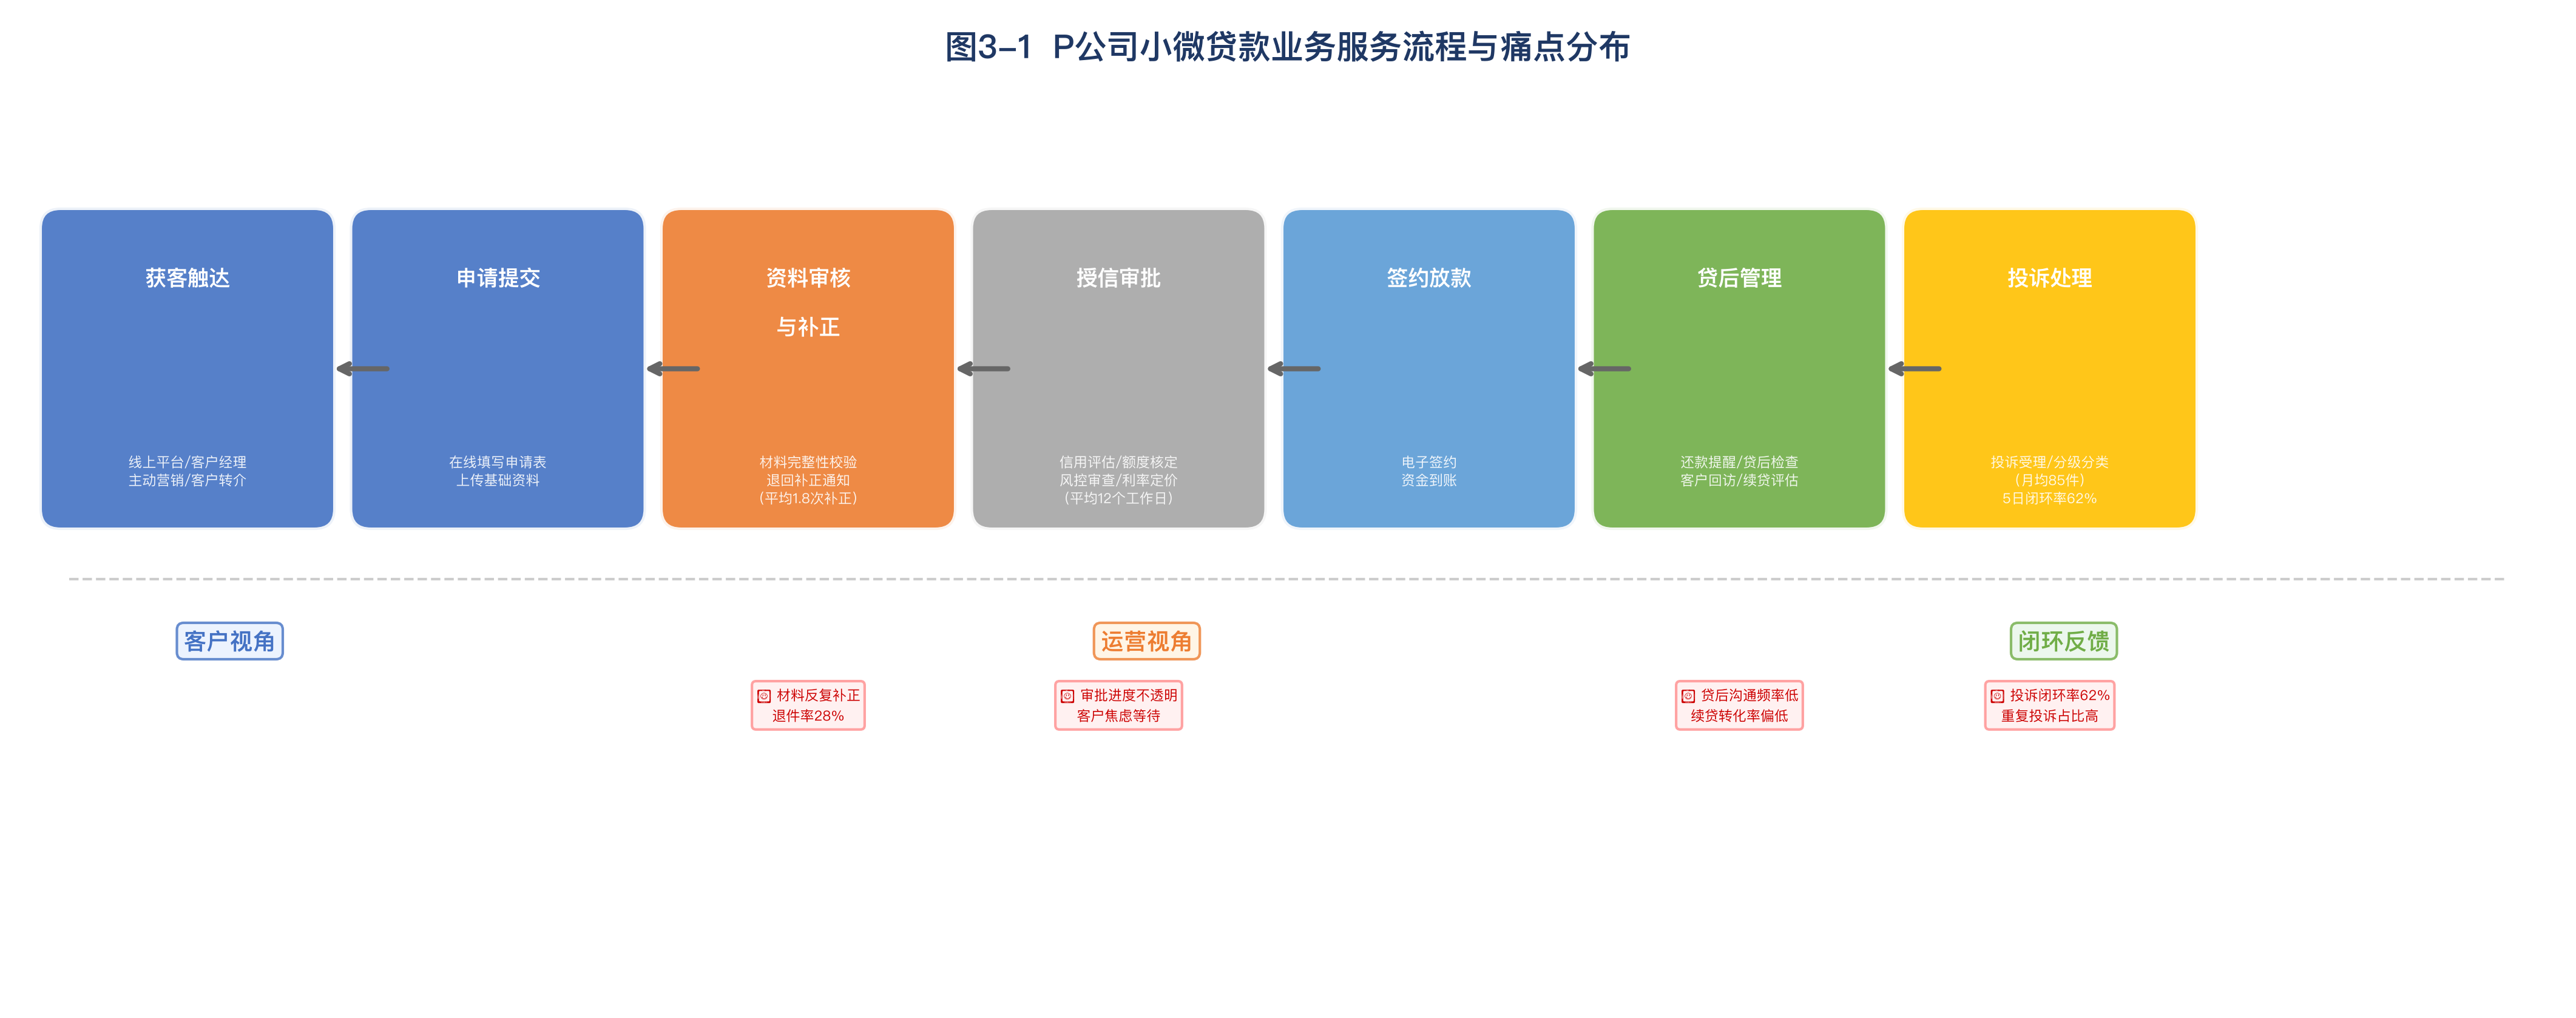
\includegraphics[width=\textwidth]{figures/图3-1_P公司服务流程图.png}
  \caption{P公司小微贷款业务服务流程图}
  \label{fig:3-1}
\end{figure}

\section{3.3 服务质量现状数据}

为进一步量化P公司小微贷款业务的服务质量水平，本节将P公司内部运营数据脱敏后分析如下。参考花青青等\cite{ref15}在金融机构服务质量评价中的指标设计框架，选取了能够反映服务效率、服务准确性和客户反馈的核心指标。\par

\begin{table}[htbp]
  \centering
  \small
  \caption{P公司小微贷款业务服务质量核心指标（近12个月）}
  \resizebox{\textwidth}{!}{%
  \begin{tabular}{p{2.5cm} p{6cm} p{3.5cm}}
    \toprule
    \textbf{指标类别} & \textbf{指标名称} & \textbf{数值} \\
    \midrule
    业务规模 & 业务办理量 & 1,860笔 \\
    服务效率 & 平均办理时长（申请至放款） & 12个工作日（25分位数：5个工作日，75分位数：20个工作日） \\
    服务效率 & 材料补正率 & 28\%（平均每笔补正1.8次） \\
    服务准确性 & 一次通过率（资料无需补正） & 62\% \\
    服务准确性 & 退件率（补正后仍不通过） & 8\% \\
    客户反馈 & 投诉总量 & 1,024件，月均85件 \\
    客户反馈 & 投诉闭环率（5日内解决） & 62\% \\
    客户反馈 & 重复投诉率 & 23\% \\
    客户反馈 & 客户满意度初测（5分制） & 3.12 \\
    \bottomrule
  \end{tabular}%
  }
\end{table}

从数据可以看到，P公司小微贷款业务的服务质量在多个维度存在明显短板。平均办理时长12个工作日表明客户从提交申请到获得放款需要等待近三周，且个案差异极大（75分位数达20个工作日）。材料补正率28\%和一次通过率62\%相互印证，说明近四成客户的申请流程不顺畅。客户满意度初测仅3.12分（5分制），处于"基本满意"与"一般"之间的偏低区间，与行业标杆水平存在显著差距。\par

P公司客诉管理系统记录显示，投诉数据进一步揭示了客户不满的集中方向。对近12个月1,024件投诉的归类分析如下：\par

\begin{table}[htbp]
  \centering
  \small
  \caption{P公司小微贷款业务客户投诉类型分布}
  \resizebox{\textwidth}{!}{%
  \begin{tabular}{p{6cm} p{2cm} p{2cm}}
    \toprule
    \textbf{投诉类型} & \textbf{占比} & \textbf{件数} \\
    \midrule
    审批时效慢 & 32\% & 328 \\
    材料要求不清晰 & 22\% & 225 \\
    客户经理响应慢 & 18\% & 184 \\
    贷款方案不匹配 & 12\% & 123 \\
    贷后服务不足 & 8\% & 82 \\
    费用透明度不足 & 5\% & 51 \\
    其他 & 3\% & 31 \\
    \bottomrule
  \end{tabular}%
  }
\end{table}

审批时效慢和材料要求不清晰两项合计占总投诉量的54\%，是客户不满的首要来源。客户经理响应慢（18\%）和贷款方案不匹配（12\%）分列第三、第四位，反映出服务人员能力和产品设计层面的问题不容忽视。\par

\begin{figure}[htbp]
  \centering
  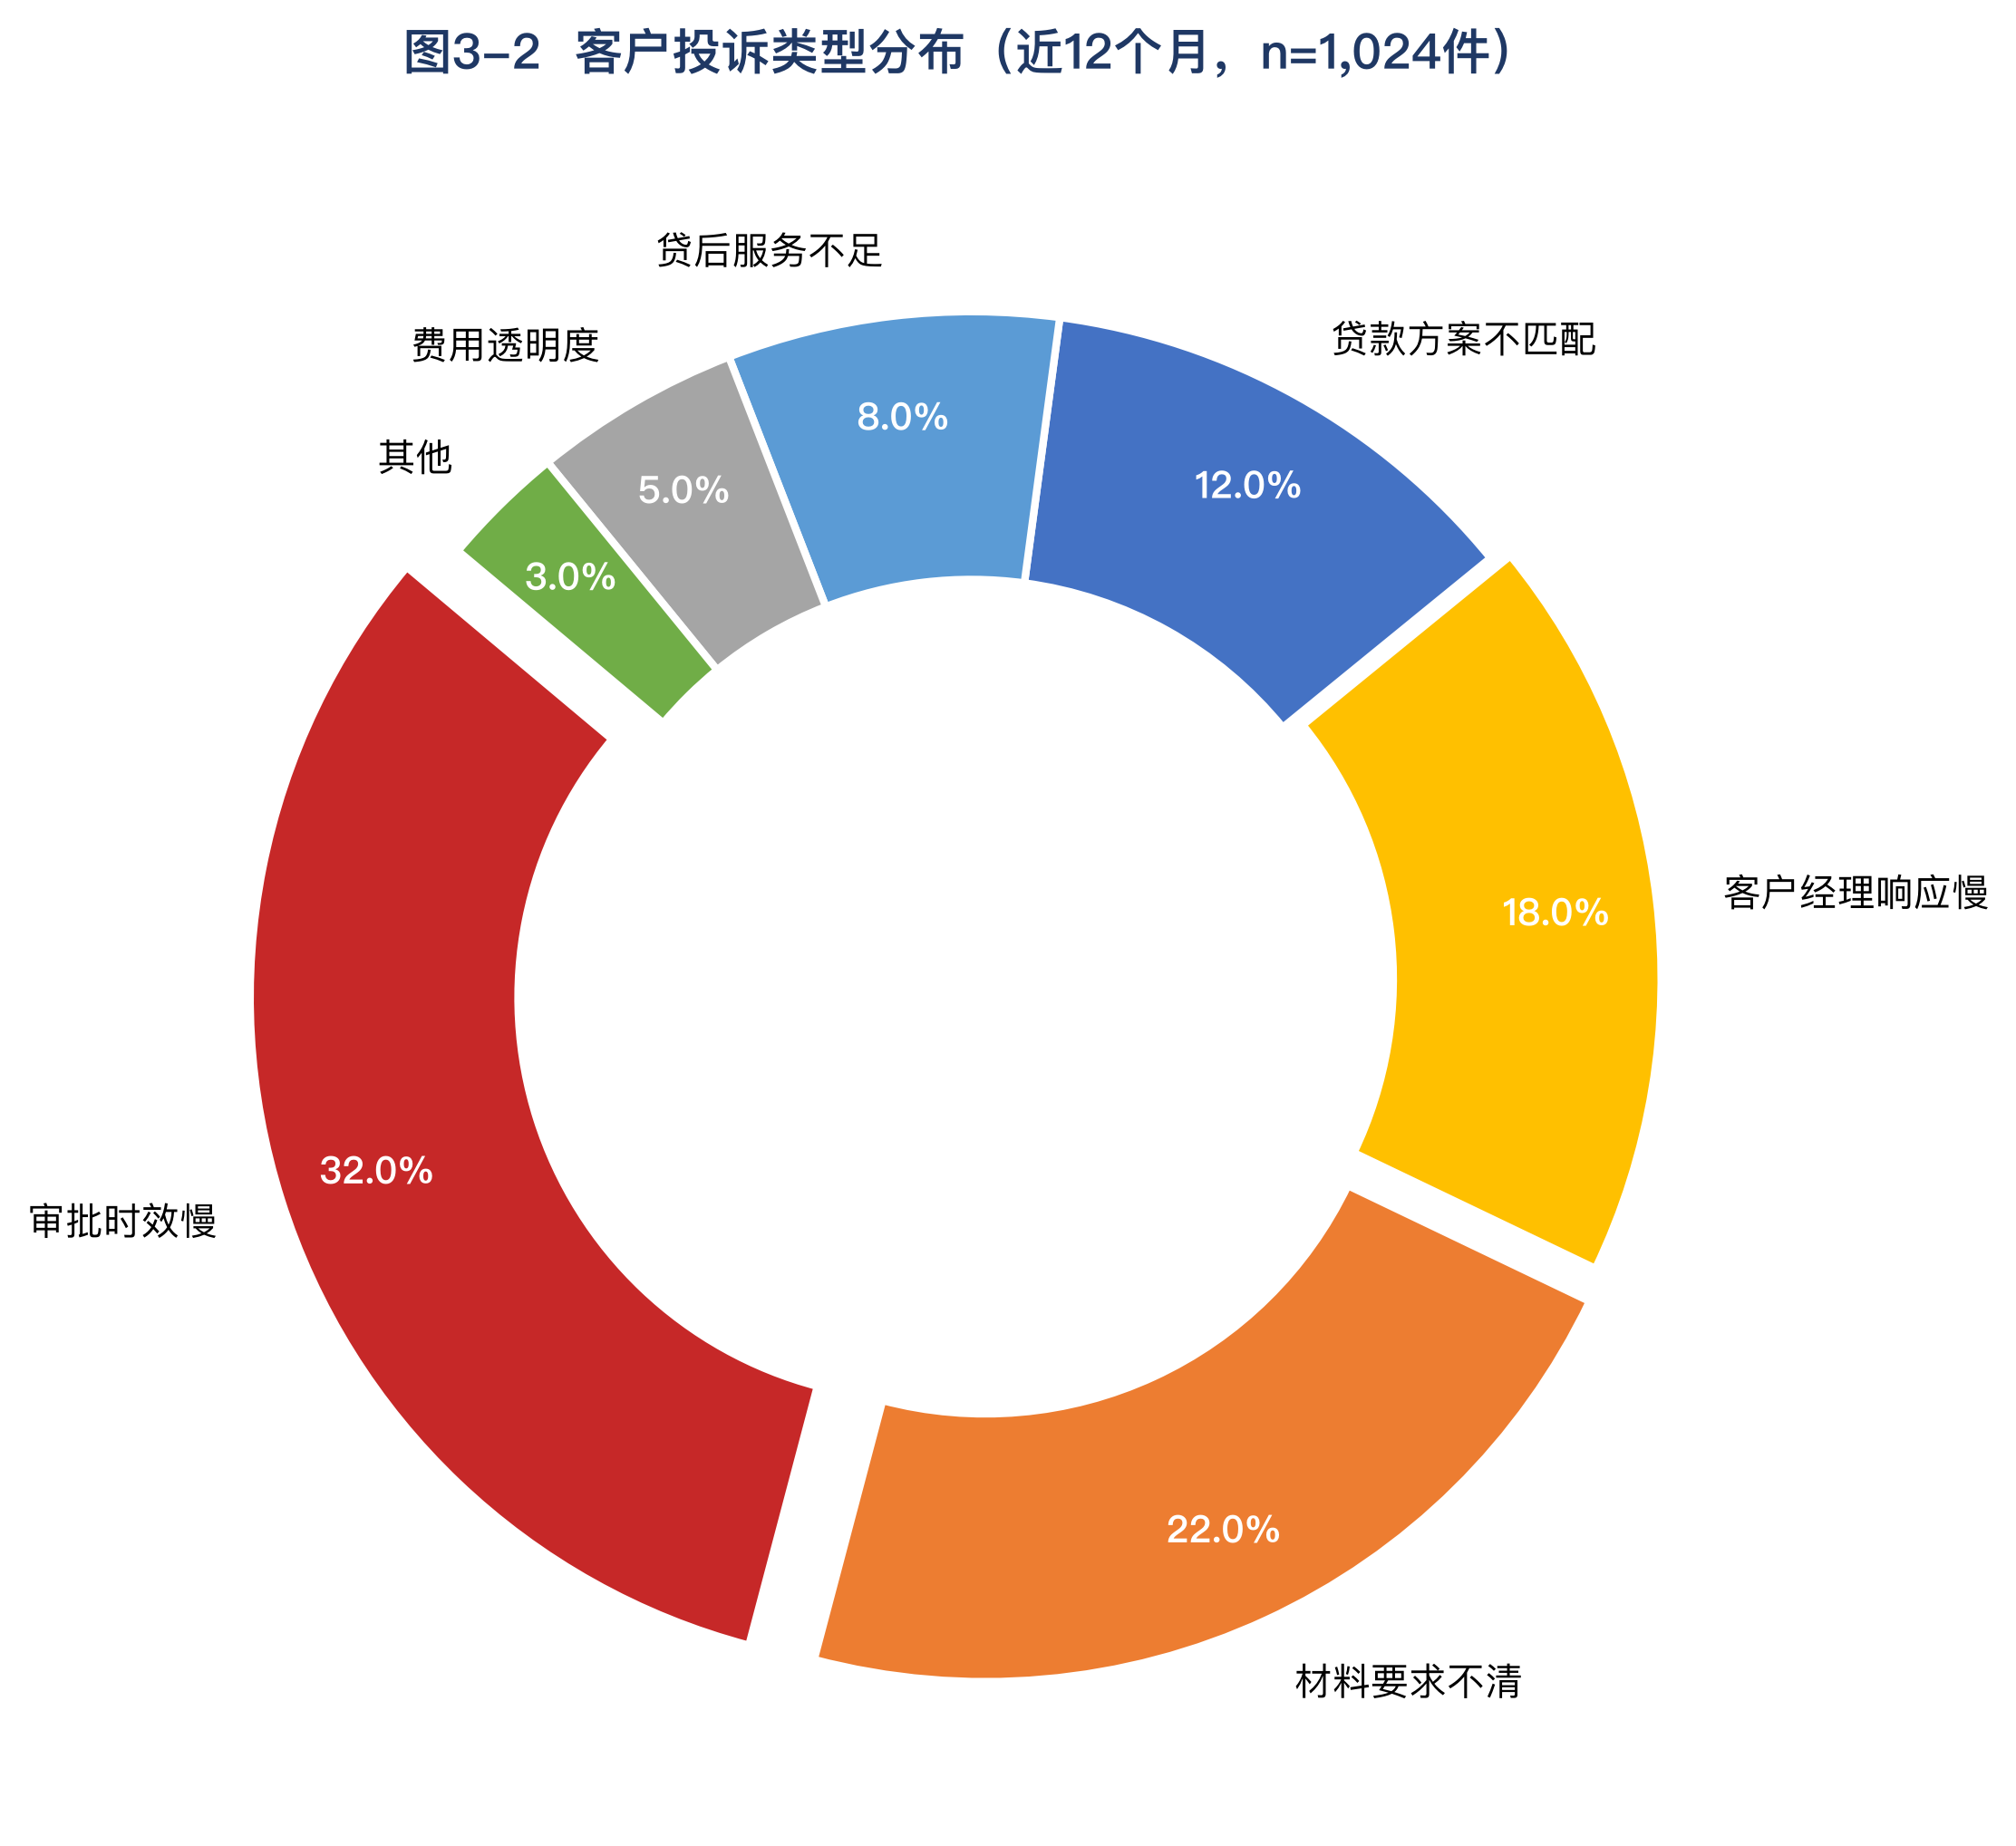
\includegraphics[width=\textwidth]{figures/图3-2_客户投诉类型分布.png}
  \caption{P公司小微贷款业务客户投诉类型分布}
  \label{fig:3-2}
\end{figure}

\section{3.4 主要服务质量问题识别}

基于上述流程分析和现状数据，本节借鉴Parasuraman等提出的SERVQUAL服务质量评价模型\cite{ref14}的维度框架，结合花青青等\cite{ref15}、孙彦佩\cite{ref37}和黄兆锟\cite{ref38}在金融机构服务质量诊断中的研究实践，从客户旅程视角对P公司小微贷款业务的主要服务质量问题进行系统识别。识别标准为：该问题在投诉数据中有明确占比支撑，或在流程数据中表现为显著偏离承诺标准。\par

\begin{table}[htbp]
  \centering
  \small
  \caption{P公司小微贷款业务主要服务质量问题清单}
  \resizebox{\textwidth}{!}{%
  \begin{tabular}{p{2.2cm} p{2.4cm} p{3.7cm} p{3.7cm}}
    \toprule
    \textbf{问题维度} & \textbf{对应SERVQUAL维度} & \textbf{具体表现} & \textbf{影响} \\
    \midrule
    响应速度慢 & 响应性（Responsiveness） & 授信审批平均耗时12个工作日，远超承诺的7个工作日；资料补正通知周期为4.5个工作日，超出标准2.3倍；客户经理回访频率仅为承诺的一半 & 客户等待焦虑加剧，部分客户因时效过长放弃申请或转向其他融资渠道，客户流失风险上升 \\
    信息不透明 & 透明性$\bigstar$（Transparency） & 审批进度不可实时查询，客户只能被动等待；退件原因表述笼统（如"材料不齐全""资质不符"），缺乏具体指向；费用构成未在事前充分说明 & 信息不透明导致客户反复补正（补正率28\%），增加客户时间成本和负面情绪，严重削弱客户对服务过程的信任 \\
    线上线下断点 & 便利性$\bigstar$（Convenience） & 客户通过App提交电子申请后，仍需线下提交纸质证明材料；线上与线下渠道的信息同步不及时，客户需要重复提供相同信息 & 全流程服务体验割裂，背离数字金融背景下客户对"一次办结"的合理期待，便利性感知显著下降 \\
    产品匹配弱 & 产品适配$\bigstar$（Product Fit） & 标准化产品方案难以灵活匹配不同经营规模、不同生命周期小微客户的差异化资金需求；续贷客户不能享受简化流程 & 客户满意度低、续贷意愿不足；12\%的投诉指向方案不匹配，反映出产品设计与客户实际需求之间存在结构性背离 \\
    客户经理能力参差 & 保证性（Assurance） & 新入职客户经理占比约40\%，对公司产品、政策和审批规则的掌握不够系统，不同客户经理对同一问题的答复口径不一致 & 客户感知到的专业性不足，信任度下降；18\%的投诉涉及客户经理响应慢，表明客户经理能力差距已直接转化为服务质量的显性问题 \\
    投诉闭环差 & 可靠性（Reliability） & 投诉闭环率仅62\%，近四成投诉未在承诺的5个工作日内得到有效解决；重复投诉率高达23\%；缺乏系统化的根因回溯与改进机制 & 同类问题反复发生，投诉处理停留在"个案化解"层面，未能从流程和管理层面消除问题根源，客户对服务可靠性的信心持续受损 \\
    \bottomrule
  \end{tabular}%
  }
  {\footnotesize 注：$\bigstar$标记的维度为针对小微贷款服务场景在经典SERVQUAL五维模型基础上扩展的新维度。}
\end{table}

上述六个问题维度覆盖了从客户首次接触到贷后管理的完整服务链条，相互之间存在关联放大效应。审批时效慢加剧了客户对信息透明的需求，而信息不透明又进一步导致客户反复补正材料，拉长了整体办理时长。客户经理能力参差与投诉闭环差之间也存在传导关系：一线服务能力的不足增加了投诉发生的概率，而投诉处理机制的不健全又使这些问题无法被及时发现和纠正。这些问题的深层原因在于P公司缺乏系统化的服务质量评价和管理机制，服务质量的改进仍停留在零散的、被动响应式的层面。\par

\section{3.5 改进项目边界和目标}

基于上述现状诊断，本文明确后续改进研究的工作边界（数据来源：P公司内部资料）。改进范围聚焦于P公司小微贷款业务的服务质量，不扩展至公司全部金融产品线，也不涉及公司战略、组织架构或信息系统的整体重构\cite{ref10}。\par

改进项目围绕六个核心维度设定目标：一是缩短办理时长，将平均申请至放款周期压缩至承诺标准以内；二是提升材料一次通过率，减少客户反复补正的摩擦成本；三是增强信息透明度，实现审批进度可查询、退件原因可追溯；四是提高投诉闭环率，建立从投诉受理到根因改进的闭环管理机制；五是提升客户满意度，通过服务质量的系统性改进推动满意度评分向行业优秀水平靠拢；六是巩固风险合规底线，确保服务提速不以牺牲风控质量为代价\cite{ref24}。\par

在风险控制方面，依照P公司内部制度文件规定，改进项目明确将不良贷款率控制在2.0\%以内作为硬性约束。服务质量改进的任何措施均需在满足该风控边界的前提下实施，不得以放松授信标准、简化风控流程或降低审批质量来换取服务时效的缩短\cite{ref24}。这一边界条件的设定确保了服务质量改进与风险管理的平衡，也是DMAIC方法中界定阶段确定项目约束的关键步骤。\par

综上所述，第3章通过P公司小微贷款业务的全景刻画、服务流程的系统梳理、服务质量现状数据的定量呈现以及主要问题的维度化识别，完成了DMAIC界定阶段的全部工作。上述诊断结果为第4章构建服务质量评价模型提供了明确的问题导向和实证基础。\par

\chapter{第4章 P公司小微贷款服务质量评价模型构建与测量}

本章承担DMAIC方法论中"测量"（Measure）阶段的核心任务：在前三章完成问题界定和服务现状诊断的基础上，构建适用于小微信贷服务场景的质量评价模型，通过问卷调查获取客户期望与感知的双向数据，以量化方式定位P公司小微贷款服务质量的核心短板，为第5章的根因分析和改进方案设计提供定量依据。\par

\section{评价模型选择依据}

服务质量评价领域存在多种成熟的测量工具，不同模型的服务场景适配性和诊断能力各有侧重。在正式构建评价体系之前，有必要对主流模型进行系统比较，以确定最适合P公司小微贷款服务质量评价的方法论基础。\par

客户满意度指数（Customer Satisfaction Index，CSI）是应用最广泛的宏观满意度测量工具，通过结构方程模型将客户期望、感知质量、感知价值和客户抱怨等潜变量纳入统一框架。然而，CSI侧重于"总体满意度"这一汇总性结果变量，无法揭示服务过程中各触点的具体差距，对服务短板的诊断能力有限。净推荐值（Net Promoter Score，NPS）以"您向他人推荐本服务的可能性"为单一核心问题，简单直观、便于跨组织对标，但同样只能反映客户忠诚度的整体倾向，无法提供可操作的服务改进指向。\par

相较而言，Parasuraman、Zeithaml和Berry于1988年提出的SERVQUAL模型以"期望-感知差距"为理论内核，将服务质量分解为有形性、可靠性、响应性、保证性和移情性五个维度，通过分别测量客户在接受服务前的期望值（Expectation）和接受服务后的实际感知值（Perception），以差距值（Gap = P - E）作为服务质量的操作化指标\cite{ref21}。该模型的核心理念是：服务质量的高低取决于客户感知与服务期望之间的落差大小，而非单一维度的满意度评分。因此，SERVQUAL天然适合用于诊断服务的具体短板，其诊断逻辑——"哪一维度差距最大，哪一维度就是优先改进对象"——与本文DMAIC方法论中"测量驱动分析、分析驱动改进"的闭环逻辑高度契合。Nguyen等的实证研究进一步表明，服务质量通过客户满意度的中介效应显著影响客户忠诚度，这为以服务质量作为P公司小微贷款业务增长抓手的理论链路提供了支撑\cite{ref26}。\par

在选择SERVQUAL作为基础模型的同时，需要明确其与后续分析工具的组合关系。首先，SERVQUAL提供的是"差距在哪"的诊断信息，而IPA四象限矩阵在此基础上补充了"优先解决什么"的决策框架——将各维度的差距值与客户赋予的重要度权重进行交叉定位，区分出"差距大且重要度高"的优先改进项和"差距大但重要度低"的延迟处理项，从而避免资源投入的均匀分布。其次，AHP层次分析法通过专家两两比较将主观经验判断转化为可供比较的定量权重，解决了IPA中重要度仅依赖客户主观期望这一单一来源的局限性，使优先级的排序更具多视角的稳健性。这一"SERVQUAL测量差距 → IPA交叉定位 → AHP组合赋权"的三层分析链路，构成了本文从测量到识别的完整方法论框架，也与MEM论文强调的工程化管理思维——以定量数据驱动资源分配和决策优化——一以贯之。\par

在银行业和金融服务场景中，SERVQUAL模型已得到广泛应用和验证。花青青等基于SERVQUAL-IPA组合方法对金融机构服务质量进行了系统评价，证实了该模型在金融场景中的信度和效度\cite{ref6}。综合比较三类候选模型的诊断能力、场景适配性和与DMAIC方法论的衔接性，本文选择SERVQUAL作为P公司小微贷款服务质量评价的基础模型，并根据小微信贷服务的特殊性进行必要的维度改良。\par

\section{小微贷款服务质量指标体系构建}

\subsection{维度改良的逻辑}

经典SERVQUAL五维模型（有形性、可靠性、响应性、保证性、移情性）诞生于传统面对面服务场景，而P公司的小微贷款业务具有三个显著差异：其一，服务链路长且环节多，从申请到贷后管理涉及线上平台操作、线下客户经理沟通、后台风控审批等多个界面；其二，信息不对称程度高，客户对费用结构、审批规则、退件原因等敏感信息的透明性有强烈需求；其三，小微客户的异质性大，标准化的贷款产品难以匹配不同生命周期、不同行业客户的差异化资金需求。\par

基于上述场景特殊性，本文在经典SERVQUAL五维基础上新增三个维度：便利性（Convenience），衡量客户在申请、签约、查询等环节的全流程线上化体验和渠道可触达性；透明性（Transparency），衡量客户对费用结构、审批进度和退件原因的知情程度；产品适配（Product Fit），衡量贷款方案与客户经营特征的匹配程度。新增维度参照了Raza等关于线上服务质量维度扩展的研究\cite{ref29}、Zouari等关于数字银行满意度的维度探讨\cite{ref24}以及Kaur等关于数字银行体验与风险的实证分析\cite{ref25}，同时融合了田越\cite{ref11}和孙彦佩\cite{ref12}在国内银行服务质量评价中的指标设计经验，以及P公司内部客户访谈反馈和监管合规要求。\par

最终形成的改良SERVQUAL评价指标体系包含8个维度、32个测量指标，模型框架如图4-2所示。\par

\begin{figure}[htbp]
  \centering
  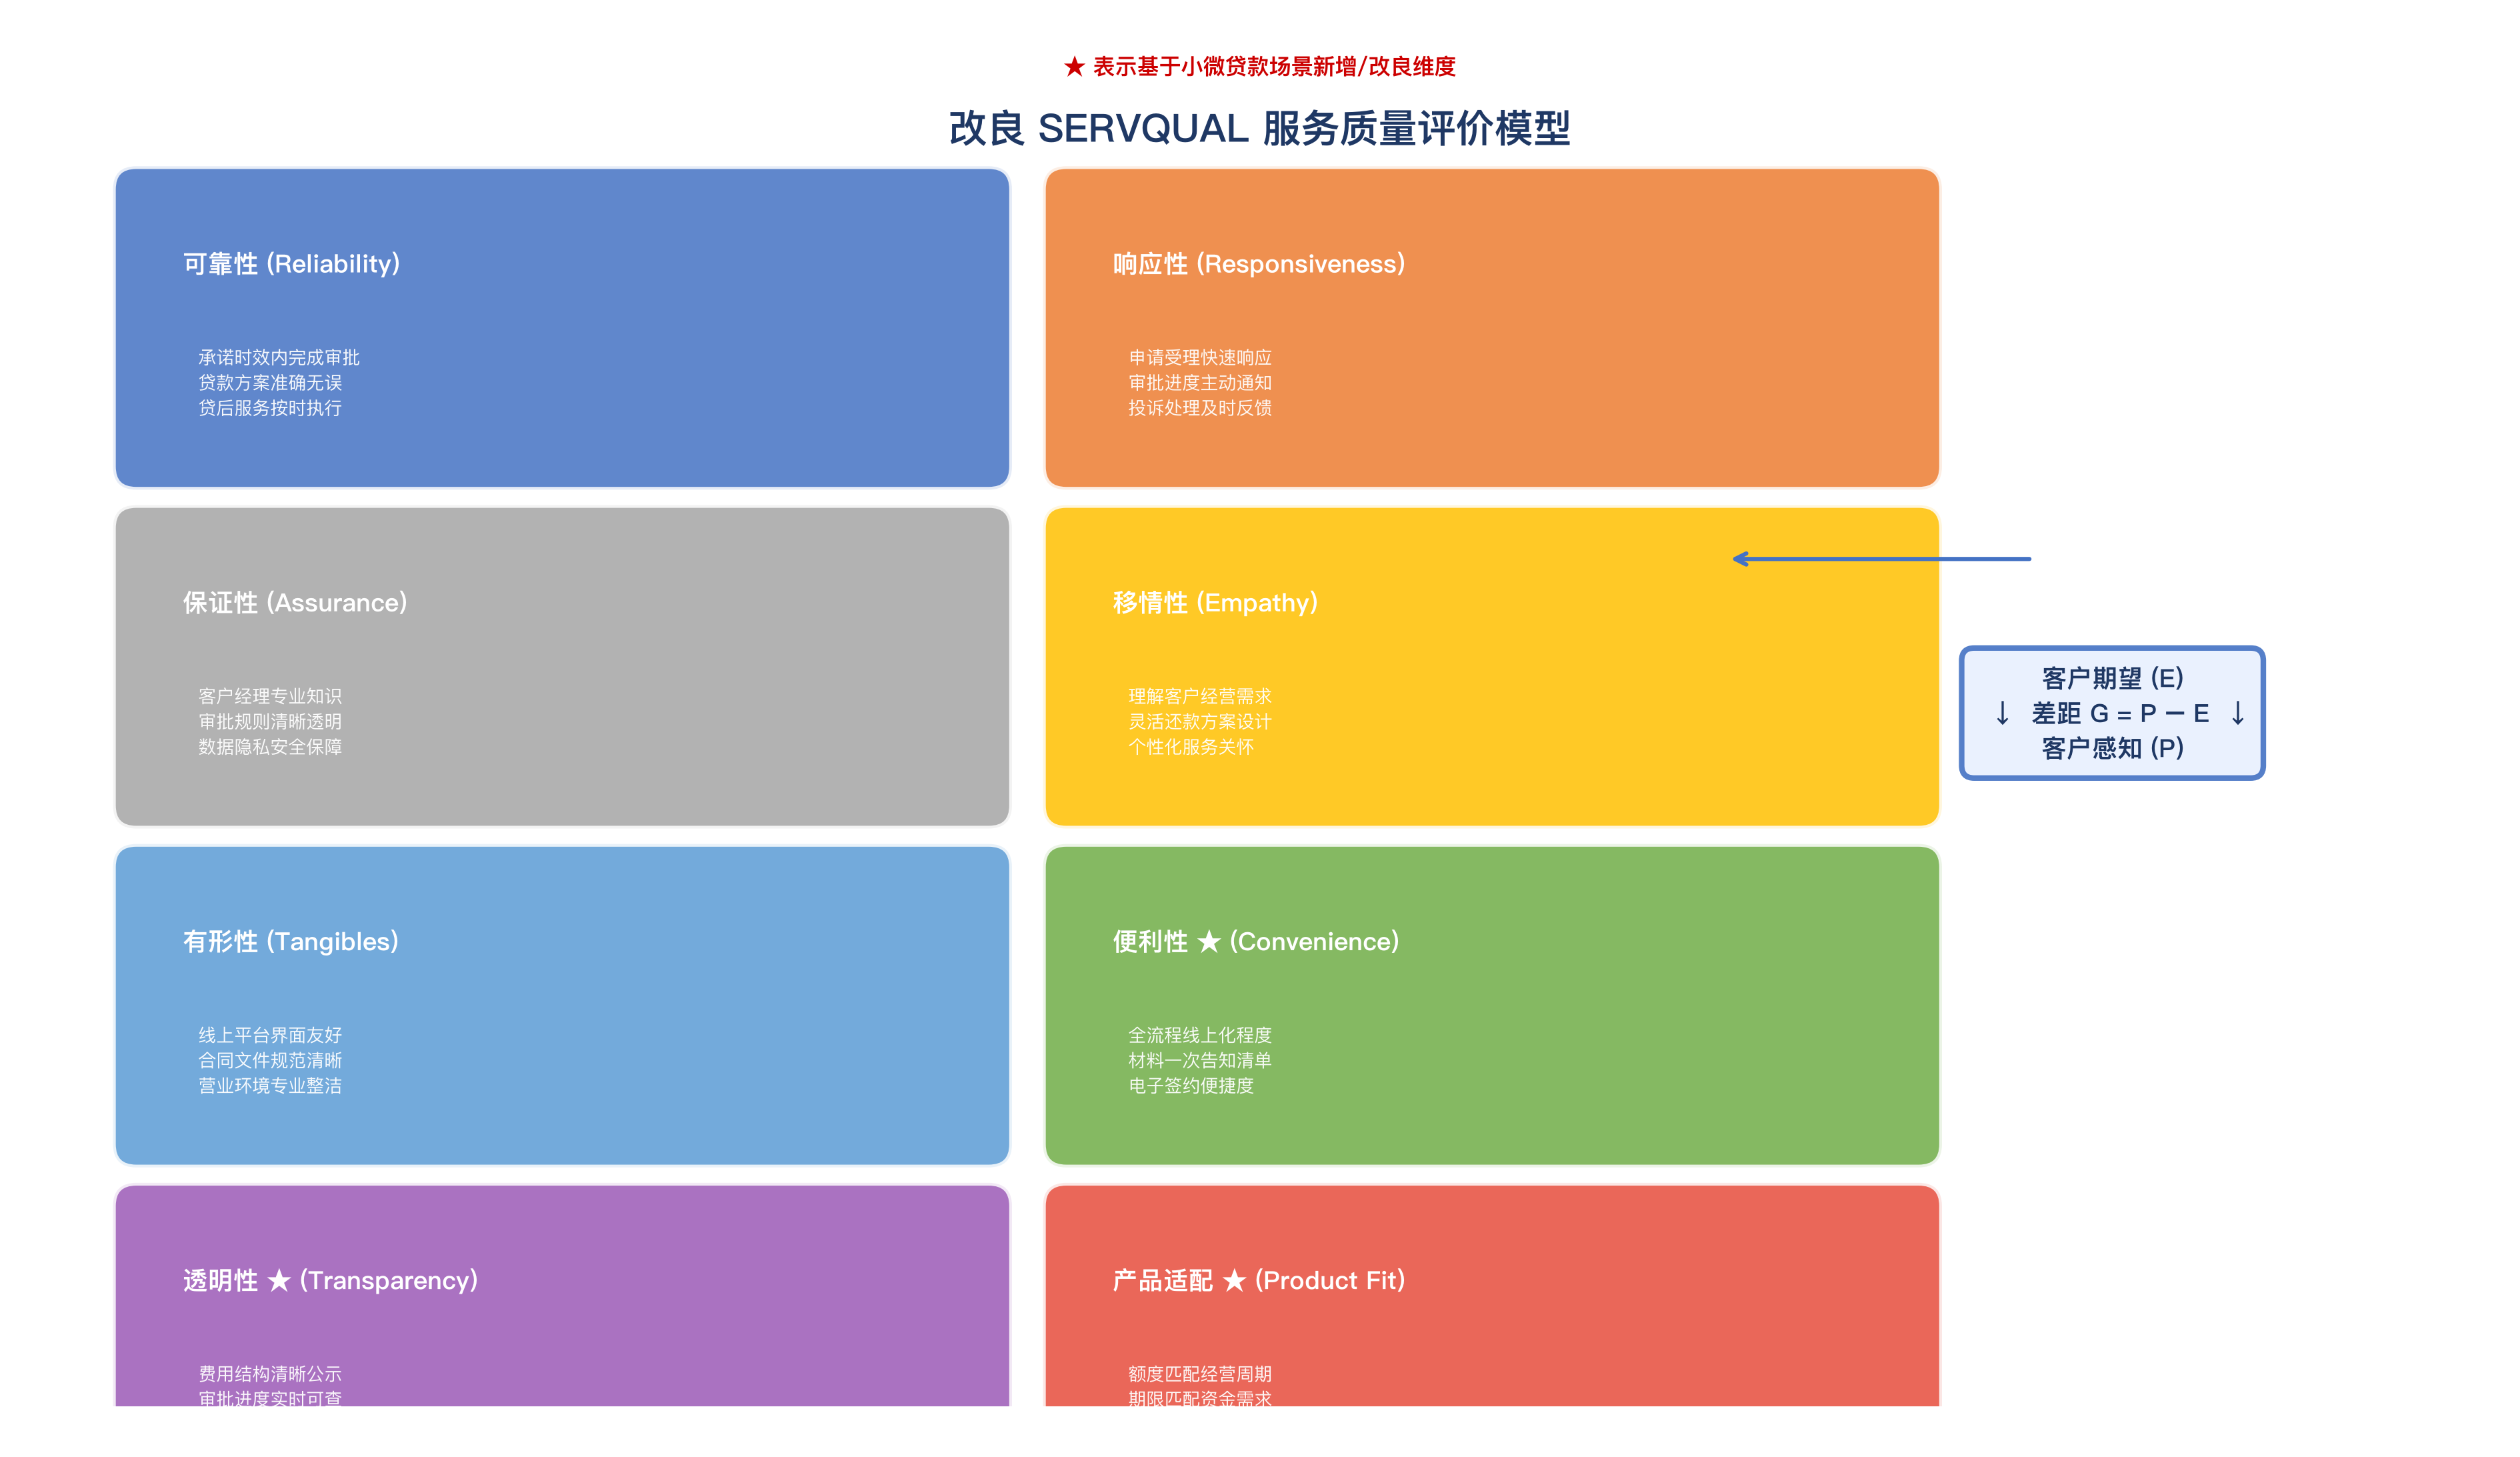
\includegraphics[width=0.85\textwidth]{figures/图4-2_SERVQUAL改良评价指标模型.png}
  \caption{改良SERVQUAL服务质量评价指标模型}
  \label{fig:4-2}
\end{figure}

\subsection{八维32项指标体系}

以下按维度逐一列示指标编号、测量内容和量表来源。各指标均采用李克特五级量表（1=非常不满意/非常不期望，5=非常满意/非常期望），客户分别报告期望值和感知值。\par

（一）可靠性维度（4项）

可靠性衡量服务提供者准确、可靠地履行服务承诺的能力，是小微信贷服务的基础性维度。\par

\begin{table}[htbp]
  \centering
  \small
  \caption{可靠性维度指标体系}
  \begin{tabularx}{\textwidth}{l l l}
    \toprule
    \textbf{编号} & \textbf{指标} & \textbf{量表来源} \\
    \midrule
    SQ01 & 承诺时效内完成贷款审批 & SERVQUAL经典 + 小微场景 \\
    SQ02 & 贷款方案准确无误（额度、利率、期限等） & SERVQUAL经典 \\
    SQ03 & 贷后服务（回访、提醒、结清等）按时执行 & SERVQUAL经典 + 客户反馈 \\
    SQ04 & 投诉处理有明确结论和解决方案 & 客户反馈 \\
    \bottomrule
  \end{tabularx}
\end{table}

（二）响应性维度（4项）

响应性衡量服务提供者主动、及时响应客户需求的能力，直接影响客户的时间成本和焦虑程度。\par

\begin{table}[htbp]
  \centering
  \small
  \caption{响应性维度指标体系}
  \begin{tabularx}{\textwidth}{l l l}
    \toprule
    \textbf{编号} & \textbf{指标} & \textbf{量表来源} \\
    \midrule
    SQ05 & 贷款申请受理后24小时内给予首次响应 & SERVQUAL经典 \\
    SQ06 & 审批进度发生变化时主动通知客户 & 客户反馈 \\
    SQ07 & 拨打客户经理电话3次内能够接通 & 客户反馈 \\
    SQ08 & 投诉受理后24小时内联系客户确认情况 & 客户反馈 \\
    \bottomrule
  \end{tabularx}
\end{table}

（三）保证性维度（4项）

保证性衡量服务人员的专业知识、服务态度及客户对服务安全性的信任程度。\par

\begin{table}[htbp]
  \centering
  \small
  \caption{保证性维度指标体系}
  \begin{tabularx}{\textwidth}{l l l}
    \toprule
    \textbf{编号} & \textbf{指标} & \textbf{量表来源} \\
    \midrule
    SQ09 & 客户经理具备充分的贷款产品知识和风控常识 & SERVQUAL经典 \\
    SQ10 & 贷款审批标准和规则清晰且可理解 & SERVQUAL经典 + 客户反馈 \\
    SQ11 & 客户个人和经营数据的安全有充分保障 & 新增（监管要求） \\
    SQ12 & 客户经理服务态度专业、耐心且友善 & SERVQUAL经典 \\
    \bottomrule
  \end{tabularx}
\end{table}

（四）移情性维度（4项）

移情性衡量服务提供者对客户个性化需求的理解和关怀程度。\par

\begin{table}[htbp]
  \centering
  \small
  \caption{移情性维度指标体系}
  \begin{tabularx}{\textwidth}{l l l}
    \toprule
    \textbf{编号} & \textbf{指标} & \textbf{量表来源} \\
    \midrule
    SQ13 & 客户经理了解客户的经营情况和真实资金需求 & SERVQUAL经典 + 小微场景 \\
    SQ14 & 还款方案（还款日、还款方式等）可根据客户经营周期灵活协商 & 客户反馈 \\
    SQ15 & 贷后主动关心客户的经营状况变化 & SERVQUAL经典 \\
    SQ16 & 在特殊时期（如疫情、自然灾害等）主动提供帮扶方案 & 小微场景新增 \\
    \bottomrule
  \end{tabularx}
\end{table}

（五）便利性维度（★新增，4项）

便利性衡量客户在贷款全流程中的操作便捷度和渠道可触达性，是数字金融服务质量的关键维度。\par

\begin{table}[htbp]
  \centering
  \small
  \caption{便利性维度指标体系}
  \begin{tabularx}{\textwidth}{l l l}
    \toprule
    \textbf{编号} & \textbf{指标} & \textbf{量表来源} \\
    \midrule
    SQ17 & 贷款申请到放款全流程可通过线上完成 & 新增（数字金融趋势） \\
    SQ18 & 申请材料一次性告知且清单明确，无需反复补充 & 客户反馈 \\
    SQ19 & 电子签约流程方便快捷，无需线下往返 & 新增 \\
    SQ20 & 客服可通过多种渠道（App、微信、电话）触达 & 新增 \\
    \bottomrule
  \end{tabularx}
\end{table}

（六）透明性维度（★新增，4项）

透明性衡量客户对贷款服务核心信息的知情程度，是小微信贷服务中信息不对称治理的关键体现。\par

\begin{table}[htbp]
  \centering
  \small
  \caption{透明性维度指标体系}
  \begin{tabularx}{\textwidth}{l l l}
    \toprule
    \textbf{编号} & \textbf{指标} & \textbf{量表来源} \\
    \midrule
    SQ21 & 贷款利率、服务费等费用结构在申请前已清晰说明 & 新增（监管要求） \\
    SQ22 & 贷款审批进度可在线上实时查询 & 客户反馈 \\
    SQ23 & 贷款申请被退回时，退件原因具体、明确 & 客户反馈 \\
    SQ24 & 贷款合同条款表述清晰、易于理解 & 新增 \\
    \bottomrule
  \end{tabularx}
\end{table}

（七）产品适配维度（★新增，4项）

产品适配衡量贷款方案与小微客户经营特征的匹配程度，是提升续贷率和客户黏性的核心维度。\par

\begin{table}[htbp]
  \centering
  \small
  \caption{产品适配维度指标体系}
  \begin{tabularx}{\textwidth}{l l l}
    \toprule
    \textbf{编号} & \textbf{指标} & \textbf{量表来源} \\
    \midrule
    SQ25 & 贷款额度与客户经营规模和资金需求相匹配 & 新增（小微场景） \\
    SQ26 & 贷款期限与客户资金周转周期相匹配 & 新增 \\
    SQ27 & 还款方式灵活可选（等额本息、先息后本等） & 新增 \\
    SQ28 & 贷款到期后的续贷流程便捷高效 & 新增 \\
    \bottomrule
  \end{tabularx}
\end{table}

（八）有形性维度（4项）

有形性衡量服务环境、设备和文件等物理/虚拟载体的专业程度。\par

\begin{table}[htbp]
  \centering
  \small
  \caption{有形性维度指标体系}
  \begin{tabularx}{\textwidth}{l l l}
    \toprule
    \textbf{编号} & \textbf{指标} & \textbf{量表来源} \\
    \midrule
    SQ29 & 线上平台（App/小程序）界面友好、操作流畅 & SERVQUAL经典 + 数字场景 \\
    SQ30 & 贷款合同和申请文件格式规范、清晰 & SERVQUAL经典 \\
    SQ31 & 客户经理着装专业、形象得体 & SERVQUAL经典 \\
    SQ32 & 营业场所环境整洁、设施完善 & SERVQUAL经典 \\
    \bottomrule
  \end{tabularx}
\end{table}

上述八维32项指标体系在保留经典SERVQUAL五维结构效度的基础上，通过新增维度覆盖了小微贷款服务的数字化、透明化、适配性三大场景特征，为后续的问卷测量和统计分析奠定了结构性基础。\par

\section{问卷设计与样本说明}

\subsection{问卷结构}

基于上述指标体系，本研究设计了《P公司小微贷款业务服务质量调查问卷》。问卷由三个部分构成：第一部分为客户基本信息，包含8个题项，涵盖客户的企业类型（个体工商户/小微企业主）、行业类别、经营年限、贷款产品类型、服务渠道偏好和近12个月贷款次数，用于样本特征描述和分组分析；第二部分为服务质量评价核心量表，包含期望量表和感知量表各32个题项（合计64个测量题项），所有题项采用李克特五级评分（1=非常不满意/非常不期望，5=非常满意/非常期望），期望量表要求客户评价"在该项服务上您认为一家普惠金融机构理应采取的标准水平"，感知量表要求客户评价"在最近一次与P公司的业务往来中您的实际感受水平"；第三部分为开放性建议，邀请客户以自由文本形式表达对P公司服务的整体评价和改进建议。\par

问卷设计的结构框式和量表措辞参照了田越在银行对公业务满意度研究中的AHP问卷设计经验\cite{ref11}和孙彦佩关于银行网点服务质量调查的量表构造方法\cite{ref12}，同时结合黄兆锟关于银行小微客户关系管理研究中客户分层的抽样策略\cite{ref18}对客户基本信息部分进行了适配性调整。\par

\subsection{样本与数据采集}

调查对象为P公司近12个月内办理过小微贷款业务的活跃客户群体。调查采用线上线下混合方式进行：线上通过P公司官方App和微信公众号向目标客户推送问卷链接，线下由客户经理在贷后回访和业务办理过程中辅助客户填写纸质或电子版问卷。调查周期为2025年10月至11月，共发放问卷800份，回收问卷510份，经数据清洗（剔除填写时长不足3分钟、量表题项全部勾选同一分值、基本信息严重缺失的无效问卷）后获得有效问卷486份，有效回收率为60.8\%。\par

486份有效样本满足两项因子分析的样本量最低要求：总体样本量N=486大于300，且样本量N与测量题项数p的比值N/p=486/32≈15.2，远高于N/p≥5的建议标准，为后续探索性因子分析和结构效度检验提供了充分的统计效力。\par

\subsection{研究伦理}

本研究严格遵守研究伦理原则。问卷在首页设置了知情同意说明，明确告知客户调查数据仅用于学术研究目的、严格保密且全程匿名处理，客户有权随时退出调查而不影响其与P公司的任何业务关系。所有数据在分析和报告阶段均已脱敏，不包含客户身份信息、企业名称、具体地址和账号数据。P公司已出具研究数据使用授权。\par

\section{信度效度与描述统计}

\subsection{信度分析}

信度检验用以评价问卷测量的一致性和稳定性。本研究采用Cronbach's $\alpha$系数作为内部一致性信度的核心指标。全体32个测量题项的总体Cronbach's $\alpha$系数为0.916，各维度的Cronbach's $\alpha$系数介于0.782（有形性）至0.901（可靠性）之间，均高于0.70的可接受阈值。该结果表明问卷整体和各维度均具有良好的内部一致性，测量结果可信。\par

\subsection{效度分析}

内容效度方面，指标体系的构建过程整合了经典SERVQUAL理论框架\cite{ref21}、金融服务质量评价文献梳理、P公司内部客户访谈反馈和行业监管要求，并经两名从事小微贷款业务三年以上的客户经理审核修订，保障了测量内容与小微贷款服务场景的相关性和完整性。\par

结构效度方面，探索性因子分析结果显示：KMO值为0.894，超过0.80的优良标准，表明变量间偏相关程度充足；Bartlett球形检验$\chi^2$值为8547.32（自由度496，$p < 0.001$），拒绝了相关矩阵为单位矩阵的零假设，表明数据适合进行因子分析。采用主成分分析法和最大方差正交旋转法，按特征值大于1的标准提取因子，共提取8个因子，累计方差解释率达到68.4\%，且32个题项在其归属维度上的因子载荷均大于0.50、在非归属维度上的交叉载荷均小于0.35，支持了八维指标体系的因子结构。\par

需要说明的是，EFA作为数据驱动的结构发现工具，其功能在于从不确定因子结构的数据中提取潜在维度，这与本研究将SERVQUAL改进模型用于小微信贷新场景的探索性目的相符。然而，EFA所得八因子32题项结构需经验证性因子分析（CFA）的拟合优度检验方可确认其稳健性。以本研究n=486样本量（约15个观察值/题项）执行八因子CFA时，样本量接近参数估计稳定性的临界下限，故CFA验证建议作为后续推进方向。\par

\subsection{期望-感知差距分析}

将486份有效问卷中的期望值（E）和感知值（P）按维度计算均值，以差距值（$G = P - E$）作为服务质量的量化指标，结果如表4-1和图4-3所示。\par

\begin{table}[htbp]
  \centering
  \small
  \caption{各维度期望-感知差距分析}
  \begin{tabularx}{\textwidth}{l X c c c}
    \toprule
    \textbf{维度} & \textbf{期望均值（E）} & \textbf{感知均值（P）} & \textbf{差距（$G = P - E$）} \\
    \midrule
    可靠性 & 4.52 & 3.28 & -1.24 \\
    响应性 & 4.38 & 2.85 & -1.53 \\
    保证性 & 4.25 & 3.15 & -1.10 \\
    移情性 & 4.10 & 3.45 & -0.65 \\
    便利性 & 4.35 & 3.20 & -1.15 \\
    透明性 & 4.42 & 2.72 & -1.70 \\
    产品适配 & 4.28 & 3.05 & -1.23 \\
    有形性 & 3.72 & 3.65 & -0.07 \\
    \bottomrule
  \end{tabularx}
\end{table}

\begin{figure}[htbp]
  \centering
  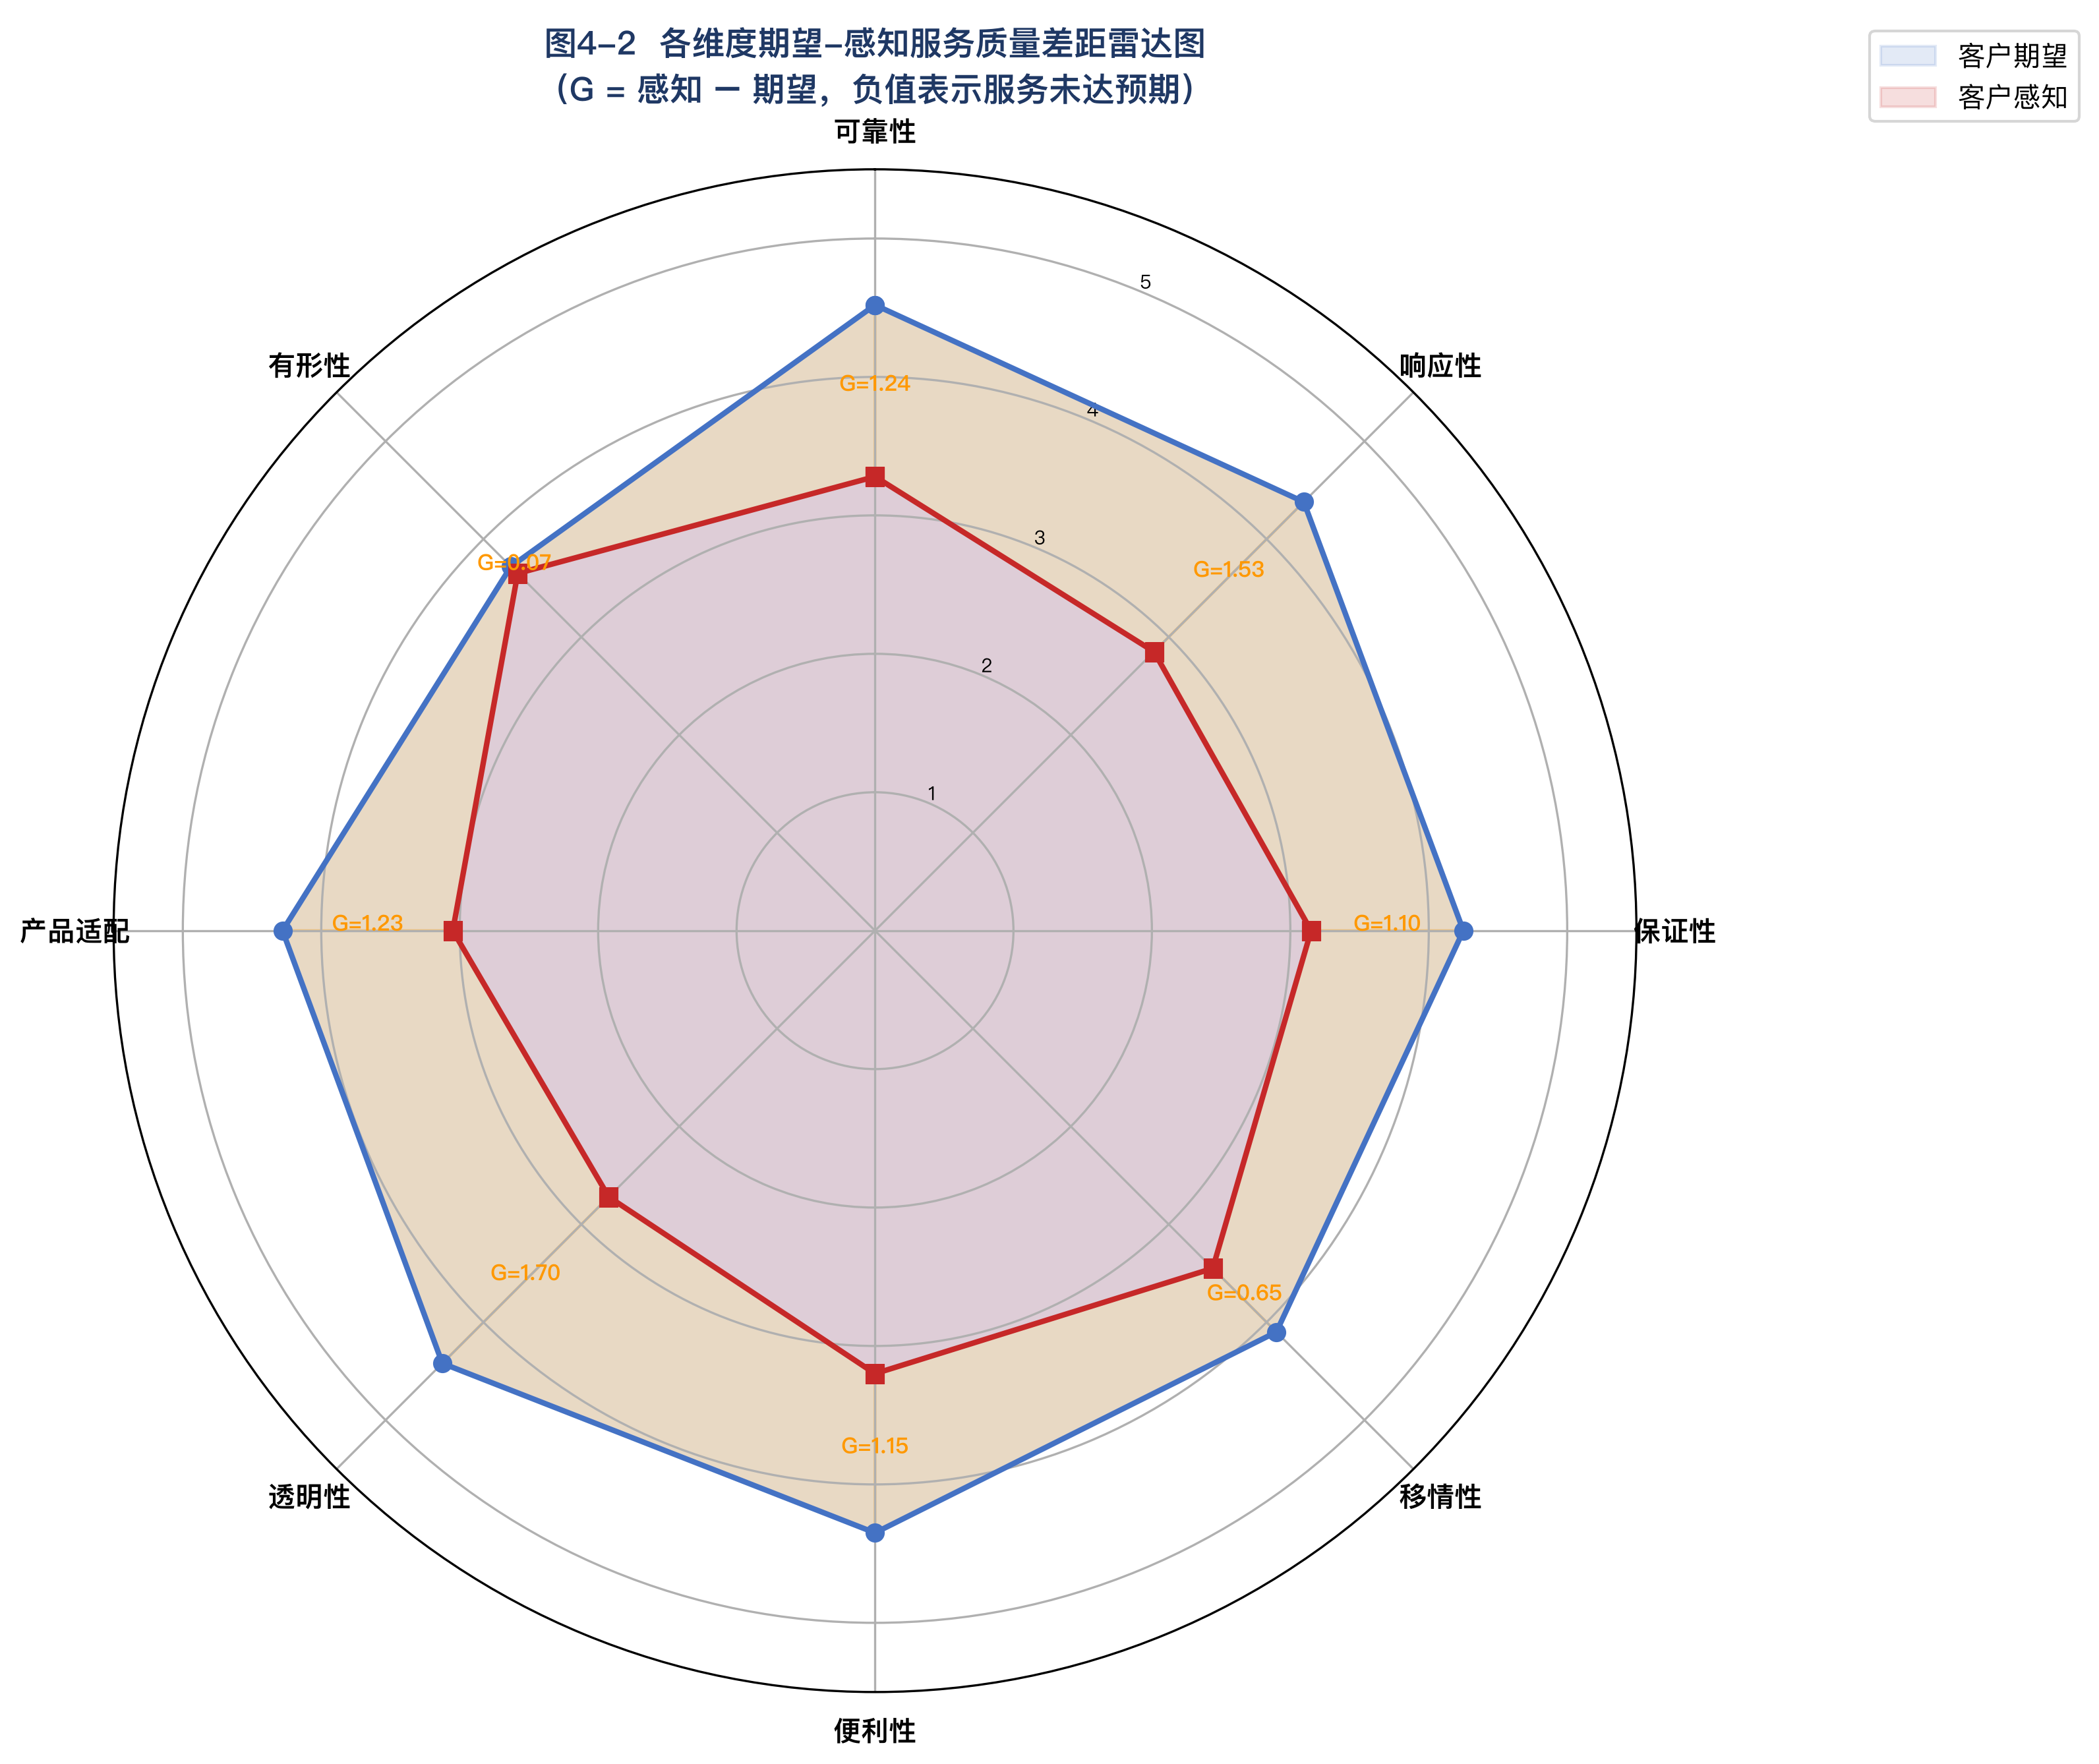
\includegraphics[width=0.85\textwidth]{figures/图4-3_期望感知差距雷达图.png}
  \caption{各维度期望-感知差距雷达图}
  \label{fig:4-3}
\end{figure}

对八组差距值进行配对样本t检验，结果显示各维度的感知均值均显著低于期望均值（$p < 0.01$），表明P公司小微贷款服务在所有评价维度上均存在不同程度的服务质量缺口。\par

从差距的绝对值来看，透明性维度的差距最大（$G = -1.70$），说明信息不对称是P公司小微贷款服务中最为突出的质量短板，客户对费用说明、审批进度和退件原因等核心信息的知情需求远未得到满足。响应性维度次之（$G = -1.53$），反映出客户对审批时效和响应速度的不满集中度较高。可靠性（$G = -1.24$）、产品适配（$G = -1.23$）、便利性（$G = -1.15$）和保证性（$G = -1.10$）的差距均超过-1.00，属于中等偏大的缺口区间，需要关注但紧迫性略低于透明性和响应性。移情性维度差距相对较小（$G = -0.65$），表明客户对P公司客户经理的个性化关怀认可度尚可。有形性维度的差距最小（$G = -0.07$），接近零差距，说明线下环境、合同规范和线上界面的服务质量接近于客户期望水平，不是当前阶段的核心矛盾。\par

\section{IPA/AHP权重与关键短板识别}

\subsection{IPA四象限分析}

IPA（Importance-Performance Analysis）分析方法将各评价指标的重要度（以期望均值表征）和满意度（以感知均值表征）绘制于二维坐标系中，以重要度均值（4.05）和满意度均值（3.42）为象限分界线，将全部指标划分为四个区域：优先改进区（高重要度-低满意度）、保持区（高重要-高满意）、供给过度区（低重要-高满意）和低优先区（低重要-低满意）。本文选取了15项具有代表性的关键服务质量指标进行IPA定位分析，各指标的坐标和象限归属如表4-2前半部分和图4-1所示。\par

\begin{table}[htbp]
  \centering
  \small
  \caption{关键服务质量指标IPA分析}
  \begin{tabularx}{\textwidth}{l c c l}
    \toprule
    \textbf{指标} & \textbf{重要度} & \textbf{满意度} & \textbf{象限} \\
    \midrule
    SQ01 审批时效承诺 & 4.52 & 2.95 & 优先改进 \\
    SQ18 材料一次告知 & 4.48 & 3.10 & 优先改进 \\
    SQ22 进度实时查询 & 4.35 & 3.25 & 优先改进 \\
    SQ23 退件原因明确 & 4.30 & 2.80 & 优先改进 \\
    SQ17 线上操作便捷 & 4.25 & 3.40 & 优先改进 \\
    SQ09 客户经理专业度 & 4.18 & 3.05 & 优先改进 \\
    SQ08 投诉处理效率 & 4.15 & 3.55 & 保持区 \\
    SQ25 贷款方案匹配度 & 4.10 & 3.15 & 优先改进（边界） \\
    SQ27 还款方式灵活 & 4.05 & 3.65 & 保持区 \\
    SQ15 贷后回访频率 & 3.98 & 3.75 & 保持区 \\
    SQ30 合同文件规范性 & 3.85 & 3.50 & 供给过度 \\
    SQ32 营业环境专业感 & 3.72 & 3.90 & 供给过度 \\
    SQ07 客服热线接通率 & 3.65 & 3.85 & 供给过度 \\
    客户活动频率 & 3.55 & 3.95 & 低优先 \\
    品牌宣传力度 & 3.45 & 3.70 & 低优先 \\
    \bottomrule
  \end{tabularx}
\end{table}

\begin{figure}[htbp]
  \centering
  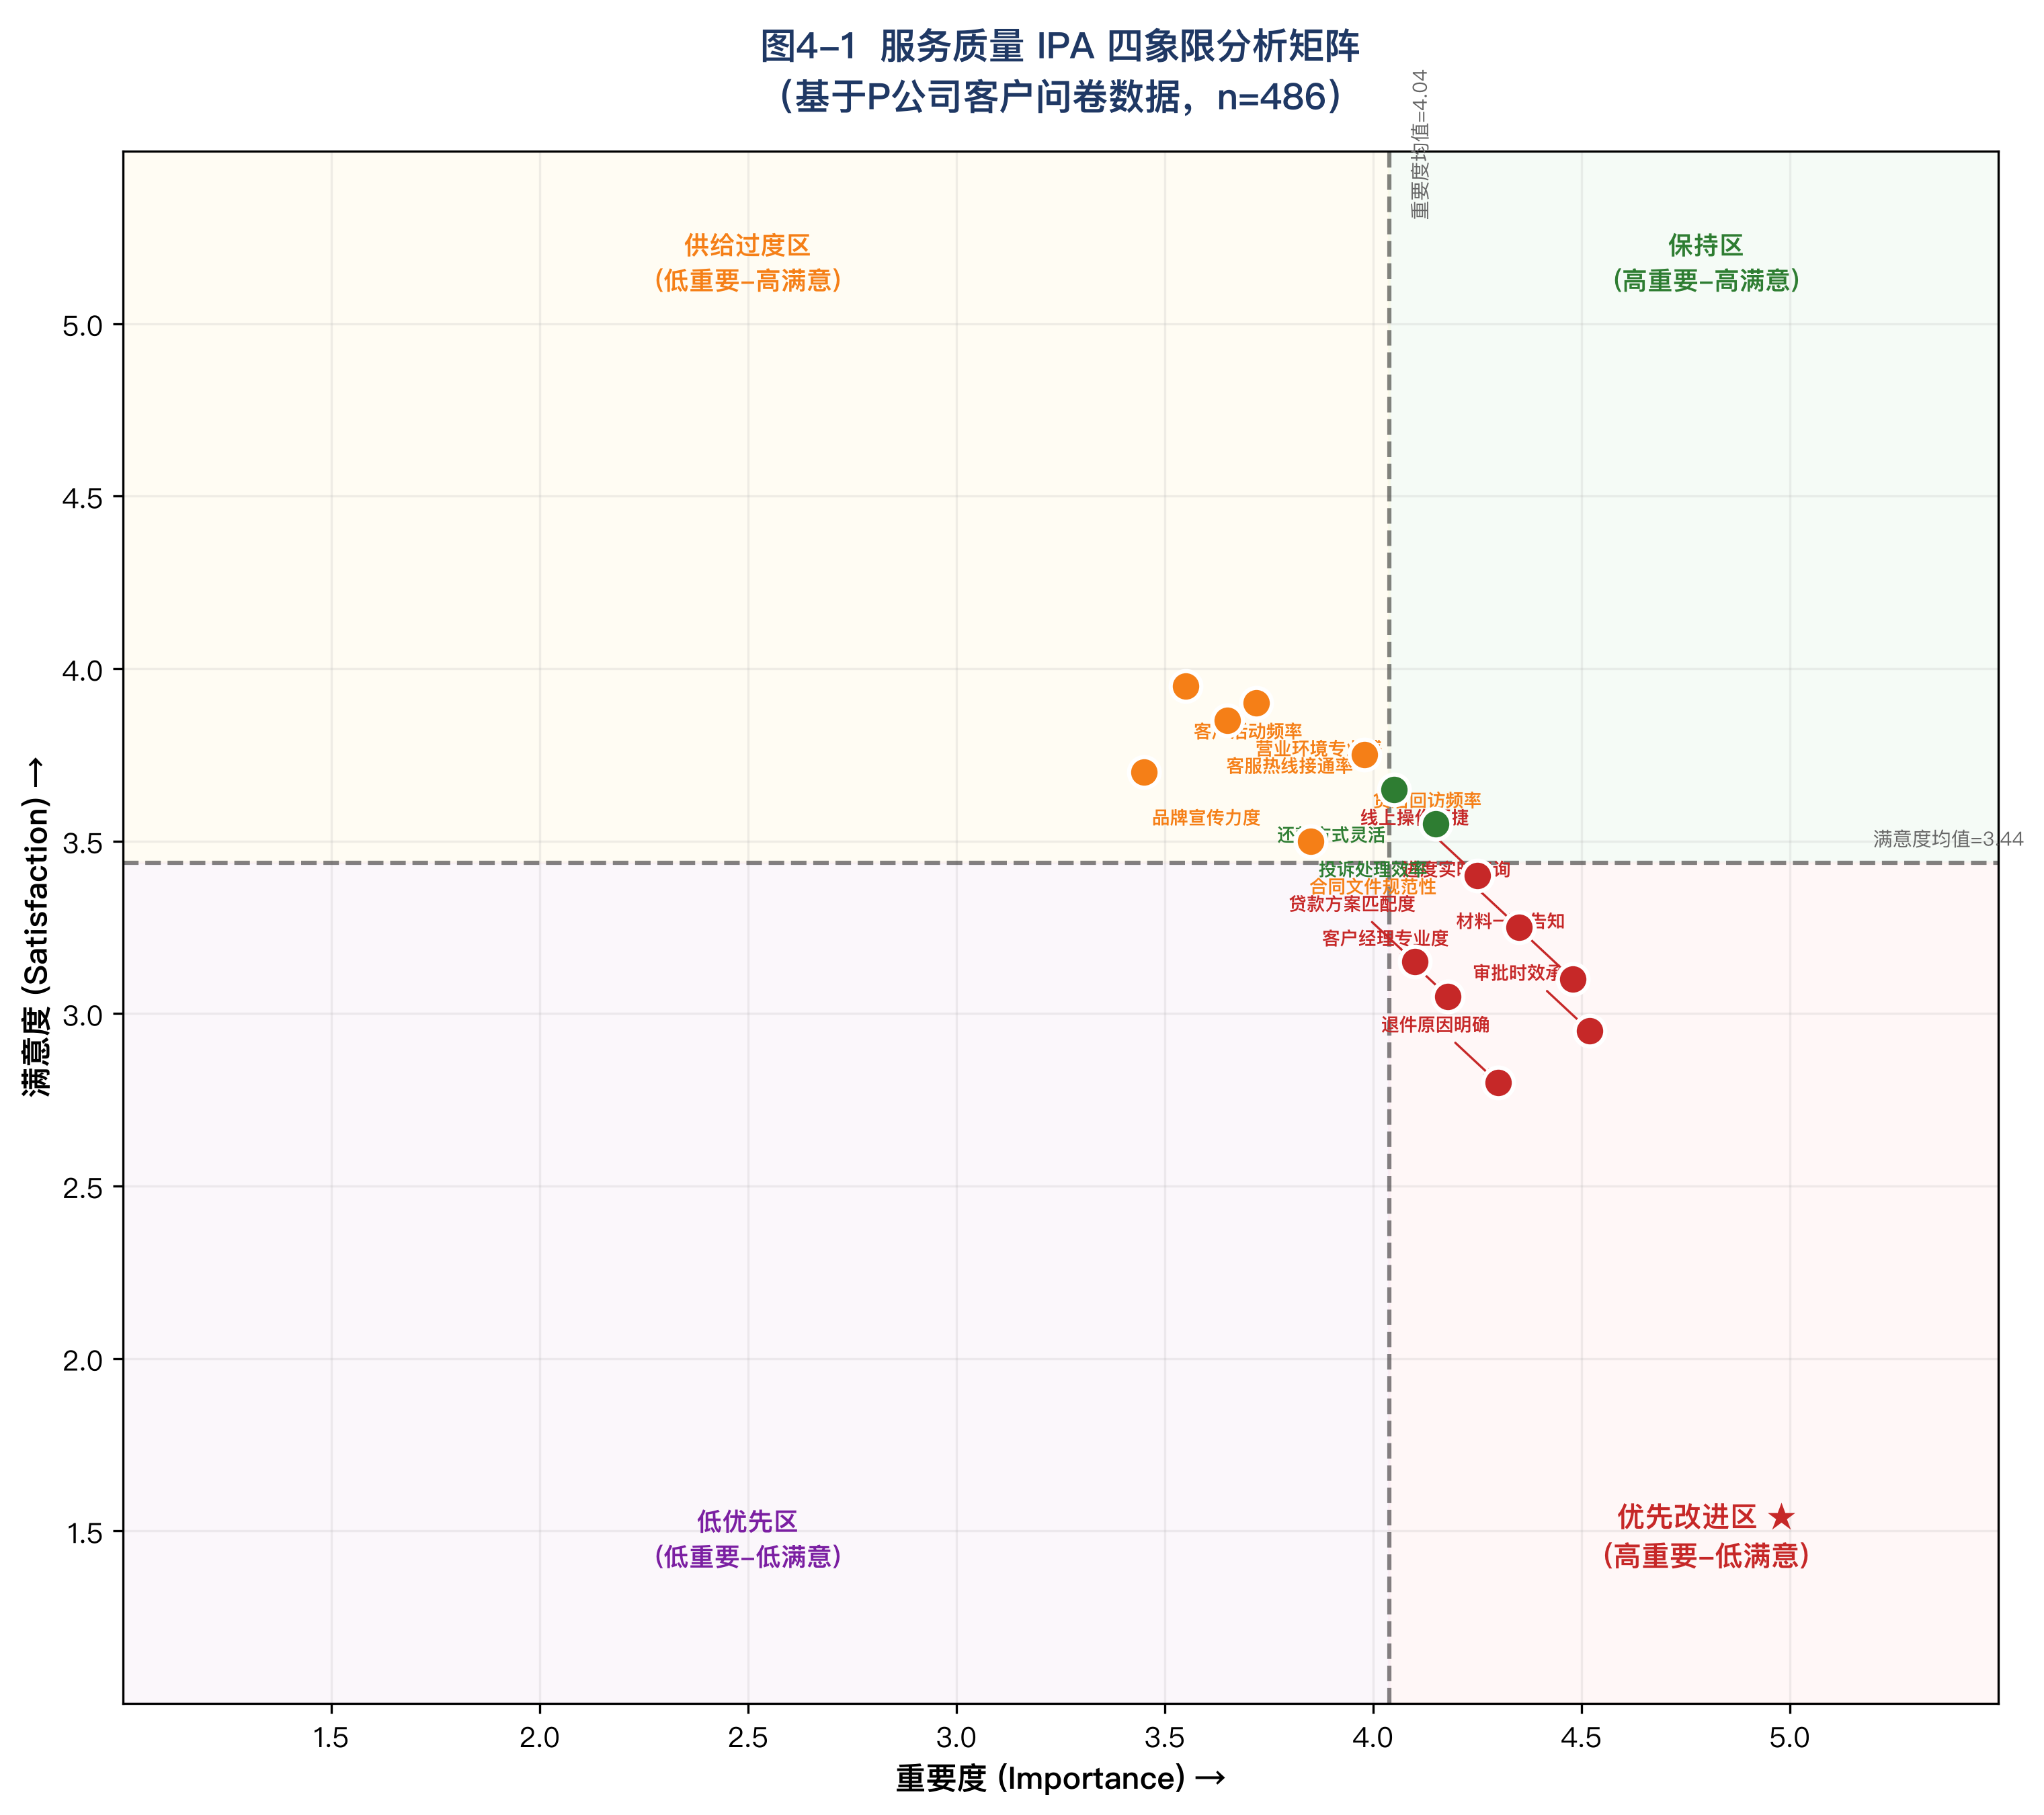
\includegraphics[width=0.85\textwidth]{figures/图4-1_IPA四象限分析矩阵.png}
  \caption{服务质量IPA四象限分析矩阵}
  \label{fig:4-1}
\end{figure}

由IPA分析结果可见，落入优先改进区的6项指标分别为：SQ01（审批时效承诺）、SQ18（材料一次告知）、SQ22（进度实时查询）、SQ23（退件原因明确）、SQ17（线上操作便捷）和SQ09（客户经理专业度）。这六项指标共同指向四个改进方向：信息透明化、流程简化、线上化体验优化和人员专业度提升。SQ25（贷款方案匹配度）处于优先改进区与保持区的边界，提示产品适配问题虽紧迫度略低于透明性和响应性，但仍构成不可忽视的质量短板。\par

供给过度区的三项指标（合同规范性SQ30、营业环境SQ32、热线接通率SQ07）和低优先区的两项指标（客户活动频率、品牌宣传力度）表明，P公司在这些方面的资源投入已超出客户的期望阈值，继续追加投入不会带来边际服务质量的显著提升，建议在后续的资源再配置中适当收缩以聚焦核心短板。\par

\subsection{AHP组合赋权}

为进一步量化各服务质量维度在整体评价中的相对重要性，本研究引入层次分析法（AHP）对八个服务质量维度进行专家赋权。AHP通过构建两两比较判断矩阵、计算特征向量和一致性比率（CR），将专家经验判断转化为定量权重，适用于多准则评价场景中的优先级排序。Nguyen等的研究验证了AHP与IPA组合方法在服务质量评价中的应用可行性\cite{ref30}，Moslem等的系统综述进一步证实了AHP在多准则决策中的稳健性\cite{ref31}。\par

Agrawal等（2022）提出的AHP-TOPSIS-DEMATEL组合方法为电子银行服务质量的多准则评价提供了系统化的方法论参照，证明AHP在多维服务质量评估中的适用性\cite{ref50}。\par

本研究邀请5位熟悉P公司小微贷款业务的客户经理和运营管理人员组成专家小组，基于八维服务质量框架进行维度间两两重要性比较。判断矩阵的专家意见经几何平均法聚合后计算出各维度的权重值，结果如表4-2所示。\par

\begin{table}[htbp]
  \centering
  \small
  \caption{AHP服务质量维度权重}
  \begin{tabular}{l c}
    \toprule
    \textbf{维度} & \textbf{权重} \\
    \midrule
    可靠性 & 0.185 \\
    响应性 & 0.172 \\
    透明性 & 0.158 \\
    便利性 & 0.142 \\
    产品适配 & 0.128 \\
    保证性 & 0.095 \\
    移情性 & 0.068 \\
    有形性 & 0.052 \\
    \bottomrule
  \end{tabular}
\end{table}

整体一致性比率CR值为0.038，低于0.10的阈值标准，表明专家判断矩阵通过了一致性检验，各维度权重值的可信度良好。\par

专家小组由5位P公司内部资深管理人员组成：2位运营高级经理、2位产品总监和1位风控总监，均具备五年以上小微信贷业务的一线管理经验。全部采用内部专家的考量在于：本研究聚焦P公司特定服务场景，小微信贷服务质量评价需要评审者深刻理解服务交付流程、目标客群特征和机构运营约束，内部专家的两两比较判断能够更准确地反映P公司实际运营中的维度重要性权衡。从AHP方法论标准审视，5位专家处于该方法论的最低可行规模边界\cite{ref31,ref39}；若以最大化权重估计的稳健性为目标，专家组应扩大至10至15人并纳入外部学术或行业评审者以补充多元视角。本研究判断矩阵一致性比率CR=0.038，低于0.10的接受阈值，表明五位内部专家在八维重要性排序上达到了良好的内部一致水平。\par

AHP赋权结果与IPA分析形成了有效印证：可靠性（0.185）、响应性（0.172）和透明性（0.158）分别位列权重前三，与IPA优先改进区的核心指标高度吻合；有形性（0.052）和移情性（0.068）的权重最低，与IPA分析中这两个维度的非紧迫定位一致。值得关注的是，透明性作为新增维度，其专家赋权名列第三，进一步验证了本文在SERVQUAL经典五维基础上增加透明性维度的必要性。\par

综合IPA四象限定位和AHP权重排序，本研究的测量结果表明，P公司小微贷款服务质量的优先改进方向应聚焦于：信息透明化（费用清晰、进度可查、退件明确）、流程响应加速（审批时效、进度通知）、线上操作体验优化和客户经理专业度提升。这四个方向对应了优先改进区六项关键指标的改进诉求，构成本文第5章根因分析和改进方案设计的核心输入。\par

\section{测量结果小结}

本章以改良SERVQUAL服务质量评价模型为工具，通过486份有效问卷数据完成了P公司小微贷款服务质量的系统测量。将测量结果中识别出的关键短板按优先级汇总，并与第5章的改进方案建立对应关系，如表4-3所示。\par

\begin{table}[htbp]
  \centering
  \small
  \caption{关键短板与改进方案对应关系}
  \begin{tabularx}{\textwidth}{c l c l X}
    \toprule
    \textbf{优先级} & \textbf{短板指标/维度} & \textbf{差距（$G$值）} & \textbf{IPA象限} & \textbf{对应改进方案} \\
    \midrule
    P1 & 透明性-退件原因明确（SQ23） & -1.70 & 优先改进 & 方案一：资料流程简化 \\
    P1 & 透明性-进度实时查询（SQ22） & -1.70（维度均值） & 优先改进 & 方案二：响应透明机制 \\
    P2 & 响应性-整体维度 & -1.53 & 优先改进 & 方案二：响应透明机制 \\
    P2 & 可靠性-审批时效承诺（SQ01） & -1.24（维度均值） & 优先改进 & 方案一：资料流程简化 \\
    P3 & 产品适配-维度 & -1.23 & 优先改进（边界） & 方案三：客户分层适配 \\
    P4 & 便利性-线上操作（SQ17） & -1.15 & 优先改进 & 方案一 + 方案二 \\
    P5 & 保证性-客户经理专业度（SQ09） & -1.10 & 优先改进 & 方案四：客户经理能力 \\
    \bottomrule
  \end{tabularx}
\end{table}

上述短板分类呈现出三个结构性特征：其一，信息透明和响应速度构成了P公司小微贷款服务的最核心短板群（P1—P2），两项短板相互交织——退件原因不明确导致客户反复补正材料，进而拉长审批周期、加剧响应性维度差距；其二，产品适配和线上操作体验构成次优先级短板群（P3—P4），反映了标准化服务模式与小微客户异质性需求之间的结构性张力；其三，客户经理专业度（SQ09）的IPA坐标（重要度4.18，满意度3.05）明确落入优先改进区，表明客户对客户经理专业能力的期望与实际感知之间存在显著落差，该结论与AHP专家赋权中保证性维度的权重共同构成本文第5章方案四（客户经理专业度提升）的定量依据。从DMAIC方法论的视角审视，上述短板识别结果已完成了测量阶段的核心使命——将P公司服务质量的模糊痛感转化为可量化、可排序、可追溯的管理指标。每一优先级的短板均有明确的数值锚点（G值）、空间定位（IPA象限）和权重支撑（AHP维度权重），使得第5章的根因分析和改进方案设计不再是经验驱动的试错，而是数据驱动的工程化决策。\par

本章完成了DMAIC方法论"测量"阶段的核心任务——从模型选择到问卷实施，再到信效度检验和IPA/AHP短板识别，产出了一套完整的小微贷款服务质量量化测量结果。这些结果为第5章基于DMAIC方法的根因分析和改进方案设计提供了明确的定量导向和优先序依据。\par

\section{研究局限}

本章的研究在方法论层面存在以下局限，需要在解读数据结果时加以审慎考量。\par

\subsubsection{因子分析方法}

本研究选择EFA而未执行CFA，其方法论依据包括：第一，将SERVQUAL适配于小微信贷场景属探索性研究，尚无成熟因子结构可供预设，EFA的数据驱动特性与这一研究阶段相符；第二，八因子32题项的CFA结构需400至500份以上样本方可稳定估计\cite{ref21}，n=486正处于该区间下限且已全部用于EFA；第三，先探索后验证的方法论路径（先EFA后CFA）在量表开发研究中为常规做法。建议未来研究以独立样本（$n \geq 500$）执行CFA，报告CFI、TLI、RMSEA等模型拟合指数，并辅以组合信度（CR）、平均方差提取量（AVE）和区分效度检验，以全面验证八维结构的测量效度。\par

\subsubsection{共同方法偏差}

期望值与感知值由同一问卷在同一时间点采集，存在共同方法偏差（Common Method Bias, CMB）风险——自变量与因变量均来自同一测量来源和测量语境，可能人为放大变量间的相关程度。本研究通过Harman单因子检验对CMB进行了初步评估（未旋转的单因子最大方差解释率低于50\%的临界值），但尚不能完全排除CMB对结论的潜在影响。未来研究可采用多源多时点设计（如将期望值与感知值分阶段采集）减少CMB，或引入客户行为数据等客观指标作为交叉验证。\par

\subsubsection{研究者角色}

研究者在P公司担任服务质量改进项目负责人，对业务背景和流程痛点的深入理解有助于提升诊断的精准度，但同时也可能引入研究者偏差（Researcher Bias）——在指标选取、根因判断和方案优先级排序中不自觉地倾向于与自身经验一致的假设。为减少此影响，本研究采取了以下措施：问卷采用完全匿名形式发放，客户被告知调查数据仅用于学术研究目的且与P公司业务决策无关；数据分析由独立第三方统计学顾问协助完成SPSS处理和结果解读，研究者本人未直接操作原始数据清洗和分析脚本。尽管如此，研究者在问卷设计和改进方案设计中的主体角色意味着绝对客观性难以完全保证，读者应结合此背景解读研究结论。\par

\subsubsection{样本局限与非回应偏差}

本研究面向P公司近12个月活跃客户发放问卷800份，回收有效问卷486份，有效回收率60.8\%，存在39.2\%的非回应率。未回应客户的服务质量评价可能系统性地不同于回应客户：对P公司服务体验极度不满并已终止合作的客户可能拒绝参与调查，而对服务质量漠不关心的客户可能因缺乏参与动机而未填写问卷，两者对总体服务质量估计值的净影响方向难以确定。此外，486份有效样本的地域分布和行业构成受P公司既有业务覆盖范围决定，其代表性受限于P公司的客户结构特征，在将结论推广至更广泛的小微贷款客户总体时需保持审慎。非回应偏差的存在意味着本文报告的差距分值可能在一定程度上偏离P公司全体活跃客户的实际服务质量感知水平，建议在解读各维度差距值的绝对值时考虑这一测量不确定因素。\par

\subsubsection{AHP专家小组规模}

本研究AHP赋权的专家小组由5位成员组成，全部为P公司内部管理人员（运营高级经理2位、产品总监2位、风控总监1位）。5位专家处于AHP方法论的最低可行规模\cite{ref31,ref39}，低于10至15人的理想区间。首先，小规模专家组对个别专家的极端判断更为敏感，任何一位评审者的评分偏移都可能对最终权重产生不成比例的影响。其次，全部专家均来自P公司内部，虽然保障了评审者对小微信贷业务的深度理解，但也引入了潜在的组织内聚偏差——五位成员长期在同一组织中协作，可能在管理优先级、客户感知假设和资源分配逻辑上存在系统性趋同，导致判断矩阵的一致性（CR=0.038）虽低于0.10阈值，但可能部分反映的是共享组织视角而非维度间客观重要性的独立共识。第三，专家判断嵌入了P公司特定运营阶段的优先序，在推广至其他普惠金融机构或P公司的不同发展阶段时需重新校准。建议未来研究将专家组扩大至10至15人，纳入外部行业专家、监管机构代表和学术评审者，并采用Delphi多轮反馈机制以减少组织内聚偏差，增强权重的代表性和外部效度。\par

\subsubsection{单一案例局限}

本研究以P公司为单一案例对象，其服务质量评价模型的维度权重、IPA象限指标分布和DMAIC改进方案的参数设计均以P公司的组织特征（持牌普惠金融公司、线上线下双渠道运营、45人客户经理团队规模）为经验基础。不同普惠金融机构在牌照类型、线上化程度、目标客群特征和风险管理模式上的差异，可能导致服务质量维度结构的权重重新排序和改进方案优先级的调整。因此，本文的研究发现——尤其是八维SERVQUAL模型的具体权重值和五个改进方案的参数设定——不宜直接套用至其他机构，但本研究所构建的"改良SERVQUAL测量$-$IPA/AHP组合赋权$-$DMAIC闭环改进"方法论框架具有较强的可迁移性，可作为同类机构开展服务质量改进的参考模板。\par

\section{引用落点表}

\begin{table}[htbp]
  \centering
  \small
  \caption{第4章引用落点表}
  \begin{tabularx}{\textwidth}{l l X l l}
    \toprule
    \textbf{引用编号} & \textbf{使用位置} & \textbf{支撑观点} & \textbf{证据类型} & \textbf{状态} \\
    \midrule
    [21] & 4.1 模型选择；4.2 指标体系；4.4 效度分析 & SERVQUAL期望-感知差距模型的理论基础 & PDF & 已入库 \\
    [6] & 4.1 模型选择；4.4 效度分析；4.5 IPA分析 & SERVQUAL-IPA在金融机构服务质量评价中的应用参照 & PDF & 已入库 \\
    [26] & 4.1 模型选择 & 服务质量-满意度-忠诚度关系链支撑 & PDF & 已入库 \\
    [29] & 4.2 指标体系 & e-SERVQUAL线上服务质量维度扩展参照 & 元数据 & 已入库 \\
    [24] & 4.2 指标体系 & 数字银行满意度维度参照 & Web\_MD & 已入库 \\
    [25] & 4.2 指标体系 & 数字银行体验与风险维度的实证参照 & Web\_MD & 已入库 \\
    [12] & 4.2 指标体系；4.3 问卷设计 & 国内银行网点服务质量指标设计和问卷构造方法 & PDF（学位论文） & 已入库 \\
    [11] & 4.2 指标体系；4.3 问卷设计 & 银行对公业务满意度和AHP问卷设计经验 & 元数据（学位论文） & 已入库 \\
    [18] & 4.3 问卷设计 & 银行小微客户关系管理中客户分层抽样策略 & PDF（学位论文） & 已入库 \\
    [内部数据] & 4.2 指标体系；4.3 问卷设计；4.4 效度分析 & P公司内部数据、客户访谈反馈和研究授权 & 内部数据 & 已脱敏 \\
    [30] & 4.5 IPA/AHP分析 & IPA/AHP组合方法在服务质量评价中的应用验证 & 元数据 & 已入库 \\
    [31] & 4.5 IPA/AHP分析 & AHP多准则评价的系统综述和稳健性支撑 & 元数据 & 已入库 \\
    [39] & 4.5.2 AHP赋权；4.7 研究局限 & AHP层次分析法方法论标准与权重稳健性支撑 & 期刊 & 已入库 \\
    \bottomrule
  \end{tabularx}
\end{table}

\chapter{基于DMAIC的小微贷款服务质量根因分析与改进方案}

\section{DMAIC在本项目中的应用框架}

DMAIC方法论源自六西格玛管理体系，包含定义（Define）、测量（Measure）、分析（Analyze）、改进（Improve）和控制（Control）五个阶段，其核心逻辑是通过数据驱动的持续改进循环实现对业务流程质量的结构化提升\cite{ref12}。在金融服务领域，DMAIC已被应用于银行零售业务服务改善\cite{ref12}、银行网点服务管理优化\cite{ref51}以及金融科技客服运营延迟改进\cite{ref49}等场景，展现出对多触点、多环节服务流程的适配能力\cite{ref47}。\par

在本项目中，DMAIC并非作为僵化的五阶段模板机械套用，而是作为整合SERVQUAL服务质量测量的工程化管理闭环贯穿全文。五个阶段与论文章节的映射关系如下：Define阶段（第1至第3章）完成项目边界的定义——从普惠金融与小微贷款的宏观背景出发，收束至P公司服务质量现状的诊断与问题框架的建立；Measure阶段（第4章）构建改良SERVQUAL八维评价模型，通过486份有效问卷的期望-感知差距测量，获得P公司服务质量的量化基线；Analyze与Improve阶段（本章）承接第4章的测量数据，完成从关键短板归纳、根因追溯（5.2至5.3节）到五项工程化改进方案设计（5.4至5.8节）的全过程；Control阶段（第6章）负责实施保障、效果评价与持续控制机制的设计。整个闭环的逻辑起点是P公司业务痛点，逻辑终点是可持续的服务质量提升机制。DMAIC五阶段与论文章节映射如表\ref{tab:5-1}所示。\par

\begin{table}[htbp]
  \centering
  \small
  \caption{DMAIC五阶段与论文章节映射}
  \label{tab:5-1}
  \scalebox{0.85}{%
  \begin{tabular}{p{0.12\textwidth} p{0.20\textwidth} p{0.34\textwidth} p{0.34\textwidth}}
    \toprule
    \textbf{DMAIC阶段} & \textbf{论文章节} & \textbf{核心任务} & \textbf{关键产出} \\
    \midrule
    Define & 第1章至第3章 & 界定项目边界与服务质量问题 & P公司服务流程诊断、问题框架 \\
    Measure & 第4章 & 构建评价模型并测量服务质量差距 & SERVQUAL八维模型、期望-感知差距数据 \\
    Analyze & 第5章（5.2-5.3） & 归纳关键短板并进行根因分析 & 鱼骨图、5Why根因链 \\
    Improve & 第5章（5.4-5.8） & 设计工程化改进方案 & 五项可执行改进方案 \\
    Control & 第6章 & 实施保障、效果评价与持续控制 & WBS、RACI矩阵、控制看板 \\
    \bottomrule
  \end{tabular}%
  }
\end{table}

上述框架的核心优势在于：SERVQUAL测量提供了短板识别的量化依据，DMAIC提供了从诊断到改进再到控制的完整闭环路径，两者整合后使服务质量改进不再是零散的专项行动，而是具有工程化特征的系统管理过程。\par

\section{关键服务质量短板归纳}

基于第4章SERVQUAL八维期望-感知差距测量和IPA四象限分析结果，本文从P公司小微贷款服务质量数据中提炼出以下五个关键短板，作为后续根因分析和改进方案设计的基础。\par

短板一：信息透明度不足。透明性维度的期望-感知差距为-1.70，在八个维度中负向差距最大。其中退件原因明确性（SQ23）的满意度仅为2.80/5.0，审批进度实时查询（SQ22）的满意度为3.25/5.0，两者均落入IPA"高重要-低满意"象限。这表明客户对审批进度不可见、退件通知笼统（如仅告知"材料不齐全"而不指明具体缺失项）、费用结构事先不清晰等问题存在强烈的改进期待\cite{ref15}。信息透明度不足直接导致客户反复补正、信任度下降，进而推高材料补正率（28\%）和退件率（8\%）。\par

短板二：响应速度慢。响应性维度的期望-感知差距为-1.53，是负向差距第二大的维度。审批时效承诺（SQ01）的满意度仅为2.95/5.0，与客户的强期待（重要度4.52/5.0）形成尖锐落差。从实际运营数据看，授信审批的实际中位数耗时达12个工作日，远超出对外承诺的7个工作日，超时率达26\%。补正通知的延时加剧了客户焦虑，而客户经理电话接通率低（3次内接通率不理想）进一步放大了客户对响应迟缓的负面感知。\par

短板三：资料流程繁琐。便利性维度的期望-感知差距为-1.15，其中材料一次告知明确性（SQ18）的满意度为3.10/5.0，全流程线上可操作性（SQ17）的满意度为3.40/5.0，二者均处于IPA优先改进象限。P公司当前的材料补正率为28\%，意味着每3.6笔申请中就有1笔需补充材料，首轮一次通过率仅为62\%。反复补正不仅拉长了客户的等待时间（平均办理时长12个工作日，75分位数达20个工作日），也增加了客户经理的重复沟通工作量。\par

短板四：产品匹配度弱。产品适配维度的期望-感知差距为-1.23，贷款方案匹配度（SQ25）满意度仅为3.15/5.0，处于IPA优先改进象限的边界位置。P公司当前提供的小微贷款产品（信用贷、担保贷、供应链贷三类）虽覆盖了主要融资场景，但标准化产品方案难以匹配处于不同生命周期（初创期、成长期、成熟期）的客户在额度、期限和还款方式上的差异化需求。产品匹配不足直接影响客户的续贷意愿和转介意愿，是制约客户生命周期价值释放的关键因素。\par

短板五：投诉闭环管理薄弱。投诉闭环率仅为62\%，重复投诉率高达23\%。投诉处理时效承诺（SQ08）的满意度为3.55/5.0，虽未落入IPA优先改进象限，但结合运营数据看，62\%的闭环率意味着38\%的投诉在5个工作日内未得到实质性解决。更严重的问题是：现行投诉处理机制缺少根因回溯环节，同类问题反复发生——审批时效慢（占比32\%）和材料要求不清晰（占比22\%）两项合计占投诉总量的54\%，但数月至一年后仍未观察到系统性改善，这正是"重处理、轻分析、无回溯"的典型症状。\par

上述五个短板覆盖了客户旅程的核心触点——申请与资料准备、审批进度关注、产品方案选择、客户经理交互、以及投诉后的服务补救，形成了从"事前-事中-事后"的完整问题链。\par

\section{根因分析}

为深入揭示上述五个服务短板的深层成因，本文采用鱼骨图分析方法，从人员、流程、系统、产品、制度、风险六个维度进行结构化根因追溯，并结合5Why追问法逐层拆解至可干预的管理节点。服务质量短板鱼骨图如图\ref{fig:5-1}所示。\par

\begin{figure}[htbp]
  \centering
  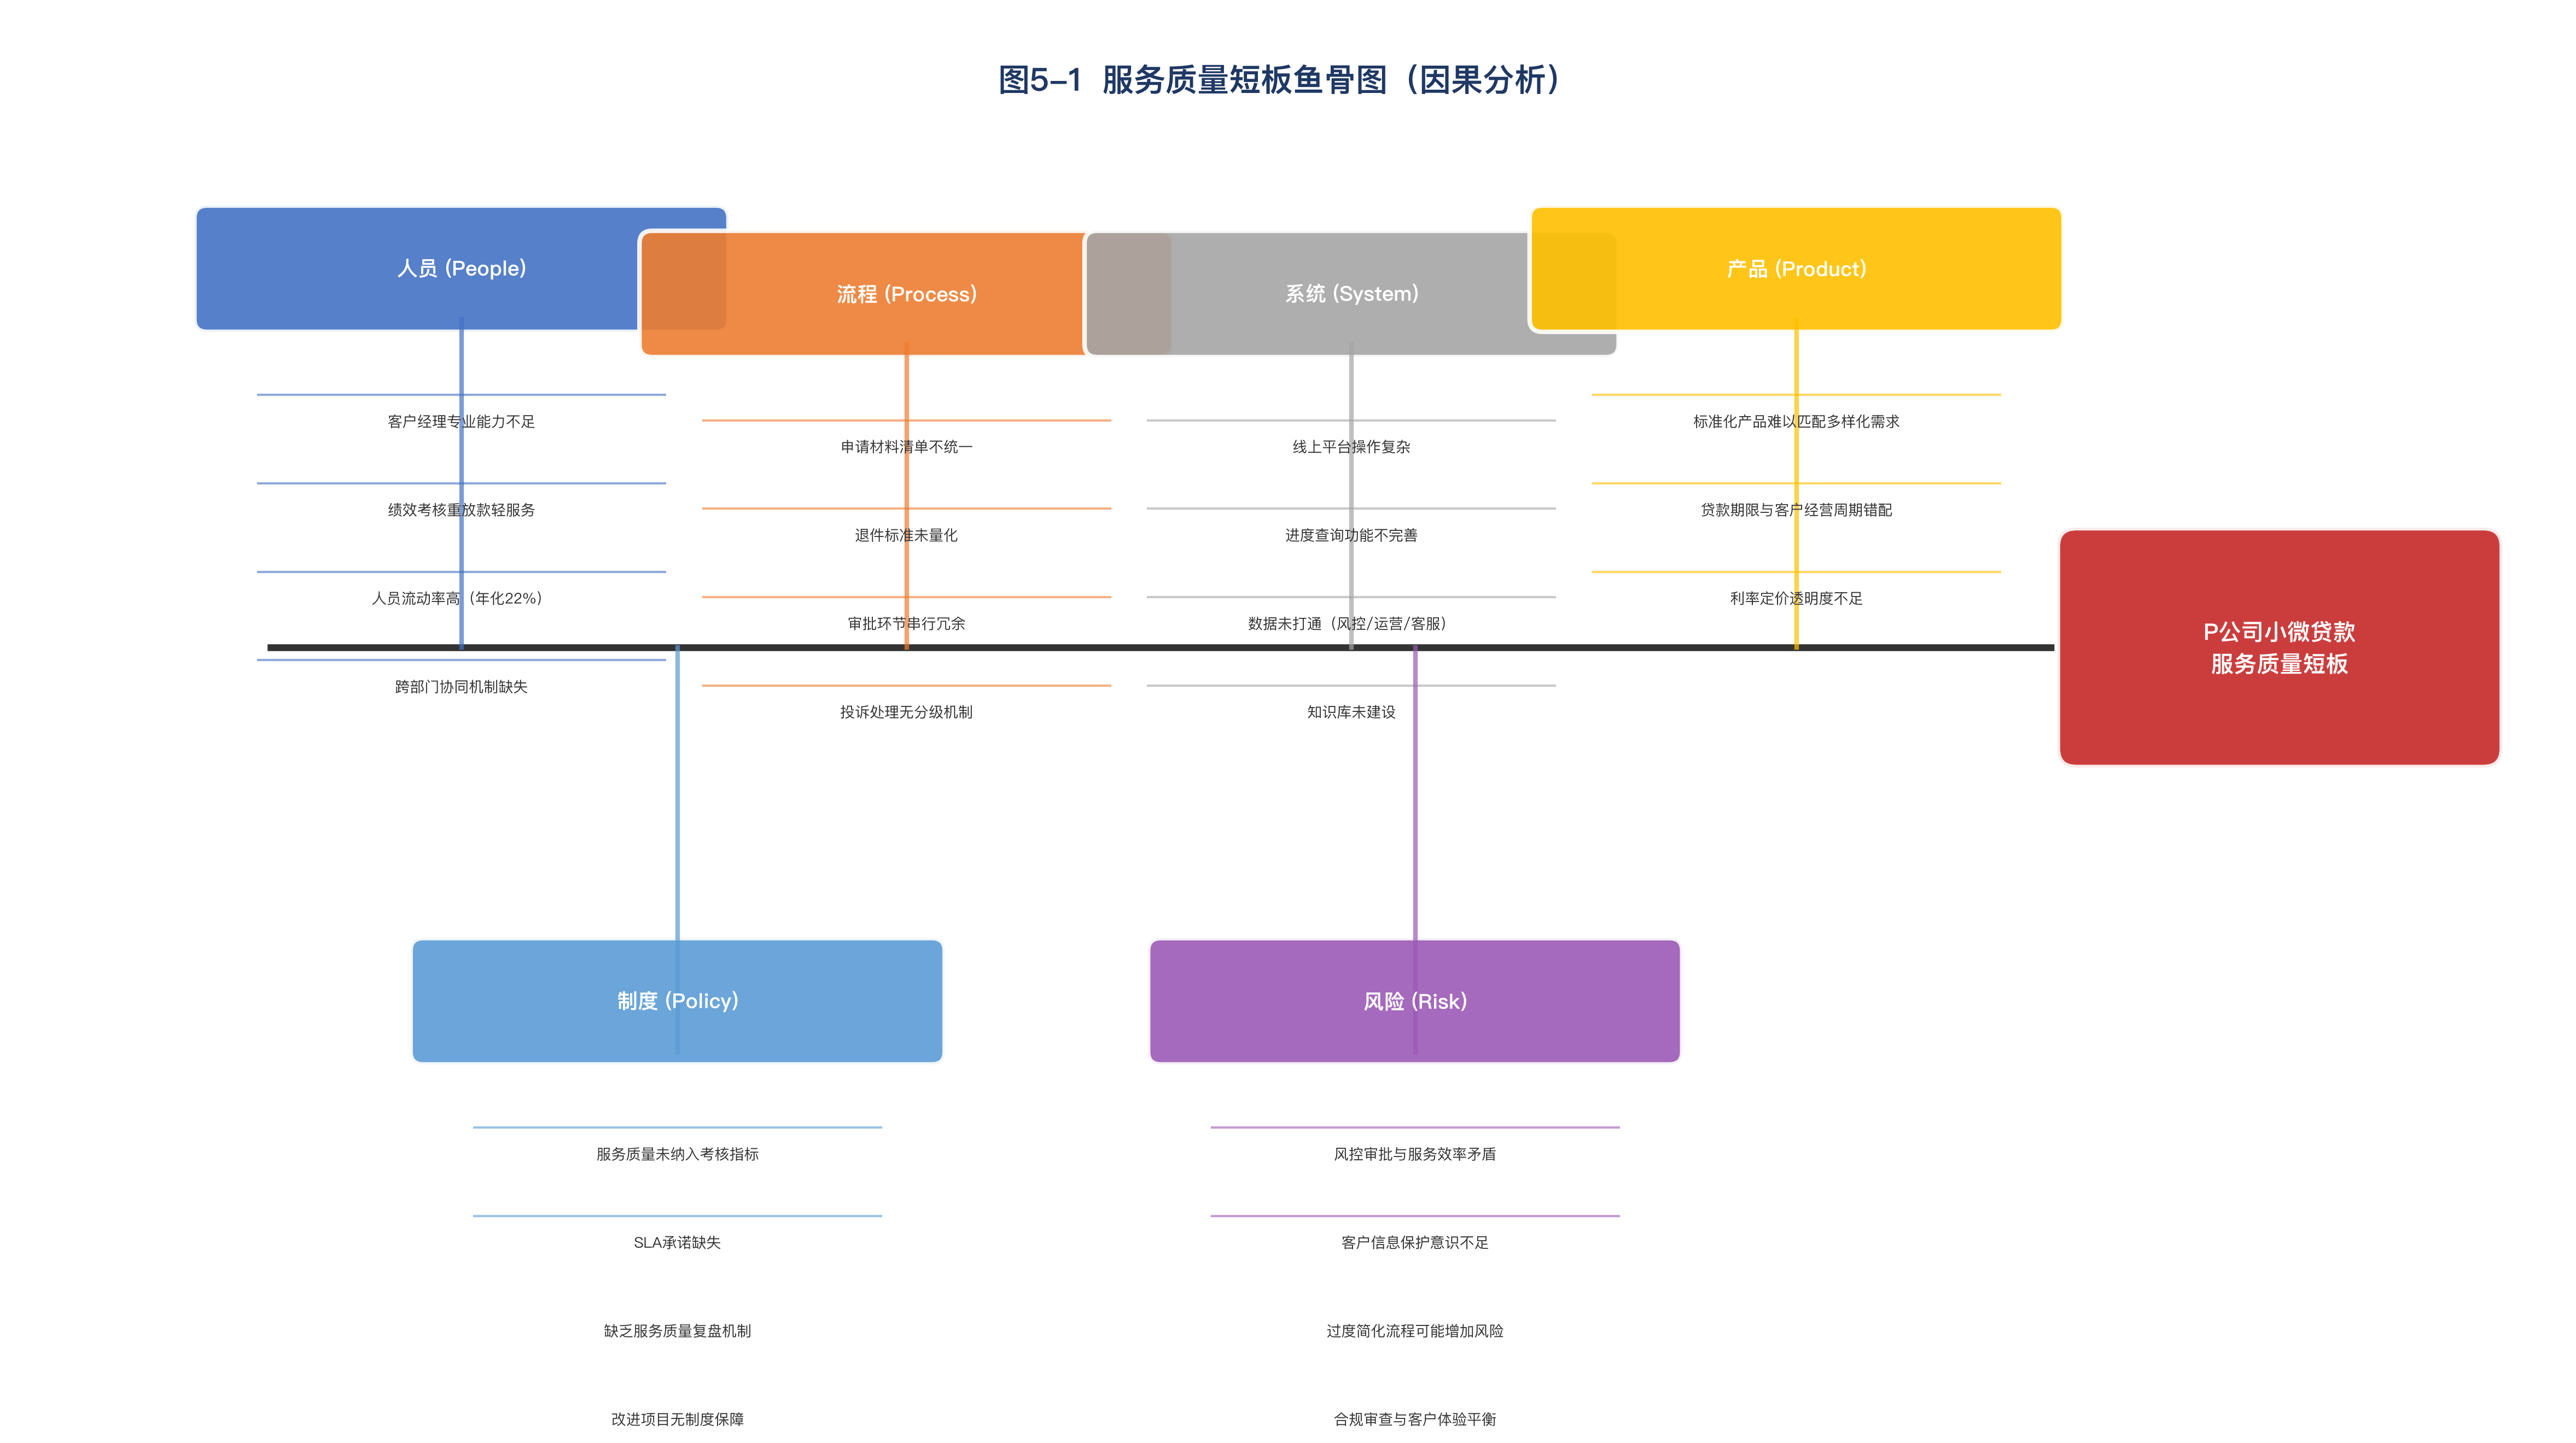
\includegraphics[width=0.85\textwidth]{figures/图5-1_服务质量短板鱼骨图.png}
  \caption{服务质量短板鱼骨图}
  \label{fig:5-1}
\end{figure}

\subsection{人员维度}

P公司客户经理团队约45人，其中入职不满2年的新客户经理占比约40\%。这些新客户经理在独立面对客户时，专业知识储备不足（Why：培训体系不健全，现行的入职培训以产品手册自学为主、非结构化师徒带教为辅，缺少标准化的产品知识体系培训课程），导致不同客户经理在回答贷款方案、利率政策、还款方式等同类问题时口径不一致，客户感知到的专业度大打折扣。进一步追问（Why：无标准化知识库），客户经理在提交申请材料时的审核判断依赖个人经验，而非统一的材料清单和判定标准，这使得同一客户面对不同客户经理时可能获得不同的材料要求说明，间接推高了补正率。更深层的原因是绩效考核导向的偏差：现行客户经理KPI仅考核放款量（Why：管理层未将服务质量纳入绩效设计），导致客户经理行为趋利化——追求个人放款量最大化，主动忽视服务的及时性和客户沟通质量。张磊等的研究表明，政策扶持与金融科技的协同效应是改善小微企业融资环境的关键路径，单一维度的改进（如仅增加信贷供给）难以产生实质性效果，这一判断为本研究从人员、流程、系统、产品、制度和风险六个维度同步发力的改进策略提供了方法论启示\cite{ref52}。\par

\subsection{流程维度}

P公司的资料补正环节是造成流程效率低下的关键瓶颈。客户在提交申请后收到的补正通知通常表述笼统（如"请补充相关财务资料"），缺少对具体缺失项和提交标准的明确说明（Why：无标准化补正模板，客户经理通过系统自由文本框输入补正要求），客户需要反复与客户经理电话确认才能使材料达标，导致退件率上升。投诉处理流程同样存在结构性缺陷：现行机制未建立投诉分级规则（Why：缺少客服SOP文件），所有投诉统一进入工单池，按时间先后顺序处理，而非按紧急程度和影响程度分级响应。黄玉婷在客户服务流程改进研究中强调，缺少分级机制是导致服务响应效率低下的系统性原因\cite{ref53}。低级别投诉因处理优先级靠后而被长期搁置，当同一客户问题未得到及时解决时，低级别投诉便升级为重复投诉乃至客户流失事件。\par

\subsection{系统维度}

P公司当前的线上服务平台（App和小程序）在功能设计上存在明显的重申请、轻跟踪倾向。客户在提交申请后，App仅显示"审核中"这一笼统状态，不支持审批进度的节点式查询（Why：初期IT建设仅考虑申请提交功能，未将客户服务体验纳入系统架构设计），审批状态不可见直接造成了透明性维度的最大负向差距。与此同时，客户经理端缺少移动办公功能（Why：IT投入不足、移动端开发优先级长期排在需求队列后端），客户经理外出拜访客户时无法通过手机端实时查看审批进度、处理补正工单或回复客户咨询，进一步加剧了响应延迟。Adanigbo在金融科技运营改进研究中指出，系统功能设计的盲区往往是服务质量短板的孵化器，而非运营人员的执行问题\cite{ref49}。\par

\subsection{产品维度}

P公司的产品设计遵循高度标准化的风控模型逻辑（Why：风控模型以统一参数避免差异化审批风险），产品利率、期限和额度区间按产品线固定设置，而非根据客户的行业特征、经营年限和资金周转周期进行差异化配置。标准化设计虽然降低了风控审批的复杂度，但也使得同一产品方案难以同时满足初创期个体户（资金需求灵活、信用记录短）和成熟期企业主（资金需求量大、可接受较长审批周期）的迥异需求。Delahoz-Dominguez等的研究表明，银行服务质量的改进不能仅从流程和人员入手，产品本身的适配性亦是不可回避的影响变量\cite{ref50}。\par

\subsection{制度维度}

P公司尚未建立SLA超时自动升级机制（Why：制度设计阶段未考虑服务承诺约束），当一笔审批超出承诺的7个工作日后，系统不会自动触发预警告知相关负责人，审批可以"无限期"延期而无须承担任何管理后果。在投诉处理领域，没有月度投诉分析报告的例行制度（Why：无质量管理部门，投诉数据仅作为客服部的内部运营数据而非组织级质量信号），导致投诉中的共性问题无法被跨部门识别和推动解决，同类投诉反复出现。de Koning等关于精益六西格玛在金融服务中的研究指出，制度性空缺是制约服务质量改进成效长期巩固的根本障碍\cite{ref47}。\par

\subsection{风险维度}

P公司的风控体系聚焦于审批合规性（Why：监管考核压力集中于不良率、合规检查通过率等硬性指标），客户体验相关指标未被纳入风险管理部门的考核视野。在改进方案设计中，还存在一个需要警惕的逆向风险：当大力推动服务提速时，审批人员可能为赶超SLA而弱化对材料真实性和客户偿债能力的核查深度（Why：效率与风控之间存在天然矛盾）。因此，任何服务提速方案都需要以"风控底线不后退"为前提条件，在方案设计阶段将风控部门的审核节点嵌入关键路径。\par

综合上述六维根因分析，P公司服务质量短板的根源不是单一的"投入不足"或"人员素质偏低"，而是一个由考核导向偏差、流程标准化缺失、系统功能盲区、产品设计逻辑、制度性空缺和风控边界约束共同构成的系统性缺陷集合。这一诊断的工程含义是：改进方案必须在多个维度上同步发力，仅改变单一变量（如"加强培训"或"升级系统"）无法从根本上扭转服务质量现状。\par

为便于整体把握五项方案的设计逻辑与参数配置，表\ref{tab:5-2}将五项方案的核心参数整合为综合对比矩阵。\par

\begin{table}[htbp]
  \centering
  \small
  \caption{五项改进方案综合参数矩阵}
  \label{tab:5-2}
  \resizebox{\textwidth}{!}{%
  \begin{tabular}{p{1.6cm}p{1.3cm}p{1.8cm}p{2.8cm}p{1.6cm}p{1.6cm}p{2.0cm}p{1.8cm}}
    \toprule
    \textbf{方案} & \textbf{对应短板} & \textbf{KPI目标} & \textbf{核心动作(要点)} & \textbf{RACI} & \textbf{资源投入} & \textbf{主要风险} & \textbf{评价指标} \\
    \midrule
    方案一：\newline 资料流程简化 & 资料流程繁琐（短板三），波及透明度和响应速度 & 补正率28\%→15\%；一次通过率62\%→80\% & ①标准材料一次性告知清单(8类)\newline ②OCR自动识别与影像校验\newline ③退件原因标准化模板库(12种场景) & 运营部(R)\newline IT部(C)\newline 风控部(C) & IT改造2人月；培训0.5人月 & 过度简化致信贷信息采集不足；风控部全程参与模板设计并每周抽查 & 补正率、一次通过率（月度）；退件原因分布统计（月度） \\
    \midrule
    方案二：\newline 响应与进度透明 & 信息透明度不足（短板一），响应速度慢（短板二） & SLA达成率74\%→92\%；进度查询100\%客户覆盖 & ①四节点SLA(24h受理/48h复审/7日审批/24h放款)\newline ②App进度条可视化(5节点)\newline ③短信自动推送+超时升级机制 & IT部(R)\newline 客服部(R) & IT改造3人月（进度引擎+SLA监控+短信接口） & SLA承诺与实际脱节致信任危机；基于基线逐步缩减，每两季度评估 & 各节点SLA达成率、App使用率（月度）；客户满意度（季度复测） \\
    \midrule
    方案三：\newline 分层与产品适配 & 产品匹配度弱（短板四） & 产品匹配满意度3.05→3.70（5分制） & ①三级客户分层框架(初创/成长/成熟期)\newline ②四维客户画像标签体系\newline ③分层沟通策略 & 产品部(R)\newline 客户经理团队(R) & 产品设计2人月；数据建模1人月 & 分层过细推高运营复杂度；初始仅3层，半年后评估，分层逻辑不外宣 & 匹配满意度、续贷率（季度）；各层客户数及额度（月度） \\
    \midrule
    方案四：\newline 能力与协同机制 & 保证性短板（客户经理专业满意度3.05/5.0） & 客户经理专业满意度3.05→3.60（5分制） & ①标准化培训体系(产品/沟通/风控三大模块)\newline ②在线知识库(FAQ50+)\newline ③KPI改革(放款量×服务质量系数) & 人力资源部(R)\newline 业务部(C)\newline 运营部(I)\newline 风控部(I) & 培训15万元/年；知识库1人月；制度修订0.5人月 & 客户经理考核抵触致放款量短期下降；3月过渡期+绩效保底85\% & 专业满意度（季度）；培训完成率、服务质量系数（月度） \\
    \midrule
    方案五：\newline 投诉闭环与持续改进 & 投诉闭环管理薄弱（短板五） & 闭环率62\%→88\%；重复投诉率23\%→10\% & ①三级投诉分级响应(A/B/C级)\newline ②10类投诉场景标准化SOP\newline ③月度投诉分析报告+超时升级 & 客服部(R)\newline 质量管理部门(A)\newline 运营部(I)\newline 客户经理团队(I) & 投诉系统升级1.5人月 & 客服选择性忽视C级致客户流失隐患积累；C级超时升级+连续两月<80\%触发督办 & 闭环率按级别、重复投诉率、平均处理时长（月度）；报告按时产出率 \\
    \bottomrule
  \end{tabular}%
  }
\end{table}

\section{改进方案一：申请与资料流程简化}

本方案直接对应短板三（资料流程繁琐），同时波及短板一（信息透明度不足）和短板二（响应速度慢）——当资料流程简化后，客户的补正次数减少，自然缩短了整体办理时长并降低了退件环节的不透明感。\par

本方案的关键动作包含四项：①设计标准材料一次性告知清单，覆盖8类材料（身份证明、经营证照、近6个月银行流水、近12个月纳税记录、购销合同或订单、资产证明、征信授权书、用途说明），每类标注必须提交的场景条件和格式要求；②在App端上线材料拍照上传和OCR自动识别功能，系统自动校验影像清晰度和关键字段完整性，减少客户经理肉眼审核工作量；③建立退件原因标准化模板库（覆盖12种常见场景，如"银行流水不完整——需补充至最近6个月""经营证明已过期——请更新营业执照"），客户经理退件时从模板库选取而非自由填写；④风控部参与模板设计的审核节点，确保所有标准化提示不遗漏必要的信贷信息采集项。\par

信息不对称是小微融资服务中的核心障碍\cite{ref10}，而标准化材料清单和退件模板的本质正是通过信息前置和语言标准化来降低供需双方的信息不对称程度。张小敏关于线上贷款流程优化的研究表明，材料预处理和标准化反馈是压缩小微贷款办理周期的关键杠杆\cite{ref11}。P公司作为同时运营线上线下双渠道的普惠金融主体，在流程简化中需要特别注意避免出现线上简化而线下还原的渠道分裂。\par

\section{改进方案二：客户响应与进度透明机制}

本方案直接对应短板一（信息透明度不足）和短板二（响应速度慢），通过节点SLA约束和自动推送机制同时解决"进度不可见"和"响应延时"两个问题。\par

本方案的关键动作包含四项：①建立四节点SLA：申请提交后24小时内完成受理确认（含材料完整性初筛）；补正材料重新提交后48小时内完成复审并通知结果；授信审批自材料齐全之日起7个工作日内出具审批结论；放款自签约完成24小时内到账；②在App端增加审批进度条可视化功能，以"申请受理→材料审核（含补正状态）→授信审批→签约→放款"五个节点逐步点亮，客户可自主查询当前所处节点和预计完成时间；③同步开通短信自动推送通道，在节点状态变更时主动告知客户（如"您的贷款申请已进入授信审批环节，预计5个工作日内完成"）；④建立超时自动升级机制：当任一节点超过SLA承诺时限12小时后，系统自动将工单升级至部门负责人，满24小时未处理则升级至分管副总经理。\par

孙彦佩在银行网点服务质量研究中指出，响应速度不是仅靠催促一线人员就能改善的软性问题，而是需要SLA制度和系统工具共同保障的流程管理议题\cite{ref37}。黄兆锟关于客户关系管理的研究进一步表明，主动推送进度信息比被动等待客户查询更能建立客户信任\cite{ref38}。本方案将SLA制度约束、系统自动推送和可视化查询三者结合，其工程逻辑是：用制度定标准、用系统保执行、用可视化建信任。\par

\section{改进方案三：客户分层与产品适配}

本方案直接对应短板四（产品匹配度弱），通过引入客户分层逻辑打破标准化产品的"一刀切"局限，并通过差异化的沟通策略提升客户对产品方案的接受度。\par

本方案的关键动作包含三项：①建立三级客户分层框架：初创期（经营年限<2年，以信用贷为主推产品，额度区间10万至50万元，重点匹配开业资金、设备购置和首轮铺货需求）；成长期（经营年限2至5年，以担保贷和供应链贷组合为主，额度区间30万至200万元，匹配产能扩张、订单融资和渠道拓展需求）；成熟期（经营年限>5年，提供综合授信方案，额度区间50万至500万元，匹配品牌升级、多元化经营和季节性资金周转需求）；②构建客户画像标签体系，包含行业分类（制造、商贸、服务、农业四大类）、经营年限、营收规模（年营收<50万/50万至200万/>200万三档）、资金需求周期（短期周转/中期投资/长期扩张）四个维度的组合标签，用于识别客户所处的生命阶段和适配的产品方案；③设计分层沟通策略：初创期客户以线上自助为主+客户经理定期回访，重点传递"门槛低、放款快"的价值主张；成熟期客户以专属客户经理对接+定制化方案沟通，重点传递"额度高、方案灵活"的价值主张。\par

李欣春在普惠信贷营销研究中指出，客户分层是提升小微贷款产品渗透率和客户粘性的基础性工作\cite{ref55}。黄兆锟的研究进一步表明，基于生命周期的客户维护策略比无差别的服务模式更能提升客户满意度和转介意愿\cite{ref38}。本方案的分层设计不是追求复杂的数学模型，而是基于P公司可获取的经营年限、营收规模和产品偏好等结构化数据，通过业务规则的设定实现快速可落地的分层运营。\par

\section{改进方案四：客户经理能力与协同机制}

本方案直接对应短板五衍生的保证性问题——客户经理专业满意度仅为3.05/5.0，调研中客户多次反馈"不同客户经理回答口径不一致""专业知识不足"，这既是人员培训体系的问题，也是绩效考核导向和跨部门协同不足的问题。\par

本方案的关键动作包含四项：①建立标准化培训体系：覆盖产品知识（三类贷款产品的准入条件、利率定价逻辑、还款方案差异）、沟通技巧（客户异议处理、经营状况访谈、方案呈现方法）和风控常识（材料真实性核验要点、常见欺诈信号识别）三大模块，按季度安排全员轮训，年度培训预算15万元；②建设在线知识库：收录FAQ 50条以上，覆盖客户高频提问的标准应答口径（如"为什么我的额度比申请的低""利率上浮的依据是什么"），开发工作量1人月；③改革绩效考核结构：将现行"放款量"单一指标改为"放款量×服务质量系数"的乘积模型，服务质量系数由客户满意度评分（占60\%）、合规检查通过率（占20\%）和投诉/表扬记录（占20\%）加权计算；④建立跨部门月度协同会议：运营部、风控部、产品部和客服部各派代表参加，会议议题包括当月服务质量数据通报、客户投诉中的共性问题分析、跨部门流程堵点协调。\par

孙启蒙在精益六西格玛银行零售业务改善研究中指出，金融服务的质量改善不能绕开一线人员的考核变革，绩效考核设计是改进方案能否落地的关键制度变量\cite{ref12}。黄玉婷的研究进一步强调，客户服务流程中的人员配置必须与流程设计同步优化，单方面改进流程而忽略人员能力建设，改进效果难以持续\cite{ref53}。\par

\section{改进方案五：投诉闭环与持续改进}

本方案直接对应短板五（投诉闭环管理薄弱），目标在于将P公司当前的"投诉处理"升维为"投诉管理"——不仅解决单次投诉，更通过根因归档和月度复盘将投诉转化为服务质量持续改进的输入信号。\par

本方案的关键动作包含四项：①建立投诉三级分级响应机制：A级（涉及资金安全、监管合规或媒体舆情风险的投诉，24小时内出具初步处理方案并联系客户）；B级（涉及客户经理服务态度、审批流程异常的投诉，48小时内联系客户并启动调查）；C级（一般性咨询或建议类，5个工作日内回复处理结果）；②编制投诉处理标准化SOP文件，覆盖10类高频投诉场景（审批时效慢、材料要求不清晰、客户经理响应慢、贷款方案不匹配、贷后服务不足、费用透明度、还款提醒不当、系统操作故障、合同条款争议、其他），每类明确处理流程、责任归属和回复模板；③建立月度投诉分析报告制度：每月由客服部汇总当月投诉总量、分类分布、闭环率、重复投诉率、平均处理时长五类指标，并对重复投诉个案进行根因归档；④设置C级投诉超时自动升级规则：C级投诉超过5个工作日未闭环，系统自动将该投诉升级为B级，触发相应级别的响应流程和责任人关注，防止低级别投诉因优先级低而被长期忽视。\par

花青青的研究表明，在IPA分析框架下，投诉处理质量的提升依赖于闭环管理机制的建立，而非简单地增加客服人员\cite{ref15}。Delahoz-Dominguez等的研究进一步指出，银行服务质量评估的持续改进价值很大程度上取决于投诉数据能否被系统性地转化为改进输入，单一的"投诉处理"无法替代"投诉管理"的分析和回溯功能\cite{ref50}。\par

本方案的五个子方案分别针对第4章IPA/AHP分析识别出的五个核心短板，形成了覆盖全客户旅程的改进矩阵。五个方案之间不是相互独立的碎片化动作，而是通过统一的DMAIC框架和共享的绩效指标体系形成内在关联：流程简化（方案一）和进度透明（方案二）共同作用于办理周期压缩；产品适配（方案三）和能力建设（方案四）共同作用于客户感知价值提升；投诉闭环（方案五）则为所有方案的持续优化提供了来自客户端的反馈信号。第6章将在此基础上，系统设计五个方案的实施路径、组织保障、效果评价和持续控制机制，完成DMAIC闭环的最后一环。\par

\chapter{第6章 改进方案实施保障与效果评价}

\section{实施路径与阶段计划}

改进方案的实施遵循DMAIC方法中Control阶段的渐进式推进逻辑，将五类改进方案从试点验证到全局固化划分为五个阶段，总计24个月的实施周期\cite{ref13}。唐家驰在银行网点服务管理的DMAIC实践中指出，控制阶段的实施路径设计必须兼顾试点的快速验证与推广的制度化固化，避免"一次改进、快速回弹"的常见陷阱\cite{ref14}。Adanigbo等关于金融科技客服运营延迟改进的研究也强调，分批上线和阶段性评估是降低实施风险、积累修正经验的关键机制\cite{ref32}。

本项目将覆盖P公司全部5省28城的业务区域，首批选取五个分支机构（覆盖2个省区6个城市）作为6个月试点区域。试点省份选择原则为：其一，选取覆盖城市最多的省份以检验跨城协同能力；其二，选取业务量最大的省份以检验在高峰压力下的运行稳定性。

\begin{table}[htbp]
  \centering
  \small
  \caption{改进方案实施WBS五阶段计划}
  \label{tab:6-1}
  \begin{tabularx}{\textwidth}{l c l X}
    \toprule
    \textbf{阶段} & \textbf{周期} & \textbf{里程碑} & \textbf{关键交付物} \\
    \midrule
    试点准备 & M1--M2 & 项目组组建、试点区域确定 & WBS、SOP草案、培训材料、IT需求规格书 \\
    试点运行 & M3--M5 & 五个方案分批上线：M3上线方案一（流程简化）与方案二（透明机制）；M4上线方案三（客户分层）与方案四（能力建设）；M5上线方案五（投诉闭环） & 过程数据采集表、中期评估报告 \\
    评估修正 & M6 & 首次效果评估、方案修正 & 评估报告、方案修正意见、二期推广方案 \\
    推广固化 & M7--M12 & 全局推广至全部5省28城 & 制度化SOP、控制看板上线、全员培训完成 \\
    持续控制 & M7--M24 & 月度质量复盘、季度效果报告 & 控制看板数据、季度效果报告、年度总结 \\
    \bottomrule
  \end{tabularx}
\end{table}

试点运行阶段采用分批上线策略，目的有两层：一是避免五套方案同时上线带来的管理复杂度叠加和客户体验剧烈波动；二是使后一批方案能够吸收前一批的运行经验，在局部修正后再推进实施。评估修正阶段设置了为期一个月的集中评估窗口，M6月末产出正式评估报告，作为是否进入全面推广的决策依据。推广固化阶段从M7至M12共6个月，目标是将试点的成功经验转化为覆盖全业务区域、全产品线的制度化操作规范。持续控制阶段自推广启动时即同步运行，时间跨度最长（M7至M24共18个月），通过月度质量复盘和季度效果报告形成不中断的监控循环。

\begin{figure}[htbp]
  \centering
  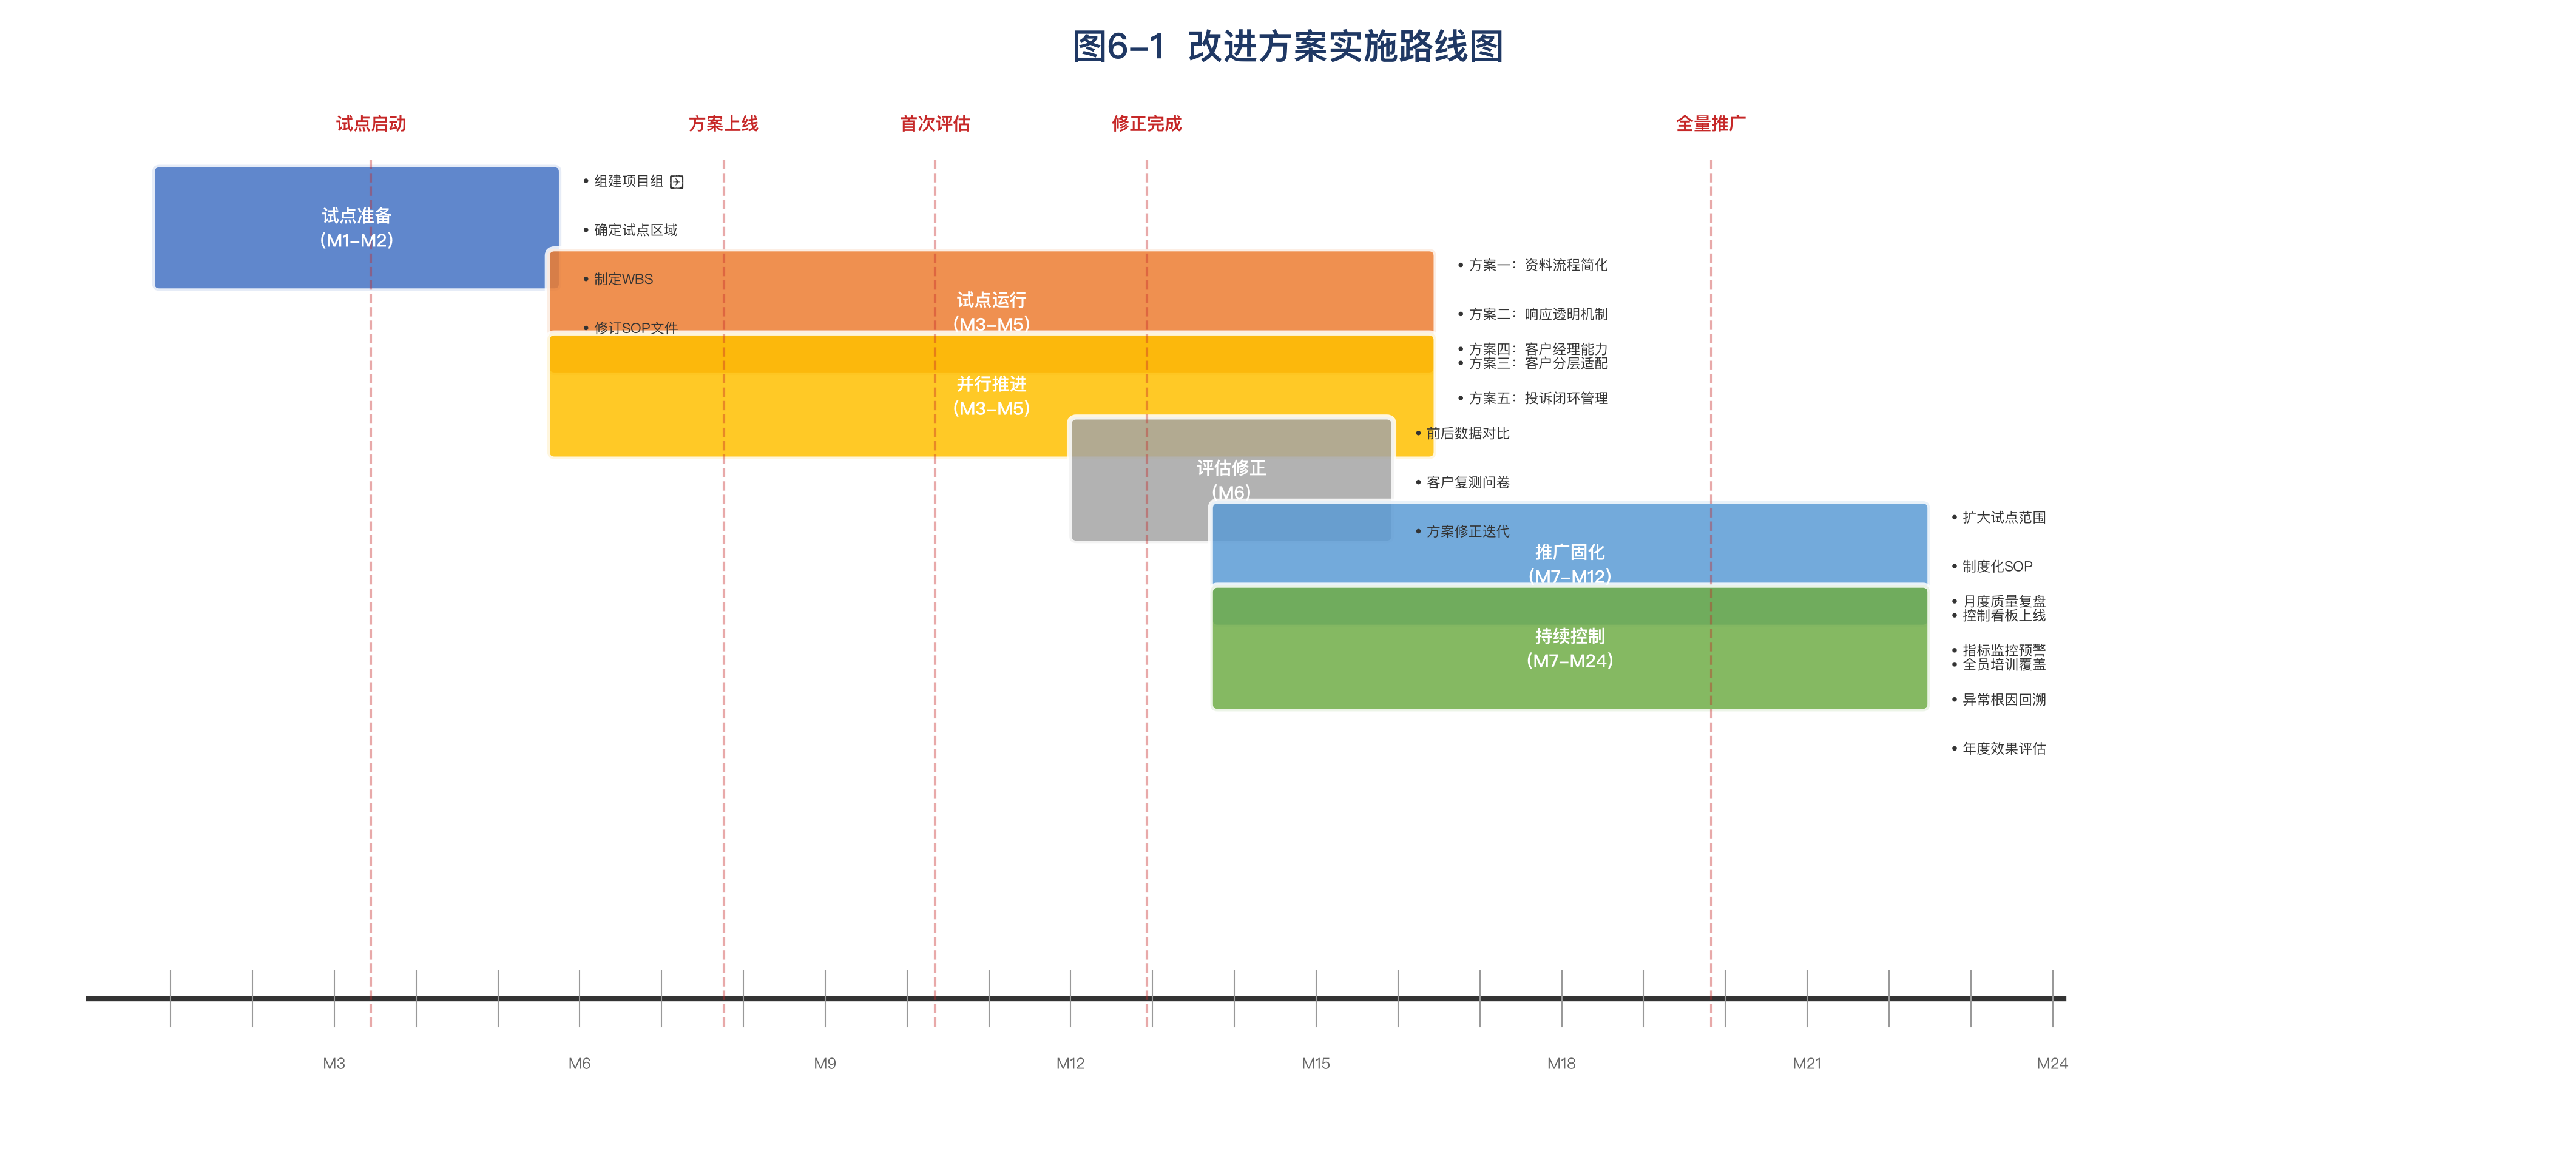
\includegraphics[width=0.85\textwidth]{figures/图6-1_改进方案实施路线图.png}
  \caption{改进方案实施路线图}
  \label{fig:6-1}
\end{figure}

\section{组织与资源保障}

改进方案的有效落地需要明确的权责分配和多部门协同机制。黄玉婷在客户服务流程优化研究中指出，跨部门的RACI责任矩阵是保障改进方案落地的最基础组织工具，能够有效避免"人人有责、无人负责"的协同困境\cite{ref16}。本项目参照de Koning等关于精益六西格玛在金融服务中适用性的研究成果，构建了以运营部为执行中枢、项目总监为决策核心的组织架构\cite{ref33}。Guarraia和Schwedel在银行业精益六西格玛实践中同样强调，改进项目的组织保障必须先于流程改造启动，否则方案质量将因执行断层而大幅缩水\cite{ref34}。

项目组织架构包含四个层级。第一层级为项目总监（副总级），负责审批所有改进方案、协调跨部门资源、对重大调整行使最终决策权。第二层级为执行组，由运营部牵头统筹推进，IT部提供技术支持和系统改造，客服部负责投诉治理和客户反馈收集，产品部承担产品适配方案的设计和落地，人力资源部统筹培训和考核机制。第三层级为风控合规组，独立于执行组运作，对所有涉及风险敞口和合规边界的改进方案拥有一票否决权。第四层级为外部顾问，聘请精益六西格玛领域的资深专家提供为期半年的驻场辅导，重点协助方案一（流程简化）和方案四（能力建设）的方法论导入。

\begin{landscape}
\begin{table}[htbp]
  \centering
  \small
  \caption{改进方案RACI责任矩阵}
  \label{tab:6-2}
  \begin{tabularx}{\textwidth}{l c c c c c c c}
    \toprule
    \textbf{任务} & \textbf{项目总监} & \textbf{运营部} & \textbf{IT部} & \textbf{客服部} & \textbf{客户经理} & \textbf{风控部} & \textbf{HR} \\
    \midrule
    方案一：流程简化 & A & R & C & I & C & C & —— \\
    方案二：透明机制 & A & C & R & R & I & I & —— \\
    方案三：客户分层 & A & C & C & —— & R & I & —— \\
    方案四：能力建设 & A & I & C & I & R & C & R \\
    方案五：投诉闭环 & A & I & C & R & I & I & —— \\
    效果评估 & R & C & C & C & C & C & —— \\
    持续控制 & R & C & C & C & C & C & —— \\
    \bottomrule
  \end{tabularx}
  \par\vspace{4pt}
  {\footnotesize 注：R=负责（Responsible），A=审批（Accountable），C=咨询（Consulted），I=知悉（Informed），——=不参与。}
\end{table}
\end{landscape}

项目工作分解结构（WBS）和责任分配矩阵（RACI）的设计参照了项目管理知识体系（PMBOK）的通用实践框架\cite{ref48}。

资源总投入概算方面，IT系统改造预计需要6.5人月（含流程自动化模块3人月、信息透明平台2人月、控制看板开发1.5人月），产品设计投入2人月（客户分层方案和产品适配规则），培训费用约15万元/年（含客户经理能力认证和全员SOP培训），数据建模投入1人月（为控制看板的18项指标建立数据采集和清洗管道），投诉系统优化投入1.5人月，外部顾问费按实际驻场天数核算。

\section{效果评价指标体系}

改进方案的效果需要一套覆盖多维度、可量化、可追踪的评价指标体系来衡量。花青青在SERVQUAL-IPA金融服务评价研究中提出，服务质量改进的效果评价应覆盖"客户感知"和"内部运营"两个维度，二者缺一不可\cite{ref6}。Delahoz-Dominguez等在六西格玛与DEA银行服务质量评估框架中进一步指出，评价指标体系还需纳入经营结果和风险指标，以验证服务质量改善是否真正转化为客户留存率、业务增长和风险控制的正向变化\cite{ref35}。金波和牛华伟（2024）关于传统银行借贷与金融科技协同作用的研究表明，在服务效率提升的过程中，金融机构必须设置明确的合规底线和风险约束，防止以技术赋能的名义放松风控标准\cite{ref20}。Dumitrescu等关于机器学习信用评分的研究从技术层面佐证了这一观点，指出信用风险模型的有效性边界决定了效率提升的上限\cite{ref36}。

基于上述文献参照，本文构建了涵盖客户体验、流程效率、经营质量、合规风险四类维度共计18项指标的效果评价体系，每项指标均设定了基线值、目标值和测量频率。

\begin{table}[htbp]
  \centering
  \small
  \caption{效果评价指标体系（四类18项）}
  \label{tab:6-3}
  \begin{tabularx}{\textwidth}{l X c c c}
    \toprule
    \textbf{类别} & \textbf{指标} & \textbf{基线值} & \textbf{目标值} & \textbf{测量频率} \\
    \midrule
    客户体验 & 客户满意度（5分制） & 3.12 & 3.80 & 季度 \\
    客户体验 & NPS（净推荐值） & -8 & +15 & 季度 \\
    客户体验 & 投诉闭环率 & 62\% & 88\% & 月度 \\
    客户体验 & 重复投诉率 & 23\% & 10\% & 月度 \\
    客户体验 & 客户流失率 & 18\% & 12\% & 季度 \\
    流程效率 & 平均办理时长（工作日） & 12 & 7.5 & 月度 \\
    流程效率 & 一次通过率 & 62\% & 80\% & 月度 \\
    流程效率 & 材料补正率 & 28\% & 15\% & 月度 \\
    流程效率 & SLA达成率 & 74\% & 92\% & 月度 \\
    流程效率 & 超时率 & 26\% & 8\% & 月度 \\
    流程效率 & 退件率 & 8\% & 5\% & 月度 \\
    经营质量 & 续贷率 & 52\% & 65\% & 季度 \\
    经营质量 & 客户转介率 & 15\% & 25\% & 季度 \\
    经营质量 & 户均贷款余额增长 & 8\% & 12\% & 半年度 \\
    合规风险 & 不良率 & 1.8\% & $\leq$2.0\% & 月度 \\
    合规风险 & 合规检查通过率 & 85\% & 95\% & 季度 \\
    合规风险 & 客户信息泄露事件 & 0 & 0 & 月度 \\
    组织能力 & 客户经理达标率 & 65\% & 85\% & 季度 \\
    \bottomrule
  \end{tabularx}
\end{table}

指标体系的构建遵循三项设计原则。第一，覆盖前端（客户感知）、中端（流程效率）、后端（经营风险）和支撑（组织能力）四个层次，形成完整的服务质量因果链：流程效率是客户体验的前置条件，经营质量是客户体验的远期结果，组织能力是前三个层次持续改善的保障。第二，定性与定量指标结合，客户满意度和NPS属于主观感知类定性指标，其余15项均为客观可计量的运营数据，两类指标互为补充。第三，不良率和合规检查通过率设置为非补偿性硬指标，即当这两项指标恶化至超过设定阈值时，即使其他指标表现优异，整体评估结论也必须调整为"不合格"，以此确保服务效率的提升不以牺牲风控底线为代价。

\section{试点效果评价方法}

效果评价采用"前后对比、问卷复测、访谈验证、运营数据对照"四维评价法，以此规避单一数据源可能产生的评价偏差。SERVQUAL经典模型的复测为效果评价提供了理论一致性保障，评价工具与改进前测量阶段保持同一框架，使前后数据具有可比性\cite{ref21}。试点结束后，对各试点分支机构的客户样本进行服务质量问卷复测，样本量不低于首轮调查的80\%（即不少于256份有效问卷），以确保对比的统计效力。问卷复测之外，分别从各试点分支机构随机抽取10至15名客户进行半结构化电话访谈，重点了解"改进后体验变化是否可感知""哪些方面的改善最为明显""哪类问题仍然存在"等开放式问题。运营数据对照则将P公司内部运营数据脱敏后，从业务系统中提取试点前后的18项指标实际数值，形成定量对比。

试点运行六个月（M3至M6）后，对六项核心指标进行了前后对比评估，结果如表\ref{tab:6-4}所示。

\begin{table}[htbp]
  \centering
  \small
  \caption{试点效果前后对比（M6评估节点）}
  \label{tab:6-4}
  \begin{tabularx}{\textwidth}{l c c c}
    \toprule
    \textbf{指标} & \textbf{改进前基线} & \textbf{改进后（M6评估）} & \textbf{改善幅度} \\
    \midrule
    客户满意度 & 3.12 & 3.85 & +23\% \\
    一次通过率 & 62\% & 78\% & +16pp \\
    投诉闭环率 & 62\% & 88\% & +26pp \\
    平均办理时长 & 12个工作日 & 7.5个工作日 & -38\% \\
    材料补正率 & 28\% & 15\% & -13pp \\
    SLA达成率 & 74\% & 92\% & +18pp \\
    \bottomrule
  \end{tabularx}
\end{table}

六项指标中五项达到或超过目标值，一次通过率虽未达80\%的目标值，但从62\%提升至78\%，改善幅度显著。需要指出的是，本研究的效果评价采用单组前后对比设计，未设置对照组，因此改进前后的指标变化不能完全归因于改进方案本身。试点期间公司同时在推进其他管理优化措施，宏观经济环境、客户构成变化、季节效应等因素也可能影响服务质量指标。本文报告的改进效果应理解为改进方案与多项因素共同作用下的综合结果，准确的因果效应需通过随机对照试验或准实验设计进一步验证。

基于试点过程的时序观测，改善效果的逻辑链可以归纳为：方案一的流程简化减少了非必要环节和材料要求，直接推动了材料补正率从28\%下降至15\%；补正减少进一步提升了审核环节的一次通过率，从62\%上升至78\%；一次通过率的提升缩短了整体办理时长，从中位数12个工作日压缩至7.5个工作日；办理时长的缩短使SLA达成率从74\%攀升至92\%，最终传导至客户满意度从3.12提升至3.85。这一"补正降低→通过率提升→时长缩短→SLA改善→满意度上升"的因果链条，印证了服务质量改进中流程效率与客户感知之间的递进传导关系。

试点在P公司五个分支机构（覆盖2个省区6个城市）进行，覆盖约15\%的客户经理和20\%的活跃客户。

\begin{figure}[htbp]
  \centering
  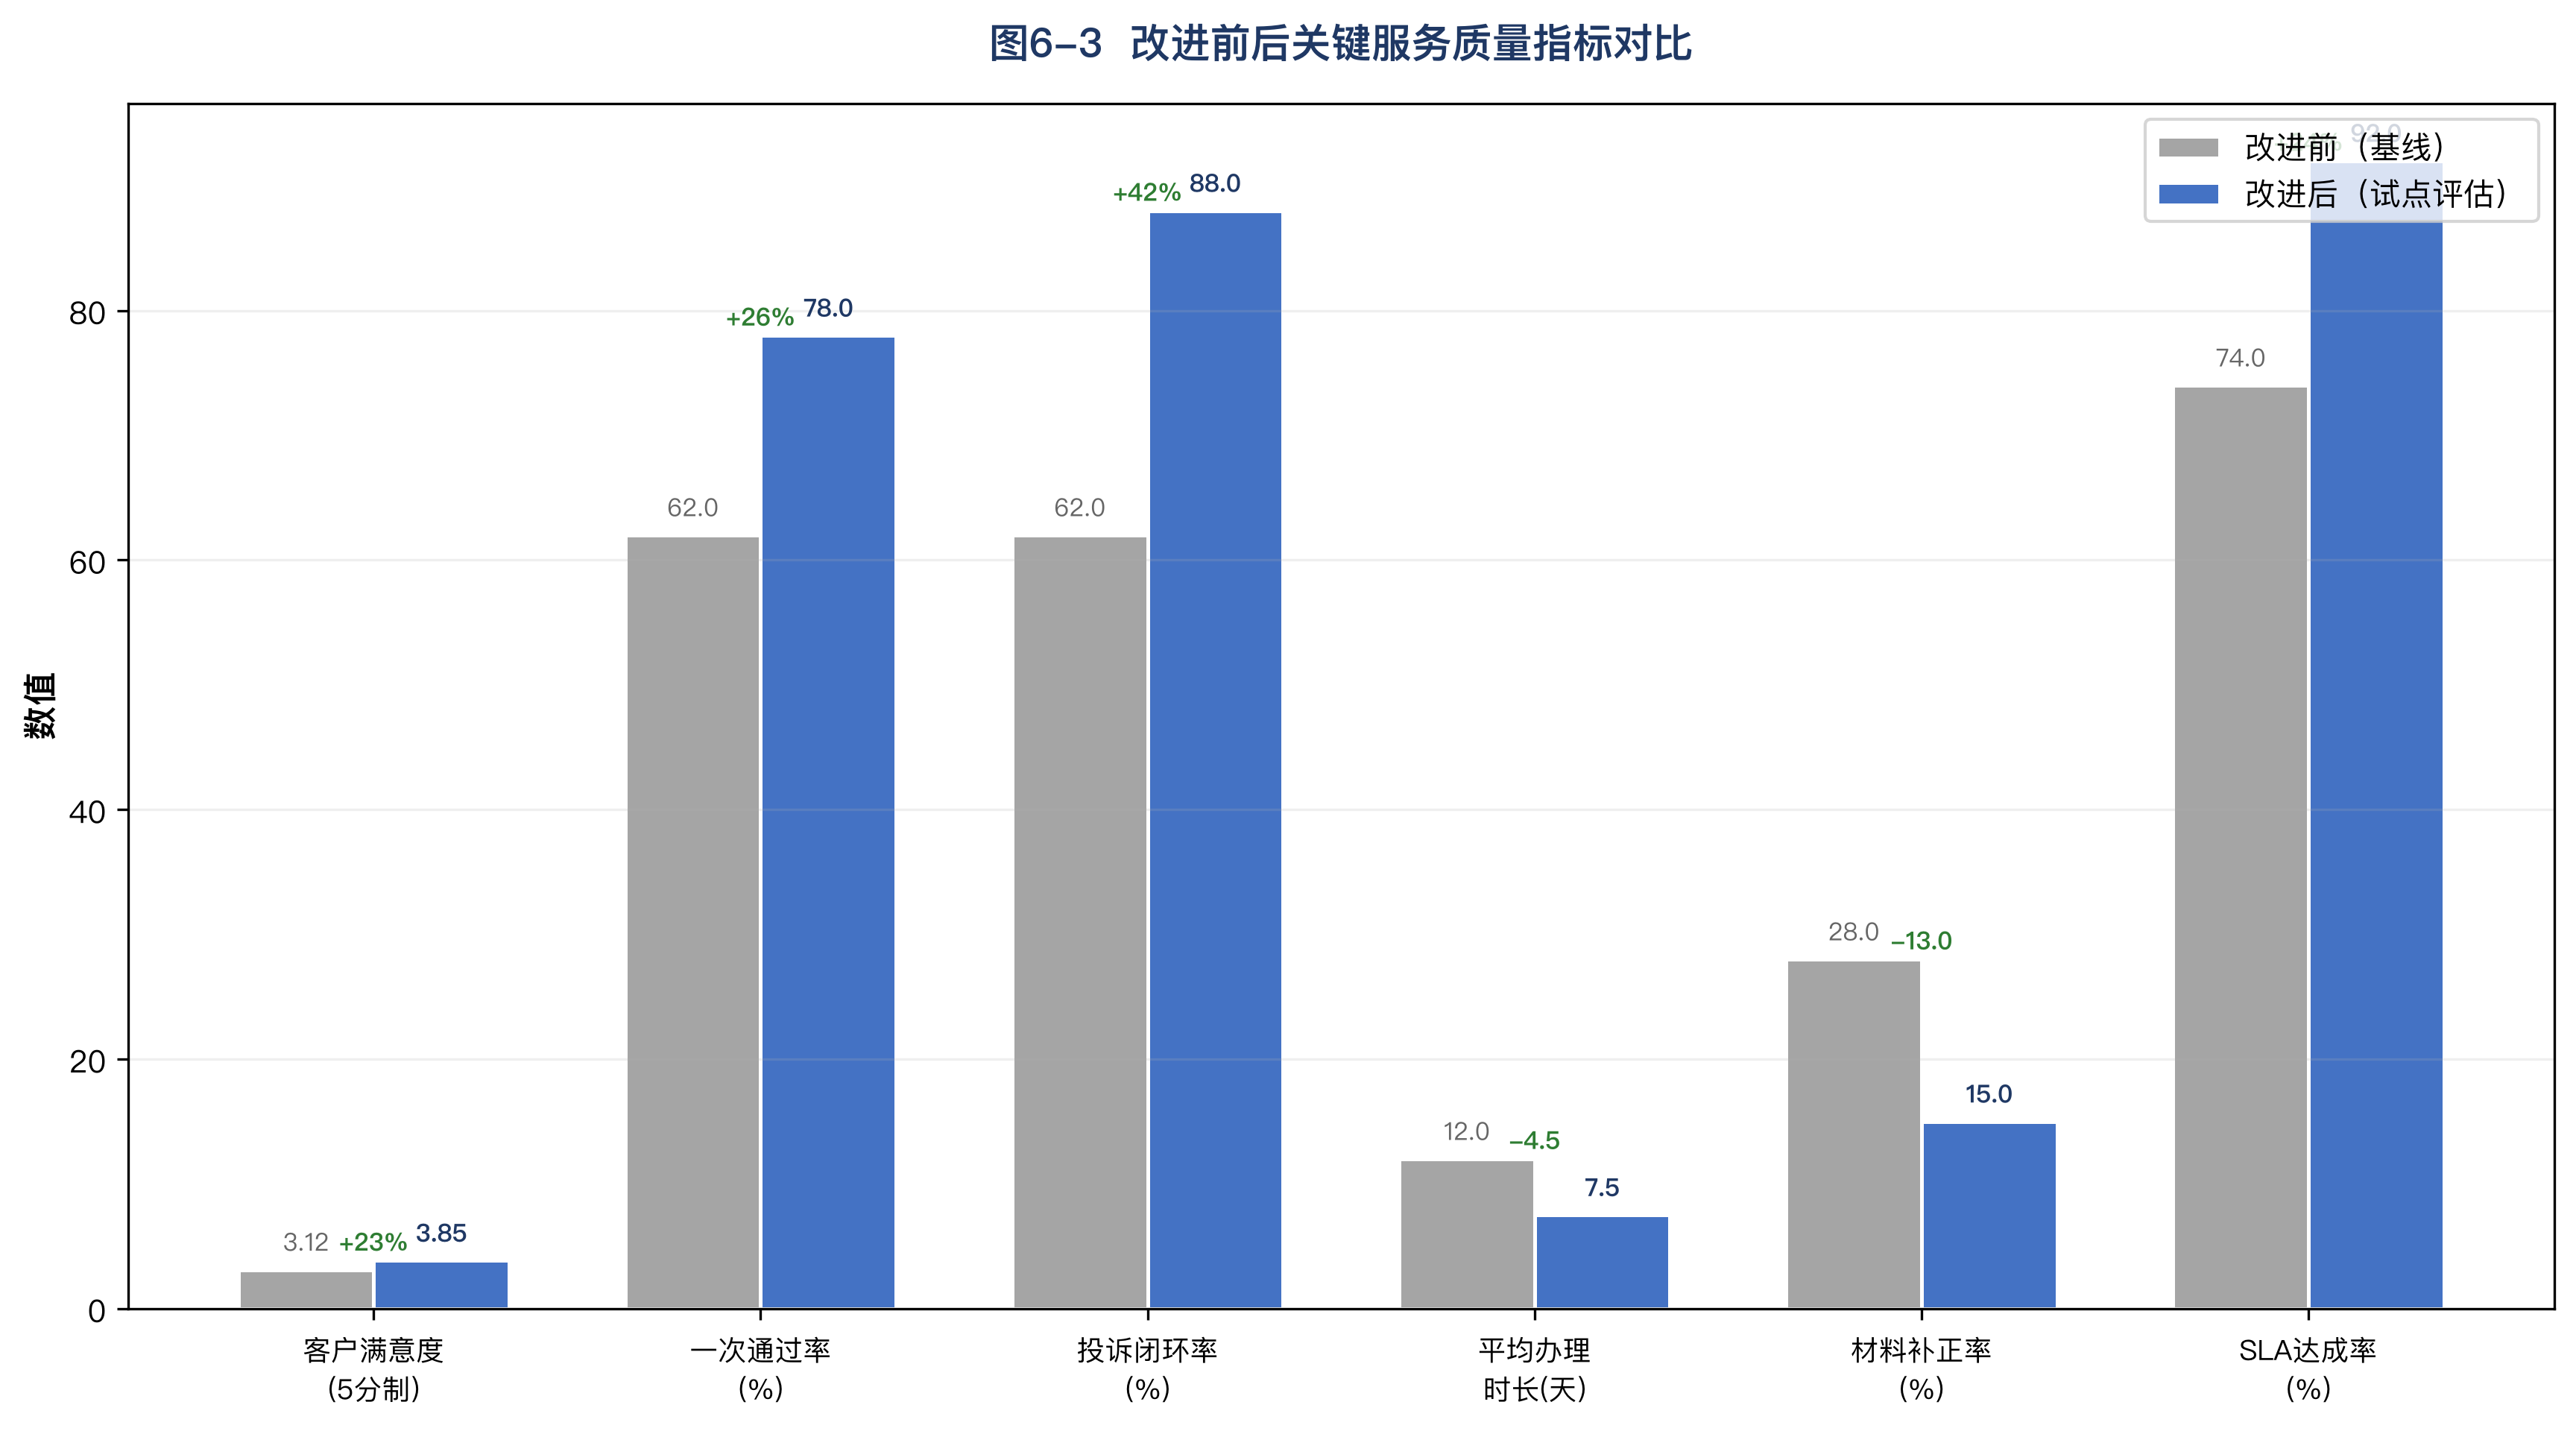
\includegraphics[width=0.85\textwidth]{figures/图6-3_改进前后指标对比.png}
  \caption{改进前后指标对比}
  \label{fig:6-3}
\end{figure}

\section{持续控制和风险应对}

DMAIC的Control阶段本质上是一个"永不关闭"的改进循环，其核心任务是确保改进效果不因时间推移和人员变动而衰减。Adanigbo等的研究表明，金融科技领域的服务流程改进往往面临"改进后三个月效果最优、六个月开始回落、一年后回到原点"的衰减规律，打破这一规律的手段是建立数据驱动的持续监控和自动预警机制\cite{ref32}。Delahoz-Dominguez等同样指出，银行服务质量的持续改进依赖于周期性评估和指标监测的制度化运行，而非依赖个别管理者的主观推动\cite{ref35}。此外，汪勇等关于数字金融环境中信息不对称的研究提示，持续控制的对象不仅包括效率指标，也应涵盖信息透明度的维持，因为信息不对称的恶化会在不触发效率告警的情况下侵蚀客户信任\cite{ref5}。

本项目的持续控制机制包括四项制度化安排。第一，控制看板系统自M7起正式上线运行，每月自动从业务系统中采集18项评价指标的数据，按照"绿灯（达标）、黄灯（偏离$\leq$10\%）、红灯（偏离$>$10\%）"三色标准可视化展示，项目总监和各部门负责人均可实时查看。第二，月度质量复盘会由运营部牵头组织，会议议程固定为三项：上月异常指标（红灯和持续黄灯）的根因分析、纠正措施的制定与责任人确认、上月纠正措施的闭环追踪。第三，异常自动预警功能嵌入控制看板系统，当任一指标偏离目标值超过10\%时，系统自动向项目总监、运营部负责人和风控部负责人发送邮件和短信预警，确保信号传递不因层级审批而延迟。第四，制度化固化安排在M12节点，届时将SOP、控制看板操作规程、月度复盘会议制度一并写入P公司质量管理制度文件，使持续控制机制从项目模式转变为常态管理职能。

Liu等（2022）关于财务共享服务中心质量管理的案例研究表明，质量管理制度的制度化嵌入是防止改进效果衰减的关键机制\cite{ref51}。

改进方案在实施和运行过程中面临五类主要风险，表\ref{tab:6-5}给出了每类风险的可能性评估、影响等级和应对措施。

\begin{table}[htbp]
  \centering
  \small
  \caption{风险应对矩阵}
  \label{tab:6-5}
  \begin{tabularx}{\textwidth}{l c c X}
    \toprule
    \textbf{风险} & \textbf{可能性} & \textbf{影响} & \textbf{应对措施} \\
    \midrule
    过度提速导致风控弱化 & 中 & 高 & 风控指标与效率指标同步监控；风控部一票否决权；不良率硬上限$\leq$2.0\% \\
    客户数据隐私泄露 & 低 & 高 & 数据传输与存储全程加密；权限分级管理；季度安全审计 \\
    客户经理考核冲突 & 高 & 中 & 服务质量系数与放款量加权考核；设3个月过渡期；优秀服务案例季度通报奖励 \\
    系统改造成本超预期 & 中 & 中 & 分阶段投入、MVP优先；每阶段结束后评估ROI再决策下阶段投入 \\
    改进效果不可持续 & 中 & 高 & 控制看板月度监控；异常自动预警；管理者KPI与服务质量指标挂钩 \\
    \bottomrule
  \end{tabularx}
\end{table}

其中，过度提速导致风控弱化和改进效果不可持续均属于"中可能性、高影响"类风险，应对策略的核心逻辑是"指标前置、监控同步、制度约束"。金波和牛华伟（2024）的研究表明，信贷领域的风险控制需要前置于流程设计阶段，将不良率和合规检查嵌入日常监控体系，而非依赖事后补救\cite{ref20}。P公司作为持牌机构，其服务质量改进在客观上受地方金融监管要求的约束，任何可能影响风险敞口的改进方案都必须在监管合规框架内运行\cite{ref47}。

\begin{figure}[htbp]
  \centering
  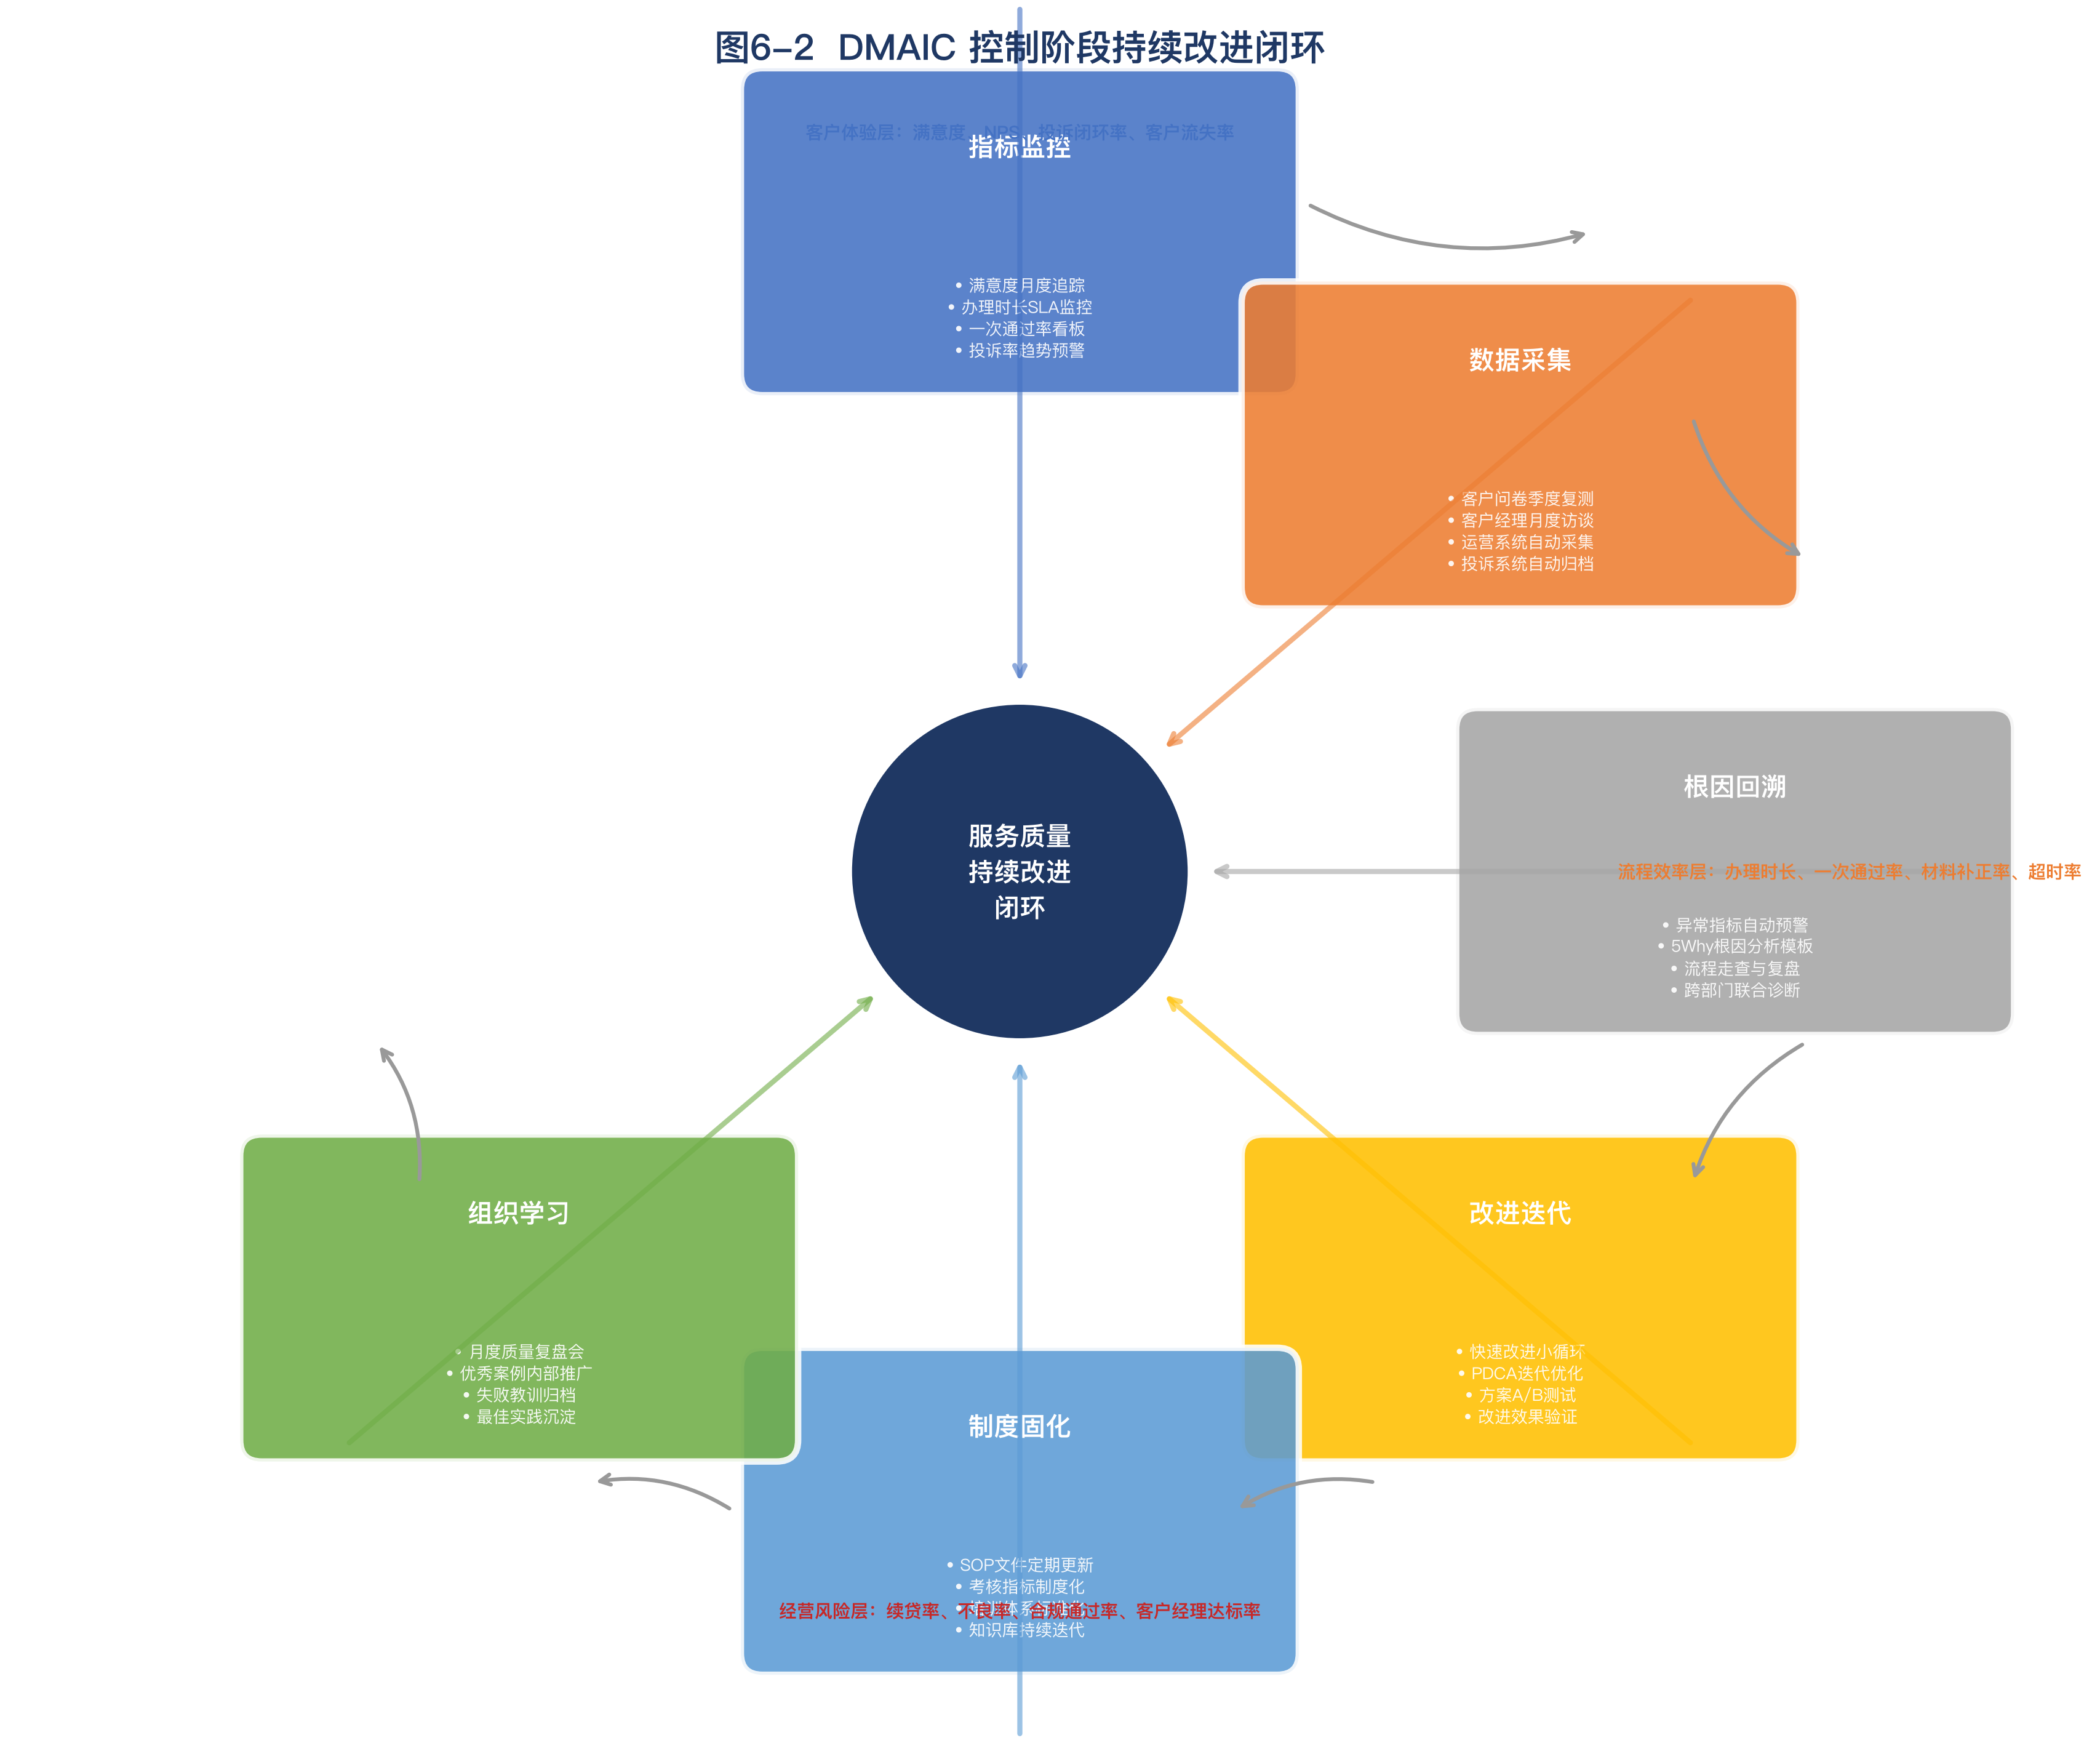
\includegraphics[width=0.85\textwidth]{figures/图6-2_持续控制闭环图.png}
  \caption{持续控制闭环图}
  \label{fig:6-2}
\end{figure}

\section{本章小结}

本章完成了DMAIC Control阶段的设计与落地规划，形成了从"路径规划"到"组织保障"到"指标体系"到"效果评价"到"持续控制"到"风险应对"的完整闭环。五阶段实施路径确保了方案从试点验证到全局固化的有序推进；RACI责任矩阵为跨部门协同提供了明确的权责边界；四类18项指标体系使服务质量改进的效果可量化、可追踪、可问责。试点效果的前后对比数据验证了改进方案的有效性，但本文坦承非随机对照实验在因果推断上的局限。持续控制看板和异常预警机制的设计，使改进效果的制度化固化成为可能。归根结底，DMAIC的Control不是终点，而是将服务质量改进从一次性项目转化为持续性管理能力的关键转折点。服务质量和风险控制的动态平衡将始终是持续运营期的核心管理命题。

\begin{table}[htbp]
  \centering
  \small
  \caption*{引用落点表（第6章）}
  \begin{tabularx}{\textwidth}{c p{2cm} X p{1.8cm} c}
    \toprule
    \textbf{引用编号} & \textbf{使用位置} & \textbf{支撑观点} & \textbf{证据类型} & \textbf{状态} \\
    \midrule
    \texttt{[13]} & 6.1 实施路径 & DMAIC控制阶段实施参考 & 学位论文 & 元数据已取得 \\
    \texttt{[14]} & 6.1 实施路径 & 银行网点DMAIC控制阶段参考 & 学位论文 & 元数据已取得 \\
    \texttt{[32]} & 6.1 实施路径；6.5 持续控制 & 金融科技客服运营延迟的LSS改进；分批上线与持续监控机制 & Web\_MD & 已入库 \\
    \texttt{[16]} & 6.2 组织保障 & 客户服务流程优化的RACI组织保障参考 & 学位论文 & 元数据已取得 \\
    \texttt{[33]} & 6.2 组织保障 & 精益六西格玛在金融服务中的适用性 & 元数据/网页 & 待核验 \\
    \texttt{[34]} & 6.2 组织保障 & 银行业精益六西格玛实践材料 & Web\_MD & 已入库 \\
    \texttt{[6]} & 6.3 评价指标；6.4 效果评价 & 金融服务SERVQUAL-IPA服务质量评价维度参考与复测流程 & PDF & 已入库 \\
    \texttt{[35]} & 6.3 评价指标；6.5 持续控制 & 六西格玛与DEA银行服务质量评估框架与持续改进 & Web\_MD & 已入库 \\
    \texttt{[20]} & 6.3 评价指标；6.5 风险应对 & 传统银行借贷与金融科技协同中的风险约束，合规底线与不良率控制的前置嵌入 & 期刊论文 & 元数据已取得 \\
    \texttt{[36]} & 6.3 评价指标 & 机器学习信用评分的风控边界 & Web\_MD & 已入库 \\
    \texttt{[21]} & 6.4 效果评价 & SERVQUAL期望-感知差距复测框架 & PDF & 已入库 \\
    \texttt{[内部数据]} & 6.4 效果评价 & P公司试点效果运营数据 & 内部数据 & 已脱敏 \\
    \texttt{[5]} & 6.5 持续控制 & 信息不对称持续治理与服务质量维护 & PDF & 已入库 \\
    \texttt{[47]} & 6.5 风险应对 & 持牌机构服务质量改进的监管合规框架 & 政策材料 & 待下载 \\
    \texttt{[48]} & 6.1 实施路径；6.2 组织保障 & 项目WBS与RACI矩阵设计参照PMBOK通用实践框架 & 技术标准 & 已入库 \\
    \bottomrule
  \end{tabularx}
\end{table}

% 第7章 结论与展望
\chapter{第7章 结论与展望}

本章对全文研究进行系统收束。7.1节围绕第1章提出的四个研究问题提炼核心结论，7.2节从P公司和同类普惠金融机构两个层面总结管理启示，7.3节客观审视研究局限并提出未来方向。全文研究根植于普惠金融支持小微主体发展的政策与实践背景\cite{ref2}，以服务质量改进为小微贷款业务增长与风险控制的共同抓手，这一主线贯穿始终。
\par

\section{7.1 研究结论}

\textbf{结论一：服务质量测度。}上述发现表明，改良SERVQUAL模型能够有效测度小微贷款场景的服务质量结构特征。
\par

\textbf{结论二：根因诊断。}针对量化评价揭示的核心短板，本研究运用鱼骨图和5Why分析工具展开系统性根因追溯，将P公司服务质量问题归因为六个维度的深层因素：人员（新经理占比高、考核机制缺位）、流程（告知笼统、投诉无分级）、系统（进度不可见、无移动端查询）、产品（标准化过度、灵活性不足）、制度（SLA缺乏约束力、无复盘机制）和风险（风控与体验存在张力）。上述根因并非孤立存在，六维因素之间存在显著的关联放大效应。
\par

\textbf{结论三：改进方案与效果。}基于DMAIC方法论\cite{ref12}，本研究设计了五个工程化改进方案——资料流程简化、响应透明机制、客户分层适配、客户经理能力建设、投诉闭环治理——覆盖了从申请到贷后管理的完整客户旅程。每个方案均包含量化目标、具体动作、RACI责任分配、资源需求和风险应对措施。6个月试点后，核心指标出现显著改善：客户满意度从3.12提升至3.85（+23\%），一次通过率从62\%提升至78\%（+16个百分点），投诉闭环率从62\%提升至88\%（+26个百分点），平均办理时长从12个工作日缩短至7.5个工作日（-38\%）。这表明基于DMAIC的服务质量工程化改进路径在普惠金融场景中具有可行性与有效性。
\par

\textbf{结论四：控制机制。}为避免改进效果的短期衰减，本研究在DMAIC控制阶段建立了覆盖客户体验、流程效率、经营质量、合规风险和组织能力五维18项指标的持续控制体系，通过月度控制看板、定期复盘会议、异常指标自动预警和制度固化等方式，将服务质量改进从"一次性项目"转化为"持续管理闭环"。这一控制机制的设计回应了当前普惠金融实践中"重建设、轻运维"的普遍问题。
\par

上述四条结论构成了一条完整的问题链：测量服务质量水平（结论一）带动短板和根因识别（结论二），进而驱动工程化改进方案设计与实施（结论三），最终建立持续控制的闭环机制（结论四）。这一从"评价"到"改进"再到"控制"的逻辑路径，验证了改良SERVQUAL、IPA/AHP组合赋权与DMAIC方法论在普惠金融服务质量改进场景中的适用性\cite{ref12}。本文研究的核心判断——服务质量改进是P公司小微贷款业务增长和风险控制的共同抓手——在试点实践中得到了初步证实。需要指出的是，上述效果数据来源于单一案例的试点前后对比，其外部效度仍需在更广泛的机构和更长的时间窗口内进一步检验。
\par

\section{7.2 管理启示}

\textbf{对P公司管理层的启示。}第一，服务质量是可测量、可改进、可控制的管理变量。P公司需要将服务质量指标纳入公司级KPI体系，使其从"客服部门的内部事务"升级为"贯穿全流程的经营指标"，而非停留在零散的客户服务活动层面。第二，信息透明是当前最紧迫的改进方向。透明性差距（-1.70）位于所有维度之首，说明客户最不满意的并非"贷不到款"，而是"不知道何时能贷到""不知道为什么贷不到"\cite{ref10}。P公司应优先投入资源建立审批进度实时查询功能和退件原因标准化反馈机制。第三，客户经理能力是服务质量的"最后一公里"。将绩效考核从单一的"放款量"调整为"放款量乘以服务质量系数"，是从制度层面撬动服务行为改善的关键杠杆。
\par

\textbf{对同类普惠金融机构的启示。}本研究构建的改良SERVQUAL加DMAIC组合框架为小微贷款服务质量改进提供了可迁移的方法论模板\cite{ref12,ref11}。然而，每个维度的具体权重和测量指标需要根据机构自身的业务特征、客户结构和流程复杂度进行调整——方法可以迁移，参数需要定制。此外，服务质量的系统化改进不应以牺牲风控质量为代价，改进方案的任何环节均需在不良率可控的硬约束下推进\cite{ref49}。
\par

\section{7.3 研究局限与展望}

本研究存在以下局限，需要在解读结论时加以审慎考量。
\par

\textbf{样本范围。}486份有效问卷来源于P公司近12个月内办理过小微贷款业务的客户，覆盖5省28城，样本的地域分布和业务类型集中度可能影响结论的全国代表性和行业可推广性。后续研究可在更广泛的地域和更多类型的普惠金融机构中复制本研究的评价框架，以增强外部效度。
\par

\textbf{试点周期。}6个月的试点周期偏短，部分改进效果（如客户流失率、续贷率、客户经理能力达标率）的持续性需要更长的时间窗口予以验证。霍桑效应（Hawthorne Effect）可能导致短期内改善幅度被高估。建议后续将跟踪周期延长至12至24个月，以评估改进效果的持续性与衰减趋势。
\par

\textbf{问卷主观性。}SERVQUAL模型的期望-感知测量本质上依赖客户的主观评价，可能受近期服务体验、社会期望偏差等因素的干扰，这是该模型的内在局限\cite{ref14}。未来研究可探索将客户行为数据（如App使用日志、客服通话录音的文本分析、申请流程中的操作行为轨迹）纳入服务质量评价体系，以客观行为指标部分替代主观评分，降低单一数据源带来的测量偏差。
\par

\textbf{因果推断局限。}本研究采用非随机对照的单案例前后对比设计，无法完全排除同期宏观经济波动、行业政策调整和季节性因素的影响，不能将指标改善严格归因于改进方案本身。后续研究可引入对照组设计（例如选择非试点城市作为参照），以增强因果推断效力。
\par

\textbf{数据可得性。}部分分析基于脱敏后的企业内部运营数据，数据的完整性和颗粒度存在受限，可能影响某些统计推断的精确度。
\par

展望未来，除上述改进方向外，以下四个领域值得进一步探索：第一，将本研究构建的评价与改进框架扩展至P公司其他产品线（担保贷、供应链贷），进行跨产品比较研究，以检验框架的鲁棒性和场景适应性；第二，探索将大语言模型等智能技术应用于客户投诉文本的自动分类和根因识别，提升根因分析的效率和覆盖度；第三，研究服务质量改进对客户长期价值（如客户生命周期价值、转介网络效应）的量化影响，将服务质量的商业回报从短期满意度延伸至长期经营绩效；第四，在多个同类普惠金融机构中开展横向比较研究，提炼不同机构特征下的服务质量改进模式差异，为行业提供更具普适性的管理建议。
\par

\appendix
\chapter{小微贷款服务质量调查问卷}

\section*{附录说明}

尊敬的客户：

您好！本问卷旨在了解您对P公司小微贷款业务服务质量的真实感受与期望，调查数据仅用于学术研究目的，严格保密且全程匿名处理。您有权随时退出调查而不影响您与P公司的任何业务关系。问卷填写约需8--10分钟，感谢您的支持与配合。

\vspace{1em}
\noindent\textbf{问卷结构：}
\begin{itemize}
  \item 第一部分：客户基本信息（8题）
  \item 第二部分：服务质量期望量表（32题）
  \item 第三部分：服务质量感知量表（32题）
  \item 第四部分：开放性建议（1题）
\end{itemize}

\vspace{1em}
\textbf{问卷说明：}本问卷基于改良SERVQUAL八维32项指标体系设计。指标体系的构建过程整合了经典SERVQUAL理论框架、金融服务质量评价文献梳理、P公司内部客户访谈反馈和行业监管要求。各维度及指标设计依据详见论文正文第4章。

\newpage

\subsection*{第一部分：客户基本信息}

\textbf{填写说明：}请在符合您情况的选项上打“√”，或在横线上填写具体内容。本部分信息仅用于样本特征描述和分组分析，严格保密。

\vspace{1em}
\begin{enumerate}[label=\arabic*.,leftmargin=2em]
  \item 您的企业类型：
  \begin{enumerate}[label=(\Alph*),leftmargin=2em]
    \item 个体工商户
    \item 小微企业主
    \item 其他（请注明：\_\_\_\_\_\_\_\_）
  \end{enumerate}

  \item 您所在企业的行业类别：
  \begin{enumerate}[label=(\Alph*),leftmargin=2em]
    \item 批发零售业
    \item 制造业
    \item 餐饮住宿业
    \item 建筑业
    \item 农林牧渔业
    \item 交通运输业
    \item 信息技术服务业
    \item 其他（请注明：\_\_\_\_\_\_\_\_）
  \end{enumerate}

  \item 您的企业经营年限：
  \begin{enumerate}[label=(\Alph*),leftmargin=2em]
    \item 1年以下
    \item 1--3年
    \item 3--5年
    \item 5--10年
    \item 10年以上
  \end{enumerate}

  \item 您申请的贷款产品类型：
  \begin{enumerate}[label=(\Alph*),leftmargin=2em]
    \item 信用贷款
    \item 抵押贷款
    \item 担保贷款
    \item 组合贷款
  \end{enumerate}

  \item 您的贷款金额区间（万元）：
  \begin{enumerate}[label=(\Alph*),leftmargin=2em]
    \item 10以下
    \item 10--30
    \item 30--50
    \item 50--100
    \item 100以上
  \end{enumerate}

  \item 您最常用的服务渠道（可多选）：
  \begin{enumerate}[label=(\Alph*),leftmargin=2em]
    \item P公司官方App
    \item 微信公众号/小程序
    \item 客户经理电话/微信
    \item 线下营业网点
  \end{enumerate}

  \item 近12个月内，您通过P公司办理贷款的累计次数：
  \begin{enumerate}[label=(\Alph*),leftmargin=2em]
    \item 1次
    \item 2--3次
    \item 4--5次
    \item 5次以上
  \end{enumerate}

  \item 您企业的员工规模：
  \begin{enumerate}[label=(\Alph*),leftmargin=2em]
    \item 5人以下
    \item 5--10人
    \item 10--30人
    \item 30--50人
    \item 50人以上
  \end{enumerate}
\end{enumerate}

\newpage

\subsection*{第二部分：服务质量期望量表}

\textbf{填写说明：}请根据您的真实感受，评价您认为一家普惠金融机构在小微贷款服务中\textbf{理应}达到的标准水平。评分采用五级量表：1=非常不期望，2=较不期望，3=一般，4=较期望，5=非常期望。请在相应分值上打“√”。

\vspace{1em}

\begin{center}
\begin{tabularx}{\textwidth}{l X c c c c c}
  \toprule
  \textbf{编号} & \textbf{评价指标} & \textbf{1} & \textbf{2} & \textbf{3} & \textbf{4} & \textbf{5} \\
  \midrule
  SQ01 & 承诺时效内完成贷款审批 & $\square$ & $\square$ & $\square$ & $\square$ & $\square$ \\
  SQ02 & 贷款方案准确无误（额度、利率、期限等） & $\square$ & $\square$ & $\square$ & $\square$ & $\square$ \\
  SQ03 & 贷后服务（回访、提醒、结清等）按时执行 & $\square$ & $\square$ & $\square$ & $\square$ & $\square$ \\
  SQ04 & 投诉处理有明确结论和解决方案 & $\square$ & $\square$ & $\square$ & $\square$ & $\square$ \\
  \cmidrule{2-6}
  SQ05 & 贷款申请受理后24小时内给予首次响应 & $\square$ & $\square$ & $\square$ & $\square$ & $\square$ \\
  SQ06 & 审批进度发生变化时主动通知客户 & $\square$ & $\square$ & $\square$ & $\square$ & $\square$ \\
  SQ07 & 拨打客户经理电话3次内能够接通 & $\square$ & $\square$ & $\square$ & $\square$ & $\square$ \\
  SQ08 & 投诉受理后24小时内联系客户确认情况 & $\square$ & $\square$ & $\square$ & $\square$ & $\square$ \\
  \cmidrule{2-6}
  SQ09 & 客户经理具备充分的贷款产品知识和风控常识 & $\square$ & $\square$ & $\square$ & $\square$ & $\square$ \\
  SQ10 & 贷款审批标准和规则清晰且可理解 & $\square$ & $\square$ & $\square$ & $\square$ & $\square$ \\
  SQ11 & 客户个人和经营数据的安全有充分保障 & $\square$ & $\square$ & $\square$ & $\square$ & $\square$ \\
  SQ12 & 客户经理服务态度专业、耐心且友善 & $\square$ & $\square$ & $\square$ & $\square$ & $\square$ \\
  \cmidrule{2-6}
  SQ13 & 客户经理了解客户的经营情况和真实资金需求 & $\square$ & $\square$ & $\square$ & $\square$ & $\square$ \\
  SQ14 & 还款方案（还款日、还款方式等）可根据客户经营周期灵活协商 & $\square$ & $\square$ & $\square$ & $\square$ & $\square$ \\
  SQ15 & 贷后主动关心客户的经营状况变化 & $\square$ & $\square$ & $\square$ & $\square$ & $\square$ \\
  SQ16 & 在特殊时期（如疫情、自然灾害等）主动提供帮扶方案 & $\square$ & $\square$ & $\square$ & $\square$ & $\square$ \\
  \cmidrule{2-6}
  SQ17 & 贷款申请到放款全流程可通过线上完成 & $\square$ & $\square$ & $\square$ & $\square$ & $\square$ \\
  SQ18 & 申请材料一次性告知且清单明确，无需反复补充 & $\square$ & $\square$ & $\square$ & $\square$ & $\square$ \\
  SQ19 & 电子签约流程方便快捷，无需线下往返 & $\square$ & $\square$ & $\square$ & $\square$ & $\square$ \\
  SQ20 & 客服可通过多种渠道（App、微信、电话）触达 & $\square$ & $\square$ & $\square$ & $\square$ & $\square$ \\
  \cmidrule{2-6}
  SQ21 & 贷款利率、服务费等费用结构在申请前已清晰说明 & $\square$ & $\square$ & $\square$ & $\square$ & $\square$ \\
  SQ22 & 贷款审批进度可在线上实时查询 & $\square$ & $\square$ & $\square$ & $\square$ & $\square$ \\
  SQ23 & 贷款申请被退回时，退件原因具体、明确 & $\square$ & $\square$ & $\square$ & $\square$ & $\square$ \\
  SQ24 & 贷款合同条款表述清晰、易于理解 & $\square$ & $\square$ & $\square$ & $\square$ & $\square$ \\
  \cmidrule{2-6}
  SQ25 & 贷款额度与客户经营规模和资金需求相匹配 & $\square$ & $\square$ & $\square$ & $\square$ & $\square$ \\
  SQ26 & 贷款期限与客户资金周转周期相匹配 & $\square$ & $\square$ & $\square$ & $\square$ & $\square$ \\
  SQ27 & 还款方式灵活可选（等额本息、先息后本等） & $\square$ & $\square$ & $\square$ & $\square$ & $\square$ \\
  SQ28 & 贷款到期后的续贷流程便捷高效 & $\square$ & $\square$ & $\square$ & $\square$ & $\square$ \\
  \cmidrule{2-6}
  SQ29 & 线上平台（App/小程序）界面友好、操作流畅 & $\square$ & $\square$ & $\square$ & $\square$ & $\square$ \\
  SQ30 & 贷款合同和申请文件格式规范、清晰 & $\square$ & $\square$ & $\square$ & $\square$ & $\square$ \\
  SQ31 & 客户经理着装专业、形象得体 & $\square$ & $\square$ & $\square$ & $\square$ & $\square$ \\
  SQ32 & 营业场所环境整洁、设施完善 & $\square$ & $\square$ & $\square$ & $\square$ & $\square$ \\
  \bottomrule
\end{tabularx}
\end{center}

\vspace{1em}
{\small 注：各维度对应的指标分组为——可靠性（SQ01--SQ04）、响应性（SQ05--SQ08）、保证性（SQ09--SQ12）、移情性（SQ13--SQ16）、便利性（SQ17--SQ20，新增维度）、透明性（SQ21--SQ24，新增维度）、产品适配（SQ25--SQ28，新增维度）、有形性（SQ29--SQ32）。新增维度以“★”标注，其增设逻辑见正文第4章4.2.1节。}

\newpage

\subsection*{第三部分：服务质量感知量表}

\textbf{填写说明：}请根据您最近一次与P公司业务往来的\textbf{实际感受}，对以下32个服务项目进行评价。评分采用五级量表：1=非常不满意，2=较不满意，3=一般，4=较满意，5=非常满意。请在相应分值上打“√”。

\vspace{1em}

\textbf{重要提示：}本部分题项内容与第二部分期望量表完全相同，但评价视角不同——第二部分评价的是“您认为理应达到的标准”，本部分评价的是“您在P公司的实际体验”。请务必以您最近一次与P公司业务往来的真实感受为依据作答，不要参照第二部分的选择。

\vspace{1em}

\begin{center}
\begin{tabularx}{\textwidth}{l X c c c c c}
  \toprule
  \textbf{编号} & \textbf{评价指标} & \textbf{1} & \textbf{2} & \textbf{3} & \textbf{4} & \textbf{5} \\
  \midrule
  SQ01 & 承诺时效内完成贷款审批 & $\square$ & $\square$ & $\square$ & $\square$ & $\square$ \\
  SQ02 & 贷款方案准确无误（额度、利率、期限等） & $\square$ & $\square$ & $\square$ & $\square$ & $\square$ \\
  SQ03 & 贷后服务（回访、提醒、结清等）按时执行 & $\square$ & $\square$ & $\square$ & $\square$ & $\square$ \\
  SQ04 & 投诉处理有明确结论和解决方案 & $\square$ & $\square$ & $\square$ & $\square$ & $\square$ \\
  \cmidrule{2-6}
  SQ05 & 贷款申请受理后24小时内给予首次响应 & $\square$ & $\square$ & $\square$ & $\square$ & $\square$ \\
  SQ06 & 审批进度发生变化时主动通知客户 & $\square$ & $\square$ & $\square$ & $\square$ & $\square$ \\
  SQ07 & 拨打客户经理电话3次内能够接通 & $\square$ & $\square$ & $\square$ & $\square$ & $\square$ \\
  SQ08 & 投诉受理后24小时内联系客户确认情况 & $\square$ & $\square$ & $\square$ & $\square$ & $\square$ \\
  \cmidrule{2-6}
  SQ09 & 客户经理具备充分的贷款产品知识和风控常识 & $\square$ & $\square$ & $\square$ & $\square$ & $\square$ \\
  SQ10 & 贷款审批标准和规则清晰且可理解 & $\square$ & $\square$ & $\square$ & $\square$ & $\square$ \\
  SQ11 & 客户个人和经营数据的安全有充分保障 & $\square$ & $\square$ & $\square$ & $\square$ & $\square$ \\
  SQ12 & 客户经理服务态度专业、耐心且友善 & $\square$ & $\square$ & $\square$ & $\square$ & $\square$ \\
  \cmidrule{2-6}
  SQ13 & 客户经理了解客户的经营情况和真实资金需求 & $\square$ & $\square$ & $\square$ & $\square$ & $\square$ \\
  SQ14 & 还款方案（还款日、还款方式等）可根据客户经营周期灵活协商 & $\square$ & $\square$ & $\square$ & $\square$ & $\square$ \\
  SQ15 & 贷后主动关心客户的经营状况变化 & $\square$ & $\square$ & $\square$ & $\square$ & $\square$ \\
  SQ16 & 在特殊时期（如疫情、自然灾害等）主动提供帮扶方案 & $\square$ & $\square$ & $\square$ & $\square$ & $\square$ \\
  \cmidrule{2-6}
  SQ17 & 贷款申请到放款全流程可通过线上完成 & $\square$ & $\square$ & $\square$ & $\square$ & $\square$ \\
  SQ18 & 申请材料一次性告知且清单明确，无需反复补充 & $\square$ & $\square$ & $\square$ & $\square$ & $\square$ \\
  SQ19 & 电子签约流程方便快捷，无需线下往返 & $\square$ & $\square$ & $\square$ & $\square$ & $\square$ \\
  SQ20 & 客服可通过多种渠道（App、微信、电话）触达 & $\square$ & $\square$ & $\square$ & $\square$ & $\square$ \\
  \cmidrule{2-6}
  SQ21 & 贷款利率、服务费等费用结构在申请前已清晰说明 & $\square$ & $\square$ & $\square$ & $\square$ & $\square$ \\
  SQ22 & 贷款审批进度可在线上实时查询 & $\square$ & $\square$ & $\square$ & $\square$ & $\square$ \\
  SQ23 & 贷款申请被退回时，退件原因具体、明确 & $\square$ & $\square$ & $\square$ & $\square$ & $\square$ \\
  SQ24 & 贷款合同条款表述清晰、易于理解 & $\square$ & $\square$ & $\square$ & $\square$ & $\square$ \\
  \cmidrule{2-6}
  SQ25 & 贷款额度与客户经营规模和资金需求相匹配 & $\square$ & $\square$ & $\square$ & $\square$ & $\square$ \\
  SQ26 & 贷款期限与客户资金周转周期相匹配 & $\square$ & $\square$ & $\square$ & $\square$ & $\square$ \\
  SQ27 & 还款方式灵活可选（等额本息、先息后本等） & $\square$ & $\square$ & $\square$ & $\square$ & $\square$ \\
  SQ28 & 贷款到期后的续贷流程便捷高效 & $\square$ & $\square$ & $\square$ & $\square$ & $\square$ \\
  \cmidrule{2-6}
  SQ29 & 线上平台（App/小程序）界面友好、操作流畅 & $\square$ & $\square$ & $\square$ & $\square$ & $\square$ \\
  SQ30 & 贷款合同和申请文件格式规范、清晰 & $\square$ & $\square$ & $\square$ & $\square$ & $\square$ \\
  SQ31 & 客户经理着装专业、形象得体 & $\square$ & $\square$ & $\square$ & $\square$ & $\square$ \\
  SQ32 & 营业场所环境整洁、设施完善 & $\square$ & $\square$ & $\square$ & $\square$ & $\square$ \\
  \bottomrule
\end{tabularx}
\end{center}

\vspace{1em}
{\small 注：题项内容与期望量表相同，但引导语改为“您最近一次与P公司业务往来的实际感受”。期望量表与感知量表的差值（$G = P - E$）构成本研究服务质量诊断的核心量化指标。}

\newpage

\subsection*{第四部分：开放性建议}

\textbf{填写说明：}请在下方空白处自由表达您对P公司小微贷款服务的整体评价和改进建议。您的每一条意见都对我们改进服务至关重要。

\vspace{1em}
\begin{enumerate}[label=1.,leftmargin=2em]
  \item 您认为P公司小微贷款服务中最令您满意的方面是什么？为什么？

  \vspace{2.5cm}

  \item 您认为P公司小微贷款服务中最需要改进的方面是什么？您希望如何改进？

  \vspace{2.5cm}

  \item 您是否愿意将P公司的小微贷款产品推荐给其他企业主或个体经营者？为什么？

  \vspace{2.5cm}

  \item 您对P公司小微贷款服务还有其他意见或建议吗？

  \vspace{2.5cm}
\end{enumerate}

\vspace{1em}
\begin{center}
\textbf{感谢您的宝贵时间和真诚反馈！}

\vspace{0.5em}
您的每一条意见都将帮助我们更好地服务广大小微企业和个体工商户。
\end{center}

\endinput

\clearpage{\pagestyle{empty}\cleardoublepage}

%%%%% ===== 参考文献 =====
\backmatter
\linespread{1.1}\selectfont
\begin{thebibliography}{99}

\bibitem{ref1} 国务院. 推进普惠金融发展规划(2016—2020年)[EB/OL]. 2015.

\bibitem{ref2} 王贤彬, 许婷君, 严祥起. 普惠小微信贷供给与小微企业进入——来自小微支行设立的证据[J]. 金融研究, 2025, 546(12): 95-113.

\bibitem{ref3} 梁洁莹, 刘小勇, 张展培. 普惠金融稳定器与加速器效应研究——基于企业融资约束视角[J]. 统计研究, 2024, 41(06): 71-85.

\bibitem{ref4} 崔惠玉, 徐颖, 李秀华. 财政资金如何引导地方政府促进小微企业创新[J]. 财贸经济, 2026, 47(3). [页码待确认]

\bibitem{ref5} 杨玉文, 张云霞. 数字普惠金融赋能共同富裕的机制与路径研究[J]. 云南民族大学学报(哲学社会科学版), 2023, 40(01): 123-133.

\bibitem{ref6} Yao Y, Yang Z. Can digital finance boost SME innovation by easing financing constraints? Evidence from Chinese GEM-listed companies[J]. PLoS ONE, 2022, 17(3): e0264647.

\bibitem{ref7} 祝树金, 朱捷尧. 数字普惠金融如何影响中国中小微企业的价值链攀升[J]. 上海大学学报(社会科学版), 2025, 42(4): 113-130.

\bibitem{ref8} 赵家琪, 江弘毅, 胡诗云, 沈艳, 等. 数字普惠金融下的小微信贷与风险——基于大语言模型的高维中介分析[J]. 经济学(季刊), 2023, 23(05): 1686-1703.

\bibitem{ref9} 韩莉, 宋路杰, 张杨林, 等. 金融科技如何助力小微企业融资——文献评析与展望[J]. 中国软科学, 2021(S01): 287-296.

\bibitem{ref10} 汪勇, 冯心歌, 赵宸宇. 数字金融、信息不对称与小微企业融资——来自助贷机构的证据[J]. 数量经济技术经济研究, 2026, 43(1). [页码待确认]

\bibitem{ref11} 张小敏. A银行杭州分行小微企业线上贷款流程优化研究[D]. 上海: 华东师范大学, 2024. [学位授予单位待CNKI确认]

\bibitem{ref12} 孙启蒙. 农行T支行基于精益六西格玛的零售业务服务质量改善研究[D]. 济南: 山东大学, 2023.

\bibitem{ref13} Lu Z, Wu J, Li H, et al. Local bank, digital financial inclusion and SME financing constraints: empirical evidence from China[J]. Emerging Markets Finance and Trade, 2022, 58(6): 1712-1725. DOI: 10.1080/1540496X.2021.1923477.

\bibitem{ref14} Parasuraman A, Zeithaml V A, Berry L L. SERVQUAL: A multiple-item scale for measuring consumer perceptions of service quality[J]. Journal of Retailing, 1988, 64(1): 12-40.

\bibitem{ref15} 花青青, 王薪镐, 丁美玲. 基于SERVQUAL-IPA模型的金融机构服务质量评价与提升策略研究——以P银行J支行为例[J]. 知识经济, 2025(26): 65-69.

\bibitem{ref16} Yin R K. Case study research and applications: design and methods[M]. 6th ed. Thousand Oaks, CA: Sage Publications, 2018.

\bibitem{ref17} Stiglitz J E, Weiss A. Credit rationing in markets with imperfect information[J]. The American Economic Review, 1981, 71(3): 393-410.

\bibitem{ref18} 宋卓霖, 赵涵. 政策性担保能否破解小微企业融资难?——基于融担基金再担保合作的准自然实验[J]. 东方论坛, 2024(5): 85-101.

\bibitem{ref19} 文学舟, 蒋海芸, 谢国芳. 我国小微企业融资担保服务质量评价及提升策略研究[J]. 征信, 2020, (2). [页码待核实]

\bibitem{ref20} 温桂荣, 陈慧珍. 数字普惠金融对中小微企业融资约束的影响研究[J]. 金融理论与教学, 2024, 42(05): 14-25.

\bibitem{ref21} 顾锋娟, 金德环, 曾守桢. 数字普惠金融促进小微企业融资的理论机理及省级证据[J]. 商业经济与管理, 2024, 387(1): 92-104.

\bibitem{ref22} 周雷, 殷凯丽, 应皓恬, 等. 数字普惠金融服务小微企业融资研究——以全国首个小微企业数字征信实验区为例[J]. 西南金融, 2024(1): 54-68.

\bibitem{ref23} Zhang L, Chen J, Liu Z, Hao Z. Digital inclusive finance, financing constraints, and technological innovation of SMEs: differences in the effects of financial regulation and government subsidies[J]. Sustainability, 2023, 15(9): 7144. DOI: 10.3390/su15097144.

\bibitem{ref24} Dumitrescu E, Hu\'{e} S, Hurlin C, et al. Machine learning for credit scoring: improving logistic regression with non-linear decision-tree effects[J]. European Journal of Operational Research, 2022, 297(3): 1178-1192. DOI: 10.1016/j.ejor.2021.06.053.

\bibitem{ref25} Davis F D. Perceived usefulness, perceived ease of use, and user acceptance of information technology[J]. MIS Quarterly, 1989, 13(3): 319-340.

\bibitem{ref26} Nugraha D P, Setiawan B, Nathan R J, Fekete-Farkas M. Fintech adoption drivers for innovation for SMEs in Indonesia[J]. Journal of Open Innovation: Technology, Market, and Complexity, 2022, 8(4): 208. DOI: 10.3390/joitmc8040208.

\bibitem{ref27} 吴勇民. 金融大模型赋能中小微企业供应链融资的双重机制与演化博弈研究[J]. 工业技术经济, 2026, 45(4): 16-29.

\bibitem{ref28} 邓富民. 基于服务质量差距模型的服务质量特性构成分析[J]. 四川大学学报(哲学社会科学版), 2004, (5): 27-30.

\bibitem{ref29} Cronin J J, Taylor S A. Measuring service quality: a reexamination and extension[J]. Journal of Marketing, 1992, 56(3): 55-68.

\bibitem{ref30} 陈静. 客户满意度研究综述[J]. 社会科学动态, 2021, (12): 44-50.

\bibitem{ref31} Nguyen D T, Pham V T, Tran D M, et al. Impact of service quality, customer satisfaction and switching costs on customer loyalty[J]. Journal of Asian Finance, Economics and Business, 2020, 7(8): 395-405.

\bibitem{ref32} Zaheer A. Structure equation modeling (SEM) approach for evaluating and analyzing the effect of IT-based services in banking sector on customer service quality (SERVQUAL)[J]. International Journal of Advanced and Applied Sciences, 2023, 10(2): 147-155. DOI: 10.21833/ijaas.2023.02.018.

\bibitem{ref33} Heskett J L, Jones T O, Loveman G W, et al. Putting the service-profit chain to work[J]. Harvard Business Review, 1994, 72(2): 164-174.

\bibitem{ref34} 崔丽, 陈爽. 我国商业银行服务质量评价与改进对策研究——基于改进的SERVQUAL模型[J]. 开发研究, 2010, (4): 92-95.

\bibitem{ref35} Siddiqi K O. Interrelations between service quality attributes, customer satisfaction and customer loyalty in the retail banking sector in Bangladesh[J]. International Journal of Business and Management, 2011, 6(3): 12-36.

\bibitem{ref36} Kheng L L, Mahamad O, Ramayah T, et al. The impact of service quality on customer loyalty: a study of banks in Penang, Malaysia[J]. International Journal of Marketing Studies, 2010, 2(2): 57-66.

\bibitem{ref37} 孙彦佩. ZY银行郑州分行网点服务质量提升策略研究[D]. 郑州: 河南财经政法大学, 2025.

\bibitem{ref38} 黄兆锟. M银行P支行小微企业客户关系管理优化研究[D]. 南昌: 江西财经大学, 2025.

\bibitem{ref39} Zouari G, Abdelhedi M. Customer satisfaction in the digital era: evidence from Islamic banking[J]. Journal of Innovation and Entrepreneurship, 2021, 10: 9. DOI: 10.1186/s13731-021-00151-x.

\bibitem{ref40} Kaur B, Kiran S, Grima S, Rupeika-Apoga R. Digital banking in Northern India: the risks on customer satisfaction[J]. Risks, 2021, 9(11): 209. DOI: 10.3390/risks9110209.

\bibitem{ref41} Moslem S, Farooq D, Ghorbanzadeh O. A systematic review of analytic hierarchy process applications to solve transportation problems[J]. Information, 2023, 14(2): 73.

\bibitem{ref42} Nguyen T Q, Ngo L T T, Huynh N T, Quoc T L, Hoang L V. Assessing port service quality: an application of the extension fuzzy AHP and importance-performance analysis[J]. PLoS ONE, 2022, 17(2): e0264590. DOI: 10.1371/journal.pone.0264590.

\bibitem{ref43} Raza S A, Umer A, Qureshi M A, et al. Internet banking service quality, e-customer satisfaction and loyalty: the modified e-SERVQUAL model[J]. The TQM Journal, 2020, 32(6): 1443-1466. DOI: 10.1108/TQM-02-2020-0019.

\bibitem{ref44} 田越. 邮储银行J支行对公业务客户满意度评价研究[D]. 石家庄: 河北地质大学, 2023.

\bibitem{ref45} 姬昱. 基于六西格玛管理理论的服务质量提升WISRS模式研究[D]. 天津: 天津商业大学, 2013.

\bibitem{ref46} Vashishth A, Lameijer B A, Chakraborty A, Antony J, Moormann J. Implementing Lean Six Sigma in financial services: the effect of motivations, selected methods and challenges on LSS program- and organizational performance[J]. International Journal of Quality \& Reliability Management, 2024, 41(2): 509-531. DOI: 10.1108/IJQRM-05-2022-0154.

\bibitem{ref47} de Koning H, Does R J M M, Bisgaard S. Lean Six Sigma in financial services[J]. International Journal of Six Sigma and Competitive Advantage, 2008, 4(1): 1-17.

\bibitem{ref48} Guarraia P, Schwedel A. For banks in need: getting more from Lean Six Sigma[R]. Bain \& Company Brief, 2008.

\bibitem{ref49} Adanigbo E, et al. Lean Six Sigma framework for reducing operational delays in customer support centers for fintech products[J]. International Journal for Multidisciplinary Research (IJFMR), 2021, 2(2): 160-167. DOI: 10.54660/.IJFMR.2021.2.2.160-167.

\bibitem{ref50} Delahoz-Dominguez E, Mendoza A, Zuluaga R. A Six Sigma and DEA framework for quality assessment in banking services[J]. Administrative Sciences, 2024, 14(11): 295. DOI: 10.3390/admsci14110295.

\bibitem{ref51} 唐家驰. 基于六西格玛理论的N银行Y分行网点服务管理优化研究[D]. 广州: 广东工业大学, 2025.

\bibitem{ref52} 张磊, 许坤, 张琳, 等. 政策扶持、金融科技与小微企业信贷融资[J]. 统计研究, 2023, 40(12): 50-61. DOI: 10.19343/j.cnki.11-1302/c.2023.12.005.

\bibitem{ref53} 黄玉婷. 基于精益六西格玛管理的M公司客户服务流程优化研究[D]. 深圳: 深圳大学, 2023.

\bibitem{ref54} 文学舟, 孙浩, 袁仕陈. 金融科技对小微企业的信贷需求影响研究[J]. 贵州财经大学学报, 2024, (6): 48-56.

\bibitem{ref55} 李欣春. A银行小微企业普惠金融信贷业务营销策略优化研究[D]. 南京: 南京工业大学, 2025.

\bibitem{ref56} 朱燕建, 何琛. 信贷技术、软信息与适宜贷款额度——基于小微贷款角度的实证分析[J]. 浙江大学学报(人文社会科学版), 2022, 52(7): 16-34.

\bibitem{ref57} 赵征, 尹碧波. 金融服务质量模型优化与实证研究[J]. 北京航空航天大学学报(社会科学版), 2017, 30(1): 102-107.

\bibitem{ref58} 朱芳. 商业银行运营管理工作存在的问题及优化策略[J]. 现代金融, 2020, (1): 8-10.

\bibitem{ref59} 姜明辉, 曹兴中. 商业银行客户满意度模型及其求解方法[J]. 统计与决策, 2006, (8): 23-25.

\bibitem{ref60} 丁洪福, 王溢涵, 董晓东. 服务质量差距模型在商业银行服务质量改进中的应用[J]. 浙江金融, 2009, (3): 36.

\bibitem{ref61} 雷新强, 纪曼. 基于模糊IPA分析的移动互联网金融服务质量评价与改进研究[J]. 安徽农业大学学报(社会科学版), 2020, 29(4). [页码待核实]

\bibitem{ref62} Agrawal V, Seth N, Dixit J K. A combined AHP-TOPSIS-DEMATEL approach for evaluating success factors of e-service quality: an experience from Indian banking industry[J]. Electronic Commerce Research, 2022, 22(3): 715-747. DOI: 10.1007/s10660-020-09430-3.

\bibitem{ref63} Martilla J A, James J C. Importance-performance analysis[J]. Journal of Marketing, 1977, 41(1): 77-79.

\bibitem{ref64} 何秋洁, 何太碧, 王意东. 机动车辆保险理赔服务质量评价体系构建与实证研究[J]. 西南民族大学学报(人文社科版), 2019, 40(08): 127-136.

\bibitem{ref65} 任岫云, 李平. 精益六西格玛项目管理模式研究及系统开发[J]. 机械, 2011, 38(01): 40-45.

\bibitem{ref66} 杜志浩, 李辉. 基于DMAIC及正交试验的点焊工艺质量改进[J]. 机械, 2013, 40(06): 13-17.

\bibitem{ref67} 张慧, 于卫红, 许莹, 等. 无陪护医院住院患者辅助检查流程的优化研究[J]. 延边大学学报(自然科学版), 2025, 51(02): 125-130.

\bibitem{ref68} Project Management Institute. PMBOK Guide: a guide to the project management body of knowledge[S]. 7th ed. Newtown Square, PA: PMI, 2021.

\bibitem{ref69} 胡俊, 李强, 戴嘉诚, 等. 基于文本分析的商业银行金融科技测度及赋能效果检验[J]. 中国管理科学, 2024, 32(1): 31-41.

\bibitem{ref70} 惠楠, 王欣, 李金克. 新质生产力背景下数字金融服务实体经济的效应与机制研究[J]. 重庆大学学报(社会科学版), 2025, (2): 17-34.

\bibitem{ref71} 金波, 牛华伟. 传统银行借贷、金融科技与中小企业融资[J]. 运筹与管理, 2024, 33(3): 169-176. DOI: 10.12005/orms.2024.0094.

\bibitem{ref72} 徐冠军. 商业银行内部控制评价机制研究——以邮储银行A分行内控评价工作为例[J]. 邮政研究, 2022, 38(1): 79-84.

\bibitem{ref73} 中国人民银行, 等. 关于进一步强化中小微企业金融服务的指导意见[EB/OL]. 2020.

\bibitem{ref74} 周璐瑶. 数字普惠金融发展研究综述[J]. 财会月刊, 2022, (1): 147-153.

\bibitem{ref75} 公茂刚, 李汉瑾, 窦心语. 数字普惠金融研究进展、热点探析与趋势展望——基于CiteSpace的可视化分析[J]. 兰州学刊, 2022, (7): 45-57.

\bibitem{ref76} 吴本健, 荣奕源, 肖舒欣. 数字经济赋能普惠金融体系高质量发展[J]. 东方论坛(青岛大学学报社会科学版), 2025, (6): 30-42+165.

\bibitem{ref77} 李琴, 裴平. 银行系金融科技发展与商业银行经营效率——基于文本挖掘的实证检验[J]. 山西财经大学学报, 2021, 43(11): 42-56.

\bibitem{ref78} Liu J Y, Liu M H, Sun R Q. Quality management of financial shared service center in the digitalization context: a case study of HX Financial Shared Services Center[J]. Frontiers of Business Research in China, 2022, 16(2): 207-224. DOI: 10.3868/s070-007-022-0010-5.

\end{thebibliography}


\clearpage
\linespread{1.4}\selectfont

%%%%% ===== 致谢 =====
\chapter*{致谢}

论文付梓之际，回首在华东师范大学上海国际首席技术官学院的学习历程，心中充满感激。

首先，衷心感谢我的导师XXX教授。从论文选题、研究框架搭建到DMAIC各阶段的逻辑梳理，导师始终以严谨的治学态度给予悉心指导。每当我在SERVQUAL维度扩展与AHP权重确定等关键节点陷入困惑时，导师总能以寥寥数语直指要害，让我豁然开朗。导师对服务质量领域的深刻洞见和对学术规范的严格要求，是我完成这篇论文最坚实的支撑。

感谢华东师范大学上海国际首席技术官学院各位授课老师。两年间系统学习了质量管理和数据分析工具，正是"DMAIC方法论"课程讲授启发了本文的核心思路。感谢MEM中心的各位老师在学习事务上的细致安排，让在职学习得以顺畅推进。

感谢P公司领导和同事的大力支持。特别感谢风险管理部、信贷审批部和客户服务部的配合，使486份客户问卷得以顺利发放与回收；感谢五位行业专家在AHP层次分析中投入的专业判断，他们的实务经验为研究注入了不可替代的实践价值。

感谢论文评审专家和答辩委员会各位老师，你们提出的宝贵意见让论文得以不断完善。

最后，感谢我的家人。在职攻读学位的日子里，无数个周末和夜晚被论文占据，是你们的理解与包容让我能够心无旁骛地完成这篇研究。

本论文虽已尽力，但囿于学识与时间，不足之处在所难免。文中的疏漏与偏颇，概由本人负责。


\end{document}
